\documentclass[11pt,a4paper]{book}

% CUSTOMIZATION 
\usepackage[T1]{fontenc}
\usepackage[utf8]{inputenc}
\usepackage[italian]{babel}
%\usepackage[thinspace,mediumqspace,noams,textstyle,Gray,squaren]{SIunits}
\usepackage{amsfonts}
\usepackage{multirow}
\usepackage{amsthm,enumitem,relsize}
\usepackage{amsmath}
\usepackage{graphicx,chngcntr}
\usepackage{fancyhdr,wrapfig,subfig}
\usepackage{threeparttable}
\usepackage{rotating}
\usepackage{url}
\usepackage[version=3]{mhchem}
\usepackage{blindtext}
\usepackage{appendix}
\usepackage{textcomp}
\usepackage{wasysym,amsthm,amssymb}
\usepackage{mathtools,mathrsfs}
\usepackage{booktabs}
\usepackage{caption}
\usepackage{geometry} 
\usepackage{siunitx}
\usepackage{microtype}
\usepackage{tikz}
\usepackage{pgfplots,float}
\usepackage[pdftex, colorlinks=false]{hyperref}
\usepackage{braket}
\usepackage{physics}
\usepackage{lmodern}
\usepackage{bm}
\usepackage{siunitx}
\linespread{1.05}
\captionsetup{labelfont=bf}
\pgfplotsset{compat=1.3}
\usepackage[style=numeric,backend=biber,sorting=none]{biblatex}
\hypersetup{colorlinks=true, citecolor=black, linkcolor=black, urlcolor=blue}

%NEW COMMANDS
\newcommand{\be}{\begin{equation}} 
\newcommand{\ee}{\end{equation}}
\newcommand{\mm}{\mathrm}
\newcommand{\oo}{\infty}
\newcommand{\qqq}{\quad \quad \quad}
\newcommand{\x}{\times}
\renewcommand{\d}{\mathrm d}
\newcommand{\facciatabianca}{\newpage\shipout\null\stepcounter{page}}

% PAGE LAYOUT
\addtolength{\headheight}{0.5pt}
\setlength\parindent{0pt}
\setlength{\parskip}{0.5em}
\renewcommand{\baselinestretch}{1.1}
\setlength\parindent{0pt}
\pagestyle{fancy} 
\fancyhf{}
\renewcommand{\chaptermark}[1]{ \markboth{#1}{} }
\renewcommand{\sectionmark}[1]{\markright{\thesection\ #1}}
\fancyhead[LE]{\bfseries\rightmark}
\fancyhead[RO]{\bfseries\leftmark}
\fancypagestyle{plain}{\fancyhead{}\renewcommand{\headrulewidth}{0pt}}
\fancyfoot[LE,RO]{\bfseries\thepage}

\addbibresource{biblio.bib} %Imports bibliography file

\makeindex

\begin{document}
%---------------------------------- COPERTINA 
 \thispagestyle{empty}
 \begin{titlepage}
 \begin{center}
\vspace*{-3cm}

\includegraphics[scale=0.3]{figures/00_logo.jpg} \\

\includegraphics[scale=0.18]{figures/00_scritta.jpg} \\[0.3 cm] 
\large{FACOLT\`A DI SCIENZE E TECNOLOGIE\\[0.3 cm] Corso di Laurea Triennale in Fisica\\[1.3 cm]}
\vspace{2cm}
\textbf{\huge{Verso la rivelazione di neutrini solari da}}\\
\bigskip
\textbf{\huge{ciclo CNO in Borexino: studio di stabilit\`{a}}}\\
\bigskip
\textbf{\huge{dell'analisi multivariata a basse energie}}
\end{center}
\vspace{2.0cm}
\begin{table}[htp]
\begin{flushleft}
{\large {\bf Relatore:}  \hskip 0.6 cm Dott. Benjamin FRACKOWIAK}\\
\bigskip
{\large {\bf Correlatore:}  Dott. Piero ANGELA}\\
\vspace{0.5cm}
\end{flushleft}

\begin{flushright}
\begin{tabular}{l}
\large Elaborato di:\\
\smallskip
\large {\bf Ajeje BRAZORF}\\
\large Matr. 999999\\
\large Codice P.A.C.S.: 
29.40.Mc,       % Scintillation detectors
29.40.Ka\\      % Cherenkov detectors
%26.65.+t\\     % Neutrino physics
\end{tabular} 
\end{flushright}
\end{table}
\vfill%\vspace{2cm}
\begin{center}
{\large {\bf Anno Accademico 20XX-20XX}}
\end{center}

 \end{titlepage}
 \clearpage{\thispagestyle{empty}\cleardoublepage}

  
%---------------------------------- DEDICA 
 \thispagestyle{empty}
\begin{flushright}
All'anno della tigre.
\end{flushright}
\clearpage{\thispagestyle{empty}\cleardoublepage}

%---------------------------------- INDICE 
\pagenumbering{roman}
\tableofcontents
\clearpage{\thispagestyle{empty}\cleardoublepage}

\pagenumbering{arabic}
%---------------------------------- INTRO 
\phantomsection
\addcontentsline{toc}{chapter}{Introduzione}
\chapter*{Introduzione}
\chaptermark{Introduzione}
La siccità si protraeva ormai da dieci milioni di anni, e il regno delle terribili lucertole era finito da molto tempo. Lì, sull?Equatore, nel continente che un giorno sarebbe stato chiamato Africa, la lotta per la vita aveva raggiunto un nuovo diapason di ferocia, e il vincitore ancora non si intravedeva. In quella terra sterile e arida soltanto le creature piccole o fulminee o feroci potevano prosperare, o appena sperare di sopravvivere.
\clearpage{\thispagestyle{empty}\cleardoublepage}

%--------------------------------- CAPITOLI 
\chapter{Introduzione alla Materia Oscura}
\label{ch:materia_oscura}

Il concetto di materia oscura si riferisce a una componente ipotetica di materia che non emette, non assorbe e non riflette la radiazione elettromagnetica, risultando di fatto invisibile ai tradizionali strumenti di osservazione astronomica. La sua presenza viene dedotta esclusivamente attraverso gli effetti gravitazionali che essa esercita sulla materia visibile (o barionica) e sulla propagazione della luce su scale galattiche e cosmologiche.

L'esistenza di una componente di massa non luminosa nell'universo è stata postulata per la prima volta negli anni '30 del Novecento dall'astrofisico svizzero Fritz Zwicky, attraverso lo studio del moto delle galassie all'interno del \textit{Coma Cluster}. 
Negli anni '70, lo studio delle curve di rotazione delle galassie a spirale fornì una prova incontrovertibile dell'esistenza di materia oscura nell'universo.

Oggi, grazie ai precisi dati cosmologici ottenuti dai telescopi spaziali, sappiamo che la materia ordinaria costituisce solo una frazione minima del nostro Universo. All'interno del modello cosmologico standard ($\Lambda$CDM), la materia oscura costituisce circa il 26.8\% della densità di energia totale dell'universo (corrispondente a oltre l'80\% della materia totale esistente), mentre la materia barionica rappresenta appena il 4.9\%. Il restante 68.3\% è costituito dall'energia oscura, responsabile dell'espansione accelerata del cosmo.

Nel corso degli ultimi decenni, sono state raccolte numerose e indipendenti evidenze sperimentali a sostegno della presenza di materia oscura su diverse scale cosmiche. Oltre alle curve di rotazione galattiche, prove cruciali derivano dallo studio delle anisotropie della Radiazione Cosmica di Fondo (CMB), dall'effetto di lente gravitazionale osservato nei grandi ammassi, e dalla dinamica di sistemi in collisione come il celebre \textit{Bullet Cluster}. 

\section{Evidenze astrofisiche e cosmologiche}
\label{sec:evidenze}
\subsection{Curve di rotazione delle galassie a spirale}
\label{subsec:curve_rotazione}

Una delle evidenze più robuste e immediate della presenza di materia oscura su scala galattica deriva dallo studio delle curve di rotazione delle galassie a spirale. La curva di rotazione rappresenta l'andamento della velocità orbitale $v(r)$ delle stelle e del gas interstellare in funzione della loro distanza $r$ dal centro galattico.

Sperimentalmente, la determinazione delle velocità a grandi distanze dal nucleo è resa possibile dall'osservazione dello spostamento Doppler (redshift e blueshift) della riga di emissione a \SI{21}{\cm} dell'idrogeno neutro. Esso rappresenta un ottimo tracciante cinematico poiché le nubi di idrogeno neutro si estendono molto al di fuori del disco visibile della galassia, permettendo di raccogliere dati anche a molti kiloparsec di distanza dal centro galattico.

Dal punto di vista teorico, assumendo che la massa della galassia sia concentrata prevalentemente nella sua componente luminosa (stelle e gas) all'interno del bulge centrale e del disco, per regioni sufficientemente distanti dal centro ($r > R_{\mm{gal}}$) la massa racchiusa $M(r)$ approssima la massa totale visibile $M_{\mm{tot}}$ e diventa costante. Uguagliando la forza gravitazionale e la forza centripeta

\begin{equation}
\frac{G M(r) m}{r^2} = \frac{m v^2(r)}{r}
\label{eq:equilibrio_centripeto}
\end{equation}

ed esplicitando la velocità orbitale, si ottiene il profilo kepleriano atteso:

\begin{equation}
v(r) = \sqrt{\frac{G M(r)}{r}} \propto \frac{1}{\sqrt{r}}
\label{eq:andamento_kepleriano}
\end{equation}

Ci si aspetterebbe quindi una curva che, dopo una crescita iniziale lineare nel core galattico e il raggiungimento di un picco, decada proporzionalmente a $1/\sqrt{r}$ all'aumentare della distanza.

\begin{figure}[htbp]
\centering
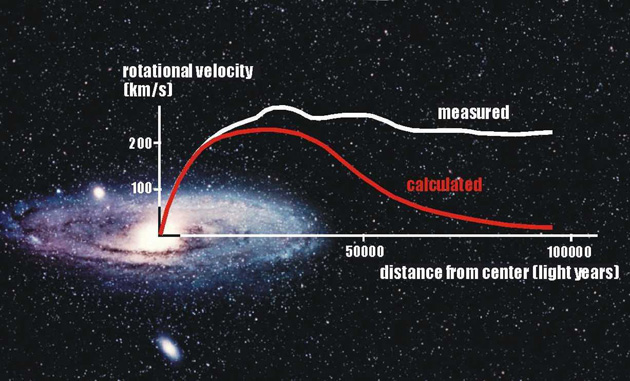
\includegraphics[width=0.6\linewidth,angle=0]{figures/curva_di_rotazione.jpg}
\caption{Confronto tra la curva di rotazione predetta dal modello kepleriano (in rosso) basato sulla sola materia visibile e la curva osservata sperimentalmente (in bianco), caratterizzata da un andamento piatto.}
\label{fig:curva_rotazione}
\end{figure}

Tuttavia, le osservazioni cinematiche mostrano un andamento radicalmente differente: superato il picco iniziale, la curva di rotazione non decade affatto, ma rimane approssimativamente costante a un valore $v_{\mm{max}}$ costante fino a diverse decine di kiloparsec dal centro, come mostrato in Figura \ref{fig:curva_rotazione}.

Per mantenere $v(r) = \text{costante}$ nell'equazione \eqref{eq:andamento_kepleriano}, la massa totale racchiusa non può essere costante, ma deve crescere linearmente con il raggio:
\begin{equation}
M(r) \propto r
\end{equation}
Questo comportamento implica necessariamente la presenza di una considerevole componente di massa non luminosa che domina le regioni esterne della galassia, il cui profilo di densità deve decadere come il quadrato del raggio:
\begin{equation}
\rho(r) \propto \frac{1}{r^2}
\end{equation}
Tale distribuzione di densità è incompatibile con la struttura geometrica a disco tipica della materia barionica visibile in queste galassie. Inoltre, lo studio della cinematica stellare perpendicolare al piano galattico (ovvero le misurazioni effettuate sul moto verticale delle stelle) conferma che questo deficit di massa non è confinato sul piano del disco, ma è distribuito in modo isotropo e sfericamente simmetrico. Si teorizza quindi che ogni galassia a spirale sia immersa in un vasto e massiccio alone di materia oscura a simmetria sferica, che si estende ben oltre i confini della materia visibile.

\subsection{Il Bullet Cluster e gravitational lensing}
\label{subsec:bullet_cluster}

\begin{figure}[htbp]
\centering
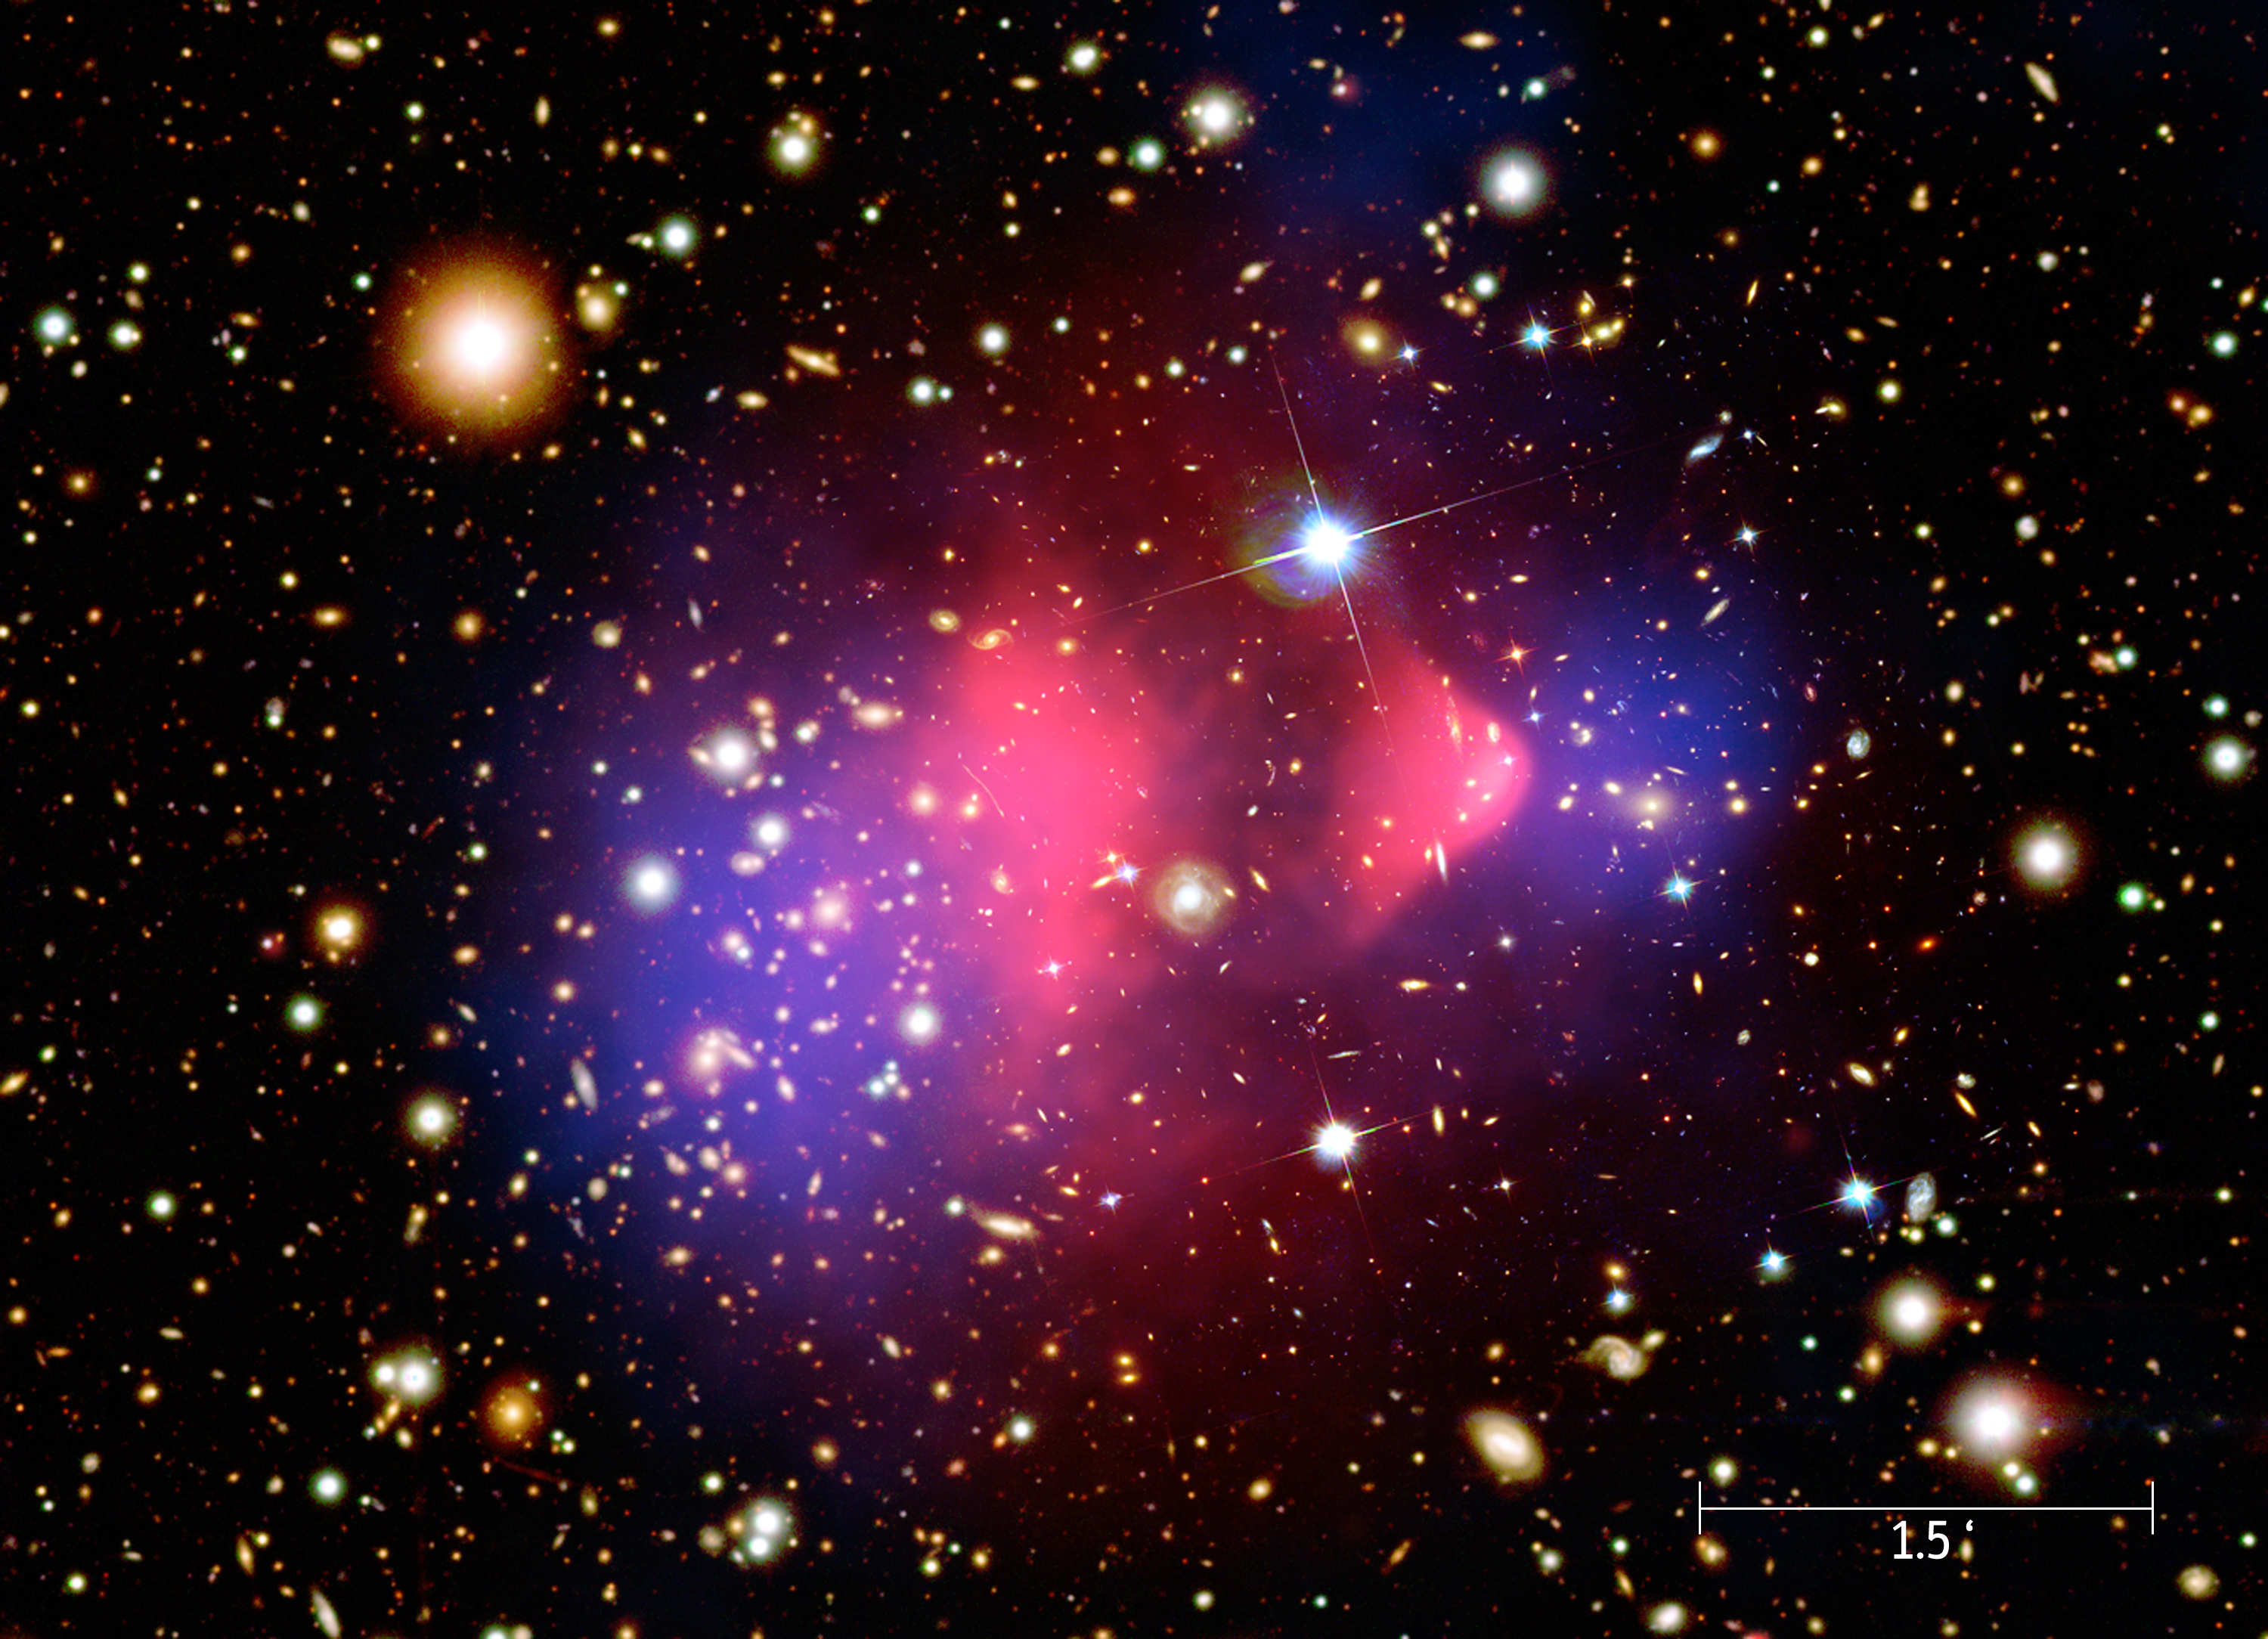
\includegraphics[width=0.6\linewidth,angle=0]{figures/bullet_cluster.jpg}
\caption{Bullet Custer: in rosa il gas intracluster che emette raggi X, in blu la distribuzione di materia oscura calcolata tramite \textit{gravitational lensing}. Sullo sfondo la stessa immagine vista nello spettro ottico. Immagine presa da \cite{chandra_bullet_2006}}
\label{fig:bullet_cluster}
\end{figure}

Un'altra convincente prova dell'esistenza di materia oscura, proviene dallo studio dell'ammasso di galassie \textit{Bullet Cluster} (1E 0657-558). Questo sistema è il risultato di una collisione ad alta velocità tra due sotto-ammassi di galassie.

In un ammasso galattico, la componente barionica dominante in termini di massa non è rappresentata dalle stelle delle galassie, bensì dal gas interstellare caldo, detto \textit{Intracluster medium} (ICM), che permea lo spazio tra una galassia e l'altra. Durante la collisione, la materia barionica ha manifestato comportamenti macroscopicamente distinti:
\begin{itemize}
    \item \textbf{Il gas intra-ammasso}, interagendo attraverso interazione elettromagnetica, ha subito un forte attrito che ne ha causato il rallentamento e il conseguente riscaldamento, lasciandolo confinato nella regione centrale dello scontro, dove si nota una forte emissione di raggi X termici di frenamento (\textit{bremsstrahlung}).
    \item \textbf{Le componenti stellari} delle galassie, essendo sistemi compatti, sono passate oltre la zona di impatto senza subire rallentamenti significativi.
\end{itemize}

Se la dinamica cosmologica fosse governata esclusivamente dalla materia barionica soggetta a leggi gravitazionali modificate (come la teoria MOND, \textit{Modified Newtonian Dynamics}, che cerca di giustificare l'andamento della curva di rotazione delle galassie a spirale senza introdurre la materia oscura), il minimo del potenziale gravitazionale del sistema dovrebbe coincidere con il centro della distribuzione spaziale del gas, dove risiede la quasi totalità della massa ordinaria.

Tuttavia, le mappe della densità di massa totale ottenute mediante tecniche di \textit{gravitational lensing}, sfruttando le distorsioni geometriche della luce proveniente da galassie di fondo, mostrano che i minimi del potenziale gravitazionale si trovano in corrispondenza delle componenti galattiche che non hanno subito collisioni, nettamente separati e spazialmente disaccoppiati dal plasma barionico, come visibile in Figura \ref{fig:bullet_cluster}.

Questo fenomeno di disaccoppiamento spaziale tra la massa visibile e il centro di massa gravitazionale fornisce la prova empirica che la maggior parte della materia nel sistema è costituita da una componente invisibile che sicuramente non interagisce nè tramite interazione elettromagnetica nè forte: la materia oscura.


\subsection{Anisotropie della Radiazione Cosmica di Fondo (CMB)}
\label{subsec:cmb}

Mentre le curve di rotazione galattiche e il Bullet Cluster costituiscono evidenze di natura astrofisica e locale, la Radiazione Cosmica di Fondo (CMB, \textit{Cosmic Microwave Background}) fornisce una prova di natura prettamente cosmologica, legata all'evoluzione dell'Universo primordiale. 

La CMB rappresenta la radiazione fossile emessa all'epoca della ricombinazione (circa $380\,000$ anni dopo il Big Bang), quando la temperatura del cosmo discese sotto la soglia dei $\sim 3000\text{ K}$. A queste energie, i protoni e gli elettroni liberi si legarono per formare idrogeno neutro; questo evento causò il disaccoppiamento dei fotoni dal plasma barionico, rendendo l'Universo trasparente alla radiazione. I fotoni primordiali, in viaggio da allora, hanno subito un drastico redshift a causa dell'espansione cosmologica fino a raggiungere i nostri rivelatori.

La mappa della CMB (Figura \ref{fig:CMB}) mostra uno spettro di corpo nero quasi perfetto a una temperatura media di $T_0 \approx 2.725\text{ K}$, caratterizzato da microscopiche fluttuazioni termiche dell'ordine di $\Delta T / T_0 \sim 10^{-5}$. Dal punto di vista fisico, tali fluttuazioni (chiamate anisotropie della CMB) rappresentano la firma termica delle onde acustiche primordiali: esse costituiscono i "semi" da cui si sono formate le attuali strutture cosmiche, come galassie e ammassi, e offrono una prova decisiva della presenza di materia oscura.

Nel plasma antecedente alla ricombinazione, la materia barionica era soggetta a due forze contrapposte: l'attrazione gravitazionale, che ne favoriva il collasso, e la pressione di radiazione esercitata dai fotoni (fortemente accoppiati agli elettroni tramite \textit{scattering Thomson}), che tendeva a far espandere il fluido verso l'esterno. Questa competizione generava delle vere e proprie oscillazioni acustiche.

In questo scenario, il ruolo della materia oscura risulta fondamentale. Essendo priva di accoppiamento elettromagnetico, la materia oscura non risentiva della pressione di radiazione dei fotoni. Di conseguenza, ha potuto iniziare il proprio collasso gravitazionale molto prima della ricombinazione, scavando pozzi di potenziale gravitazionale profondi e stabili all'interno dei quali la materia barionica è successivamente precipitata.

L'analisi statistica di queste anisotropie viene eseguita scomponendo la mappa in armoniche sferiche per ricavarne lo spettro di potenza angolare (Figura \ref{fig:PowerSpectrum}). L'altezza e la posizione dei picchi acustici di questo spettro forniscono una misura diretta e ad altissima precisione dei parametri cosmologici. 

\begin{figure}[h]
\centering
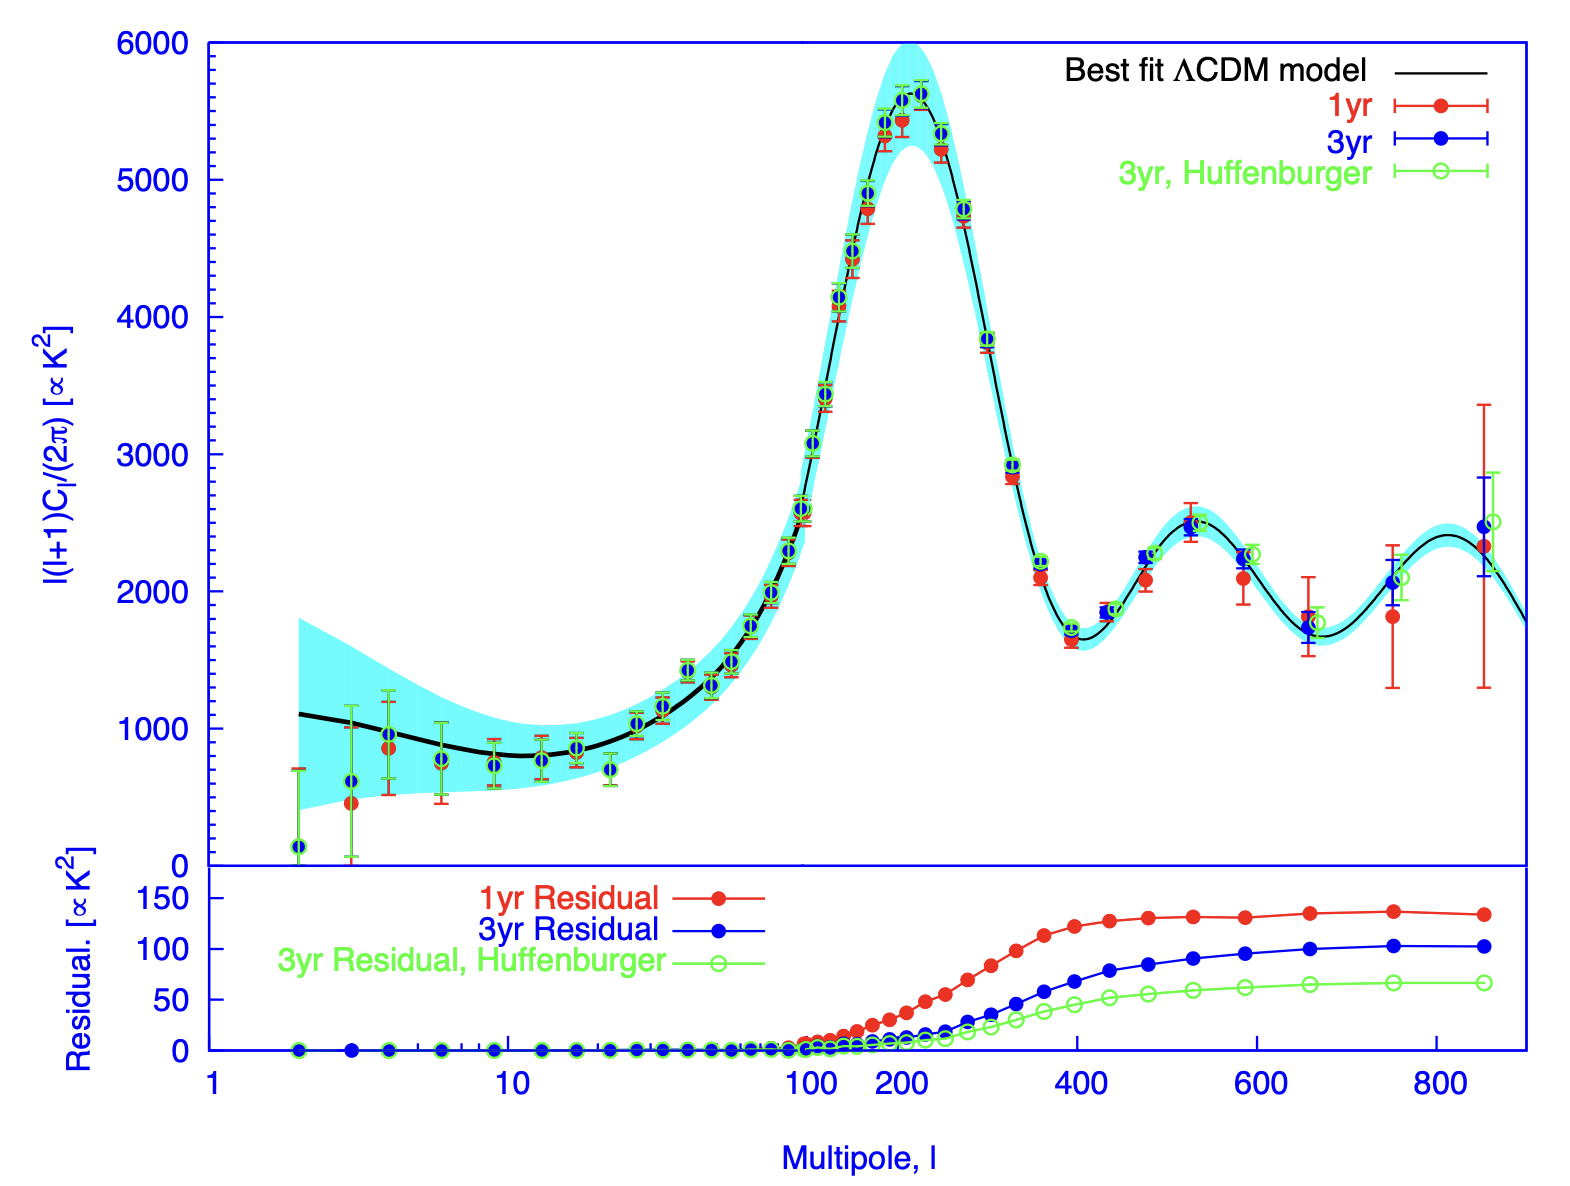
\includegraphics[width=0.6\linewidth]{figures/spettro_pot_ang.png}
\caption{Spettro di potenza angolare ottenuto da WMAP-1 (rosso) e WMAP-3 (blu) confrontato con la previsione teorica del modello $\Lambda$CDM (linea nera). L'asse delle ascisse rappresenta il momento di multipolo $\ell$, mentre l'asse delle ordinate mostra l'ampiezza delle anisotropie della CMB. Immagine tratta da \cite{Souradeep2006AngularPS}.}
\label{fig:PowerSpectrum}
\end{figure}

Il primo picco, situato a una scala angolare $\theta \approx 1^\circ$ (corrispondente al momento di multipolo $\ell \approx 220$), rappresenta l'ampiezza apparente delle regioni di plasma che hanno fatto in tempo a subire esattamente una sola massima compressione prima del disaccoppiamento. La sua posizione fornisce la prova sperimentale che l'Universo è geometricamente piatto ($\Omega = 1$).

L'evidenza più marcata della materia oscura emerge dall'analisi dei picchi successivi. Il secondo picco, corrispondente alla prima fase di massima rarefazione (il "rimbalzo" del plasma verso l'esterno), risulta significativamente più basso rispetto al primo. Questo smorzamento è dovuto proprio all'azione della materia oscura: non subendo la spinta della radiazione, la materia oscura è rimasta confinata nel fondo dei pozzi di potenziale, esercitando una forte attrazione gravitazionale che ha ostacolato e frenato l'espansione del fluido barionico verso l'esterno. Il terzo picco, legato alla seconda compressione massima, beneficia nuovamente del potenziale gravitazionale della materia oscura, mostrando un'ampiezza paragonabile al secondo picco.

I dati sperimentali confermano con straordinaria precisione il modello cosmologico standard $\Lambda\text{CDM}$, stabilendo che la materia oscura fredda (CDM) costituisce circa il $26.8\%$ della densità di energia totale dell'Universo, a fronte di un esiguo $4.9\%$ attribuibile alla materia barionica ordinaria.

\begin{figure}[htbp]
\centering
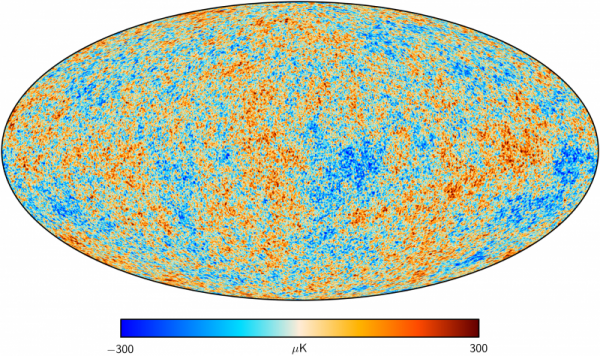
\includegraphics[width=0.6\linewidth]{figures/planck_int_cmb_0.png}
\caption{Mappa delle anisotropie di temperatura della radiazione cosmica di fondo ricostruita con i dati del satellite Planck. La CMB si comporta come un corpo nero con una temperatura media di $2.725\text{ K}$, presentando minime deviazioni da un emettitore perfetto. Tali deviazioni si manifestano come fluttuazioni termiche dell'ordine di circa $\pm 300\ \mu\text{K}$ (con variazioni medie di circa $18\ \mu\text{K}$), le quali riflettono le anisotropie primordiali della densità di materia. Immagine tratta da \cite{Planck2018Overview}.}
\label{fig:CMB}
\end{figure}

\section{Possibili candidati di Materia Oscura}
\label{sec:candidati}

Le evidenze cinematiche e cosmologiche discusse nei paragrafi precedenti delineano l'esistenza di una nuova forma di materia la cui natura fondamentale resta ignota, ma di cui è possibile tracciare un preciso profilo identitario. Affinché un candidato particellare sia accettabile, deve soddisfare simultaneamente quattro requisiti fondamentali:
\begin{enumerate}
    \item \textbf{Massivo:} dati gli effetti gravitazionali sulle galassie a spirale
    \item \textbf{Stabile o quasi-stabile:} con un tempo di vita medio nettamente superiore all'età dell'Universo ($\tau \gg 13.8 \times 10^9 \text{ anni}$), garantendone la permanenza dall'epoca della ricombinazione fino all'Universo locale contemporaneo.
    \item \textbf{Non luminoso:} elettricamente neutro e privo di carica di colore, per giustificare l'assenza di interazioni elettromagnetiche e forti dirette.
    \item \textbf{Non relativistico:} per permettere il corretto collasso gravitazionale delle strutture su piccola scala.
\end{enumerate}

I candidati di natura barionica non luminosa, storicamente raggruppati sotto il nome di MACHOs (\textit{Massive Compact Halo Objects}), sono oggi sperimentalmente esclusi dai dati ottenuti attraverso \textit{microlensing}. Si rende quindi necessario esplorare scenari di materia oscura non barionica.

Per catalogare la vasta gamma di particelle ipotizzate dalla fisica teorica, una prima fondamentale distinzione risiede nella cinematica delle particelle e nel loro impatto sulla formazione delle strutture:
\begin{itemize}
    \item \textbf{Hot Dark Matter (HDM):} Costituita da particelle leggere (scala dell'eV) e relativistiche. Avendo un'energia cinetica così elevata, è molto probabile si siano formati prima i superammassi che poi si sono divisi in strutture più piccole. Il modello che spiega questa evoluzione è detto Top-Down ed è oggi escluso dalle osservazioni della struttura su grande scala dell'Universo.
    \item \textbf{Cold Dark Matter (CDM):} Composta da particelle massive o nate cinematicamente fredde, con velocità non relativistiche ($v \ll c$) già nelle prime fasi evolutive. Il modello evolutivo di tipo Bottom-Up predice invece la formazione iniziale di piccole strutture, poi aggregatesi in ammassi più grandi.
\end{itemize}

\begin{figure}[t]
\centering
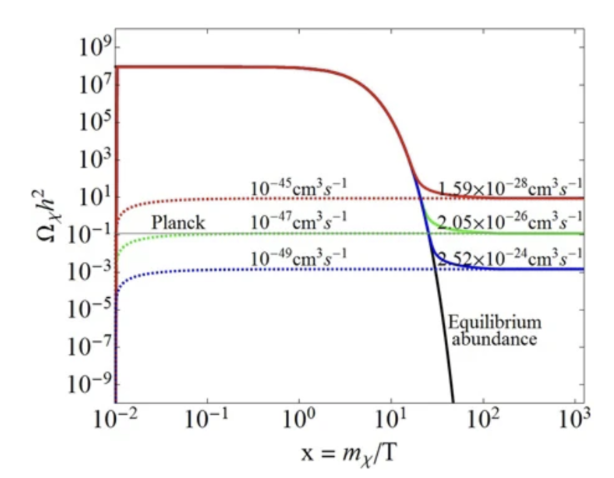
\includegraphics[width=0.6\linewidth,angle=0]{figures/freeze_in_out.png}
\caption{Confronto cinematico tra i meccanismi di produzione termica (\textit{freeze-out}, linee continue a destra) e non termica (\textit{freeze-in}, linee tratteggiate a sinistra) in funzione del parametro evolutivo $x = m_\chi / T$. La linea grigia orizzontale indica il valore della densità relitta misurato dal satellite Planck ($\Omega_{\chi} h^2 \approx 0.12$). Nel \textit{freeze-out}, le curve deviano dall'abbondanza di equilibrio termico a seconda della sezione d'urto di annichilazione. La linea verde, che fitta perfettamente i dati di Planck, corrisponde al valore ideale dell'interazione debole ($\sim 10^{-26} \text{ cm}^3\text{s}^{-1}$, il \textit{WIMP miracle}). Nel \textit{freeze-in}, l'abbondanza parte da zero e cresce per rari urti termici fino a stabilizzarsi; la linea verde tratteggiata rappresenta il valore di sezione d'urto di produzione necessario a riprodurre correttamente la densità di materia oscura attuale ($\sim 10^{-47} \text{ cm}^3\text{s}^{-1}$, impossibile da rilevare in esperimenti come CRESST). Immagine tratta da \cite{Chu2012DM}.}
\label{fig:freeze_in_out}
\end{figure}

Un secondo criterio di classificazione, riguarda il meccanismo di produzione della densità di materia oscura ($\Omega_{\mm{DM}}$) misurata oggi, illustrato in Figura \ref{fig:freeze_in_out}:
\begin{itemize}
    \item \textbf{Produzione Termica:} La materia oscura si trovava inizialmente in equilibrio termico e chimico con il plasma del Modello Standard nell'Universo primordiale, attraverso interazioni della forma
    \begin{equation}
        \text{DM$\,$+$\,$DM$\,$(+$\,$DM...)}\leftrightarrow \text{SM particles}.
    \end{equation} 
    La sua abbondanza attuale viene determinata dal meccanismo di \textit{freeze-out}, ovvero lo spegnimento delle reazioni di annichilazione dovuto all'espansione del cosmo.
    
    \item \textbf{Produzione Non Termica:} La materia oscura non termica non raggiunge l'equilibrio con le particelle del Modello Standard nel plasma primordiale, poiché governata da un'interazione estremamente più debole di quella nucleare debole. Viene generata per via quantistica o geometrica (come nei meccanismi di \textit{freeze-in} o di disallineamento), nascendo cinematicamente fredda anche se caratterizzata da una massa estremamente esigua.
\end{itemize}

I candidati più quotati al giorno d'oggi sono le WIMPs e gli assioni, entrambi appartenenti alla famiglia della Cold Dark Matter. Uno schema di tutti i possibili candidati in funzione della massa è riportato in Figura \ref{fig:candidati}

\begin{figure}[htbp]
\centering
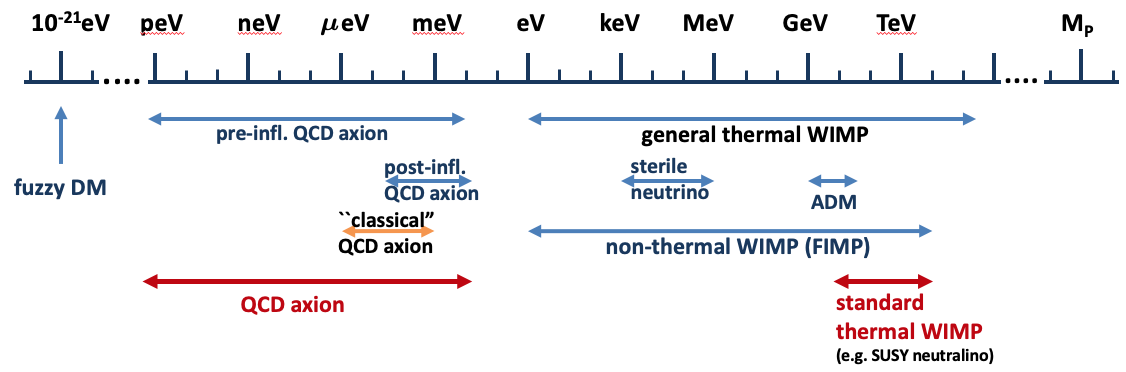
\includegraphics[width=1\linewidth,angle=0]{figures/dmmassrange_appecdmddreport_2020_v102.png}
\caption{Principali candidati di materia oscura divisi in range di massa, dal peV (assioni) alla massa di Planck ($1.2\cdot10^{19} \, \text{GeV}$)}
\label{fig:candidati}
\end{figure}

\subsection{WIMPs (Weakly Interacting Massive Particles)}
\label{subsec:wimps}

Le WIMPs rappresentano la classe di candidati di tipo CDM termico più accreditata e costituiscono l'obiettivo primario di esperimenti di rivelazione diretta come CRESST. Si tratta di particelle ipotetiche stabili, con una massa tipicamente compresa tra i $\mathrm{GeV}$ e i $\mathrm{TeV}$, che interagiscono con la materia ordinaria esclusivamente tramite la gravità e l'interazione nucleare debole (o un'interazione con sezione d'urto analoga).

Essendo candidati a produzione termica, nelle prime fasi dell'Universo queste particelle si trovavano in equilibrio chimico e termico con il plasma primordiale attraverso processi di creazione e annichilazione del tipo $\chi \bar{\chi} \rightleftharpoons \text{SM} \, \text{SM}$, in cui i due tassi di reazione si compensavano.

A seguito dell'espansione dell'Universo, la temperatura del plasma è scesa, e quando $ T < m_\chi$, il processo di creazione si è spento, mentre il processo di annichilazione, seppur rallentato dalla progressiva diluizione delle WIMP, è proseguito.

Quando il tasso di espansione dell'Universo ($H$) è diventato confrontabile e poi superiore al tasso di annichilazione, le particelle non sono più riuscite a incontrarsi efficacemente. Il processo di annichilazione si è congelato (\textit{freeze-out}) e l'abbondanza per unità di volume comovente ha determinato la densità relitta osservata oggi.

È interessante notare come le conclusioni teoriche ricavate inserendo i valori tipici della sezione d'urto dell'interazione debole conducano a una densità relitta che coincide sorprendentemente con i dati sperimentali osservati dal satellite Planck. Questa convergenza spontanea prende il nome di \textit{WIMP miracle}, e fornisce una solida giustificazione teorica alla ricerca di tali candidati nella finestra energetica dei $\mathrm{GeV}$-$\mathrm{TeV}$.

\subsection{Assioni}
\label{subsec:assioni}

L'assione è un candidato di materia oscura fredda a produzione non termica. La sua esistenza non è stata ipotizzata inizialmente per spiegare la massa mancante dell'Universo, ma per risolvere un problema teorico della fisica delle particelle noto come \textit{problema della CP forte}. Le equazioni della Cromodinamica Quantistica (QCD) permettono teoricamente una violazione della simmetria di Carica e Parità (CP) per le interazioni forti, che però non è mai stata osservata. 
Per giustificare ciò è stata ipotizzata una nuova simmetria globale, la cui rottura spontanea genera l'assione. Tramite questo meccanismo, il parametro che regola la violazione di CP viene guidato dinamicamente a zero.

La caratteristica principale dell'assione è la sua massa estremamente ridotta, che i modelli cosmologici attestano nella finestra dei micro-elettronvolt ($m_a \sim 10^{-6} - 10^{-3} \text{ eV}$).

Essendo particelle così leggere, si potrebbe erroneamente dedurre che gli assioni si muovano a velocità relativistiche, comportandosi come materia oscura calda. Tuttavia, queste particelle state generate da un processo detto meccanismo di disallineamento, che prevede la creazione di queste particelle a partire da oscillazioni del campo quantistico dell'assione, poiché esso si trovava disallineato rispetto al suo stato di minima energia. Queste oscillazioni si comportano come particelle con momento lineare quasi nullo, e dunque un candidato di CDM.

Dal punto di vista sperimentale, l'assione interagisce in modo talmente debole da non poter essere rivelato tramite gli urti nucleari cercati da esperimenti come CRESST. La ricerca di queste particelle avviene quindi tramite esperimenti radicalmente diversi dalla ricerca WIMP, basati sull'uso di speciali cavità risonanti note come aloscopi, che sfruttano la caratteristica degli assioni di convertirsi in fotoni (tipicamente nella frequenza delle microonde) quando attraversano un campo magnetico molto intenso.

\section{Tecniche di rivelazione}
\label{sec:rivelazione}

Rivelare la materia oscura rappresenta una delle sfide più complesse della fisica contemporanea, poiché l'unica interazione sperimentalmente accertata su scala macroscopica è quella di natura gravitazionale. Tuttavia, assumendo l'ipotesi che la materia oscura sia composta da WIMPs, si aprono tre possibili canali di indagine, basati sul potenziale accoppiamento con le particelle del Modello Standard.

\begin{itemize}
    \item \textbf{produzione nei collider}, in cui si tenta di produrre particelle di materia oscura facendo collidere particelle note ad altissime energie, cercandone la traccia sotto forma di energia o momento mancante nei prodotti di reazione.
    \item \textbf{rivelazione indiretta}, effettuata principalmente tramite telescopi terrestri e spaziali; questa tecnica mira a individuare i prodotti stabili derivanti dall'annichilazione o dal decadimento di particelle di materia oscura in zone ad alta densità cosmica (come il centro galattico), sotto forma di eccessi di raggi gamma, neutrini o antimateria.
    \item \textbf{rivelazione diretta}, consiste nell'esaminare in laboratori sotterranei gli urti elastici delle particelle di materia oscura del nostro alone galattico contro i nuclei atomici di un bersaglio (nel caso di CRESST, cristalli di $\text{CaWO}_4$).
\end{itemize}


I tre metodi di indagine sono riassunti schematicamente in Figura \ref{fig:schema_DM} e verranno analizzati singolarmente nei successivi paragrafi.

\begin{figure}[htbp]
\centering
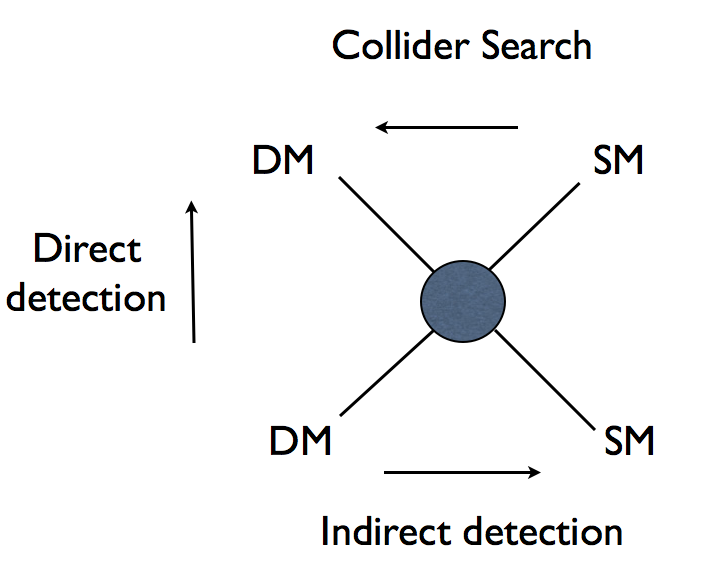
\includegraphics[width=0.5\linewidth,angle=0]{figures/scheme.png}
\caption{Rappresentazione schematica delle principali strategie di rivelazione della materia oscura.}
\label{fig:schema_DM}
\end{figure}

\subsection{Produzione nei collider}
La ricerca di materia oscura mediante collider viene svolta principalmente al \textit{Large Hadron Collider} (LHC), facendo scontrare particelle del Modello Standard ad alta energia e andando a cercare un deficit nel bilancio dell'energia o del momento totale delle particelle create. 

Tuttavia, trovare una nuova particella con questa tecnica non assicurerebbe automaticamente di aver individuato la materia oscura, ma si renderebbe necessaria una conferma indipendente tramite la rivelazione diretta o indiretta. Inoltre, date le brevi scale temporali e le distanze percorse dalle particelle all'interno dell'apparato sperimentale, non si avrebbe la certezza che la particella prodotta abbia una vita media paragonabile all'età dell'Universo, caratteristica invece fondamentale per la materia oscura.

\subsection{Rivelazione indiretta}
\label{subsec:indiretta}

Sebbene nel paragrafo \ref{subsec:wimps} si sia descritto il meccanismo di \textit{freeze-out} come il congelamento delle annichilazioni dovuto alla drastica diminuzione della densità di materia oscura nell'Universo, questo scenario assume un cosmo  omogeneo e non si applica su scala locale. All'interno delle strutture legate gravitazionalmente, come le galassie o gli ammassi di galassie, la materia oscura si è accumulata formando aloni ad altissima densità. In queste regioni, il tasso di interazione è sufficientemente elevato da consentire ai processi di annichilazione di proseguire attivamente anche nell'Universo contemporaneo.

La rivelazione indiretta si propone quindi di individuare i prodotti stabili derivanti da queste annichilazioni. Il processo genera particelle del Modello Standard che, attraverso successivi decadimenti, si convertono in flussi di raggi gamma, neutrini ad alta energia e antimateria cosmica (come antiprotoni e positroni). Questi segnali vengono successivamente catturati da telescopi e apparati sperimentali terrestri, come l'osservatorio per raggi gamma \textit{MAGIC} o il rivelatore di neutrini \textit{IceCube} al Polo Sud, oppure da spettrometri spaziali orbitanti a bordo della Stazione Spaziale Internazionale, come l'esperimento \textit{AMS-02}.

\subsection{Rivelazione diretta}
\label{subsec:rivelazione_diretta}

La rivelazione diretta tenta di catturare i rarissimi eventi in cui una WIMP appartenente all'alone di materia oscura attraversa un rivelatore posto in un laboratorio sotterraneo e subisce uno scattering elastico coerente contro il nucleo atomico di un materiale bersaglio.

\begin{figure} [b]
    \centering
    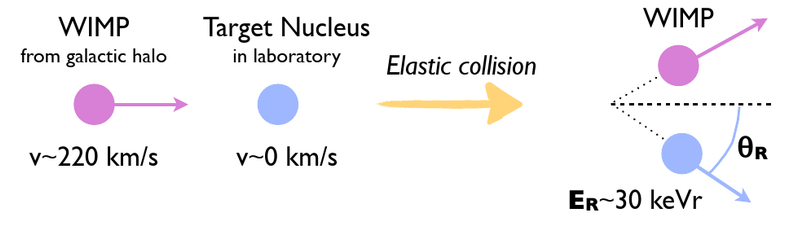
\includegraphics[width=0.6\linewidth]{figures/A-schematic-of-dark-matter-WIMP-elastic-scattering-off-a-target-nucleus.ppm.png}
    \caption{Scattering tra WIMP e nucleo target nel SR del laboratorio. In questo caso il massimo trasferimento di energia si avrebbe per $\theta_R = 0$}
    \label{fig:scattering}
\end{figure}

Il processo può essere modellizzato cinematicamente come un urto elastico a due corpi non relativistico (Figura \ref{fig:scattering}) tra una particella di materia oscura $\chi$ di massa $m_\chi$ e un nucleo a riposo di massa $m_N$. Nell'approssimazione in cui la WIMP possiede una velocità iniziale $v$ tipica del profilo galattico ($v \approx 220\,\mm{km/s}$), l'energia di rinculo $E_R$ trasferita al nucleo a seguito dell'impatto dipende dall'angolo di scattering $\theta$ nel sistema del centro di massa ed è espressa dalla relazione:

\begin{equation}
E_R = \frac{\mu_N^2 v^2}{m_N} (1 - \cos\theta)
\label{eq:energia_rinculo}
\end{equation}

dove $\mu_N$ rappresenta la massa ridotta del sistema WIMP-nucleo, definita come:

\begin{equation}
\mu_N = \frac{m_\chi m_N}{m_\chi + m_N}
\label{eq:massa_ridotta}
\end{equation}

Dall'equazione \ref{eq:energia_rinculo} si deduce che l'energia massima trasferita ($E_{\mm{max}}$) si ottiene nel caso $\theta = \pi$:

\begin{equation}
E_{\mm{max}} = \frac{2 \mu_N^2 v^2}{m_N}
\label{eq:energia_massima}
\end{equation}

Considerando i valori tipici previsti per le WIMP ($m_\chi \sim 100\,\mm{GeV}$) e le masse dei nuclei comunemente impiegati nei rivelatori (come l'Ossigeno, il Calcio o il Tungsteno nel caso dei cristalli di $\mm{CaWO}_4$ di CRESST), l'energia di rinculo risulta confinata in un range molto basso, tipicamente compresa tra frazioni di $\mm{keV}$ e poche decine di $\mm{keV}$. La difficoltà della rivelazione diretta consiste proprio nello sviluppare esperimenti che abbiano una sensibilità tale da poter misurare rilasci di energia così esigui.

\begin{figure}[htbp]
    \centering
    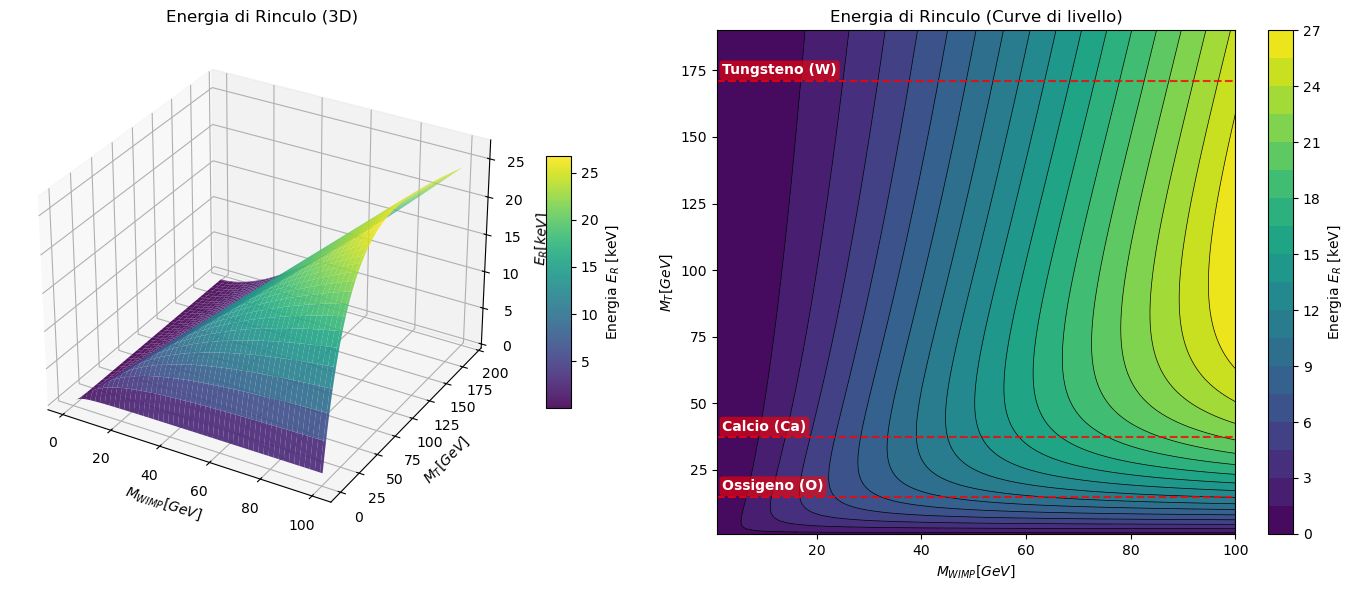
\includegraphics[width=1\linewidth]{figures/Energia_rinculo.png}
    \caption{Energia di rinculo (\ref{eq:energia_massima}) in funzione della massa della WIMP ($M_{WIMP}$) e della massa del nucleo bersaglio ($M_T$). A sinistra è mostrato l'andamento tridimensionale della funzione, mentre a destra è riportato il grafico a curve di livello, dove le linee tratteggiate rosse indicano le masse dei target di Ossigeno, Calcio e Tungsteno. Si nota come il trasferimento di energia sia massimo nel caso $M_{WIMP} \approx M_T$. Per questo motivo l'esperimento CRESST utilizza 3 bersagli con massa diversa, in modo da massimizzare la sensibilità su un ampio spettro di masse della materia oscura.}
    \label{fig:Energia_rinculo}
\end{figure}

\subsubsection{Tasso di eventi e sezione d'urto}
\label{subsec:rate_sezionedurto}
Il tasso di eventi stima quanti urti ci si aspetta di osservare in un intervallo di tempo e si esprime in numero di interazioni per unità di tempo e massa del rivelatore. La formula semplificata, che suppone la velocità delle particelle di materia oscura nell'alone $v$ costante è data da:

\begin{equation}
R = \frac{\rho_0}{m_\chi} \frac{\sigma_0}{m_N} v
\label{eq:rate_semplice}
\end{equation}
dove $\rho_0$ è la densità locale di materia oscura (stimata a circa $0.3\,\mm{GeV/cm}^3$), $m_\chi$ è la massa della WIMP, $m_N$ è la massa del nucleo bersaglio del rivelatore e $\sigma_0$ la sezione d'urto di scattering tra la WIMP e il nucleo

Nella realtà sperimentale, le particelle di materia oscura non viaggiano tutte alla stessa velocità, ma seguono una distribuzione statistica all'interno dell'alone galattico. Per questa ragione, l'espressione completa del tasso differenziale di eventi è data da:

\begin{equation}
\frac{\dd R}{\dd E_R} = \frac{\rho_0}{m_\chi m_N} \int_{v_{\mm{min}}}^{v_{\mm{fuga}}} v \cdot f(\vec{v}) \frac{\dd\sigma}{\dd E_R} \, \dd^3 v
\label{eq:rate_differenziale}
\end{equation}
dove $f(\vec{v})$ è la funzione di distribuzione delle velocità delle WIMP nel sistema di riferimento della Terra, $\frac{\dd\sigma}{\dd E_R}$ è la sezione d'urto differenziale di scattering, mentre $v_{\mm{min}}$ e $v_{\mm{esc}}$ sono rispettivamente la minima velocità che una WIMP deve possedere per trasferire un'energia $E_R$, e la velocità di fuga dalla nostra galassia.

La sezione d'urto differenziale $\frac{\dd\sigma}{\dd E_R}$ si articola in due contributi: uno dipendente dallo spin del nucleo atomico (\textit{spin-dependent}) e uno indipendente da esso (\textit{spin-independent}). Concentrando l'analisi esclusivamente sul canale indipendente dallo spin, la sezione d'urto differenziale risulta proporzionale al quadrato del numero di massa del nucleo bersaglio ($A^2$) e al fattore di forma nucleare $F^2(E_R)$:

\begin{equation}
\frac{\dd\sigma_{\mm{SI}}}{\dd E_R} \propto A^2 \cdot F^2(E_R)
\end{equation}

Il fattore di forma riflette la natura estesa del nucleo atomico. Per energie di rinculo che tendono a zero ($E_R \to 0$), il fattore di forma $F^2(E_R) \to 1$ e la probabilità di interazione è massima. Al contrario, all'aumentare dell'energia trasferita, il valore di $F^2(E_R)$ decresce rapidamente.

Data la proporzionalità tra la sezione d'urto differenziale e il quadrato del numero atomico $A^2$, si potrebbe ipotizzare di utilizzare esclusivamente elementi molto pesanti. Tuttavia, come evidenziato in \ref{eq:energia_massima} e in Figura \ref{fig:Energia_rinculo}, qualora la massa della WIMP fosse di qualche $\mm{GeV}$, l'energia trasferita sarebbe così bassa da non poter essere rivelata dagli strumenti. Per questa ragione CRESST utilizza cristalli multielemento: tre elementi diversi per massimizzare l'energia trasferita e la sezione d'urto.

\subsubsection{Tecnologie di rivelazione}
\label{subsubsec:canali_segnali}

Quando una particella di materia oscura urta un nucleo del materiale bersaglio, l'energia di rinculo rilasciata si dissipa nel mezzo attraverso tre canali di segnale fondamentali:

\begin{itemize}
    \item \textbf{Ionizzazione (Carica):} Questo segnale si genera quando l'energia depositata è sufficiente a eccitare o espellere gli elettroni dagli atomi del mezzo. Nei rivelatori a gas nobile liquido (come Xenon o Argon) gli elettroni liberi vengono accelerati da un campo elettrico per produrre un segnale amplificato. Nei rivelatori a semiconduttore, invece, la ionizzazione crea coppie elettrone-lacuna.
    \item \textbf{Scintillazione (Luce):} Molti materiali eccitati dall'urto rilasciano parte dell'energia riemettendo fotoni. I rivelatori che sfruttano questo principio sono detti scintillatori e possono essere costituiti sia da gas nobili liquefatti che da cristalli scintillatori solidi. La luce di scintilazione viene raccolta dai tubi fotomoltiplicatori.
    \item \textbf{Fononi (Calore):} La frazione maggiore dell'energia di rinculo si traduce in vibrazioni del reticolo cristallino del materiale bersaglio, quantizzate sotto forma di fononi. Questa tecnica richiede di operare a temperature criogeniche (prossime allo zero assoluto) per minimizzare il rumore termico spontaneo del cristallo, permettendo di raggiungere soglie energetiche bassissime e risoluzioni estremamente elevate.
\end{itemize}

Gli esperimenti di rivelazione diretta moderni combinano spesso due di questi canali contemporaneamente. Questa strategia è di fondamentale importanza poiché il rapporto tra i due segnali (ad esempio luce e calore) permette di discriminare con altissima efficienza i rinculi nucleari indotti dalle WIMP dai rinculi elettronici dovuti alla radioattività ambientale di fondo, come si vedrà nella Sezione \ref{sec:light_yield}. I diversi approcci tecnologici e i relativi esperimenti di riferimento sono riassunti schematicamente in Figura \ref{fig:approcci}.

\begin{figure}[htbp]
    \centering
    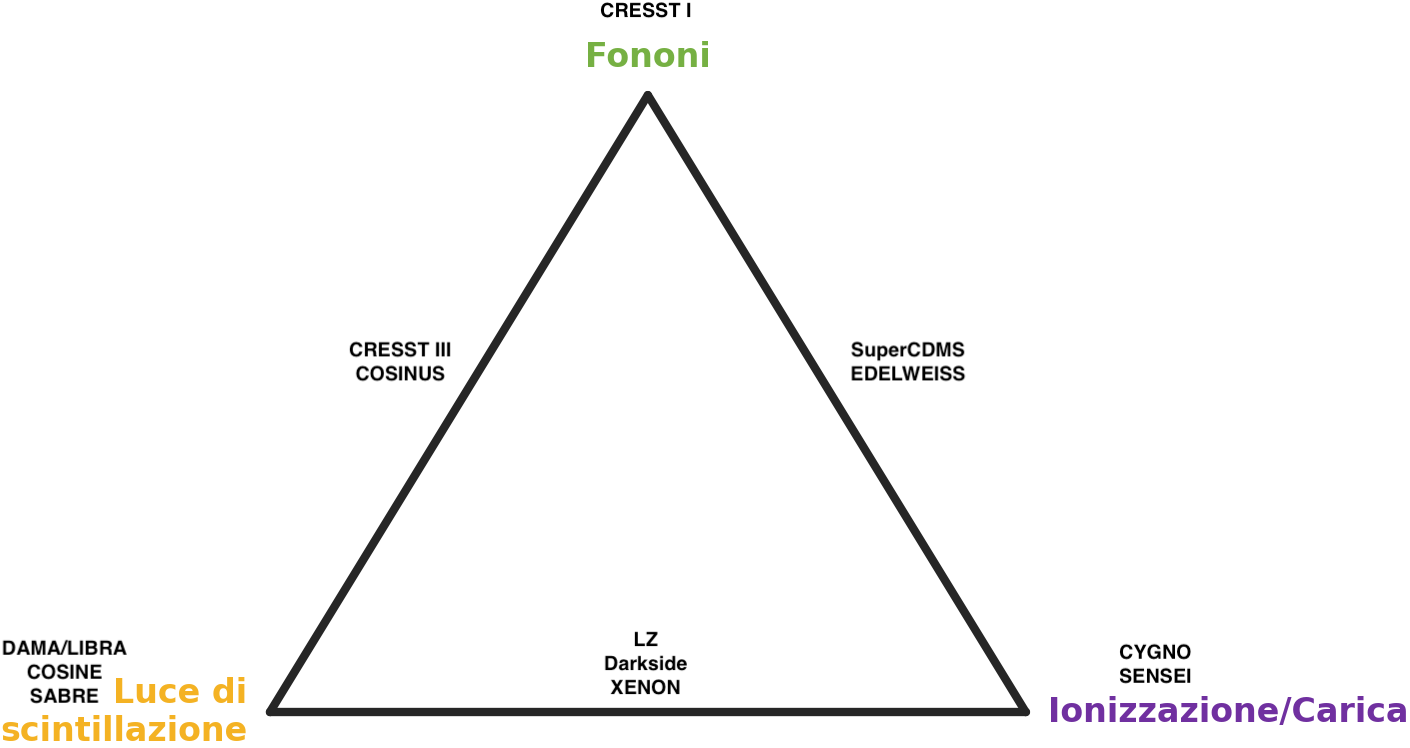
\includegraphics[width=0.8\linewidth]{figures/metodi_DM.png}
    \caption{Rappresentazione schematica dei tre canali di segnale utilizzati nella rivelazione diretta della materia oscura. Gli esperimenti posizionati nelle intersezioni sfruttano la lettura simultanea di due canali per discriminare il fondo radioattivo.}
    \label{fig:approcci}
\end{figure}

\section{Stato dell'arte ed evoluzione delle sensibilità}

In Figura \ref{fig:stato_attuale} è riportato lo stato attuale della ricerca diretta di materia oscura. La regione verde in alto individua lo spazio dei parametri già escluso dai risultati ottenuti. Dal grafico si nota come l'esperimento XENON1T definisca il limite inferiore di sensibilità per WIMP di massa elevata, mentre l'esperimento CRESST III domini la regione delle WIMP a bassa massa grazie all'elevata sensibilità dei rivelatori.

\begin{figure}[htbp]
    \centering
    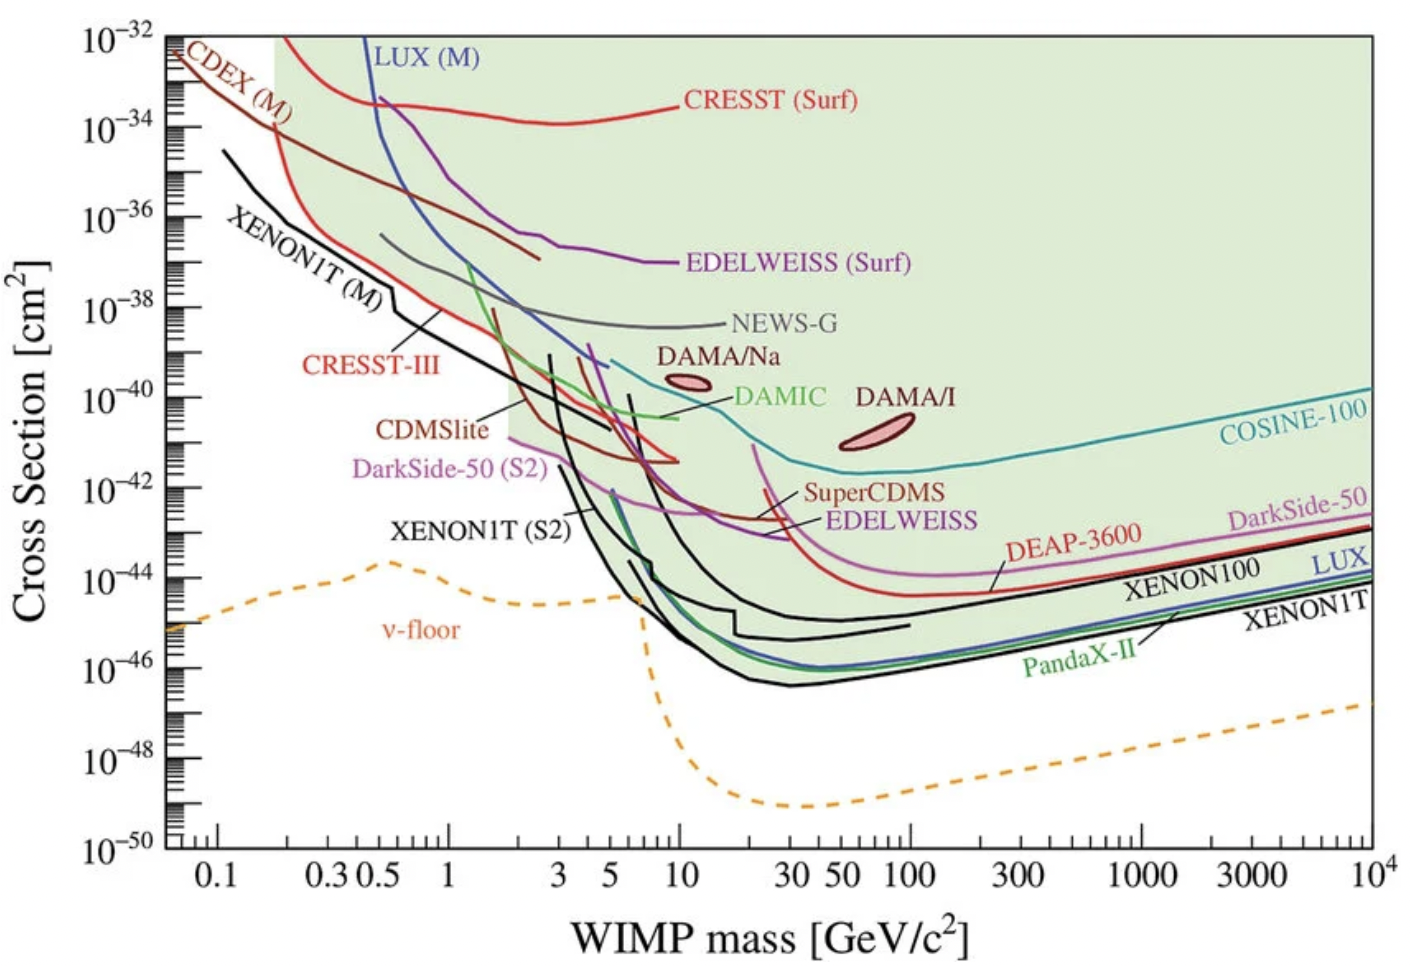
\includegraphics[width=0.8\linewidth]{figures/curva_esclusione_attuale.png}
    \caption{Limiti di esclusione per la sezione d'urto spin-independent WIMP-nucleone. La regione verde rappresenta lo spazio dei parametri escluso dagli esperimenti. Le regioni cerchiate in rosso rappresentano parametri accessibili ottenuti tramite gli esperimenti DAMA/LIBRA, che però non trovano riscontro in esperimenti attuali. Immagine tratta da \cite{Billard2022DirectDM}.}
    \label{fig:stato_attuale}
\end{figure}

Le proiezioni future sono illustrate in Figura \ref{fig:stato_futuro}. È utile notare come la regione verde sia la medesima del grafico precedente, mentre cambiano i valori di sezione d'urto sull'asse verticale. I rivelatori di nuova generazione attualmente in presa dati o in fase di sviluppo in scala di multi-tonnellata (quali XENONnT, LZ e DarkSide-20k) estenderanno ulteriormente la sensibilità, fino a raggiungere il limite intrinseco costituito dalla cosiddetto \textit{neutrino floor}. Parallelamente, per masse inferiori, futuri upgrade di CRESST e altri esperimenti mirati consentiranno di ridurre significativamente lo spazio dei parametri ancora non esplorato.

\begin{figure}[htbp]
    \centering
    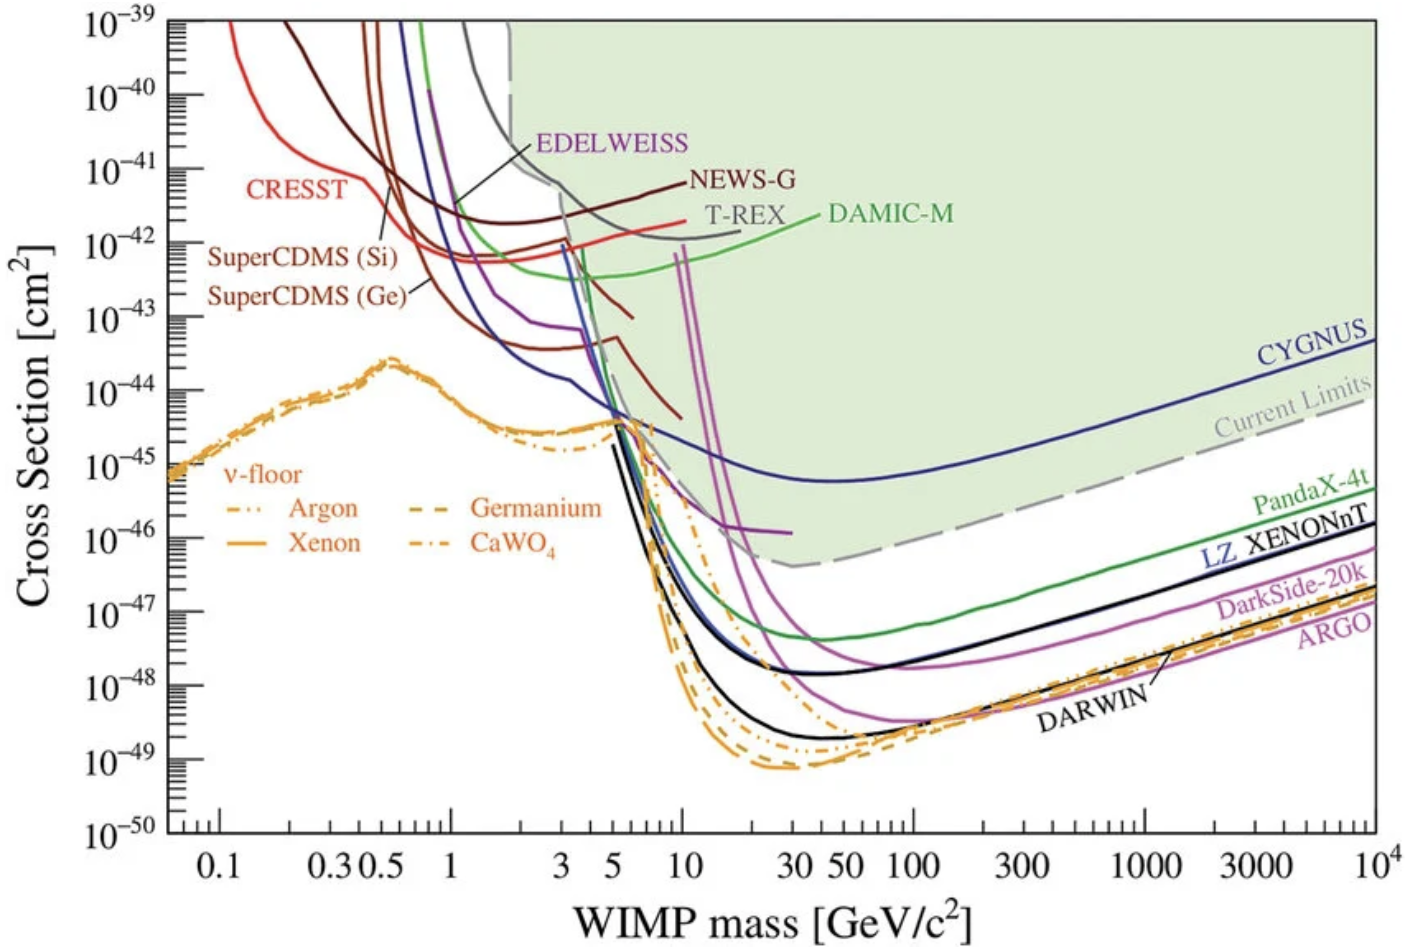
\includegraphics[width=0.8\linewidth]{figures/curva_esclusione_futuro.png}
    \caption{Proiezioni di sensibilità per gli esperimenti di futura generazione. La linea gialla delimita la regione del \textit{neutrino floor}, oltre la quale lo scattering coerente del neutrino costituisce un fondo irriducibile. Le curve inferiori al \textit{Current Limits}, indicano la sensibilità attesa dai futuri esperimenti. Immagine tratta da \cite{Billard2022DirectDM}.}
    \label{fig:stato_futuro}
\end{figure}


 %1
\clearpage{\thispagestyle{empty}\cleardoublepage}
\chapter{L'esperimento CRESST}
\label{ch:CRESST}

L'esperimento CRESST (Cryogenic Rare Event Search with Superconducting Thermometers) è una collaborazione internazionale finalizzata alla ricerca diretta di WIMPs nella regione delle basse masse ($ \leq 1 \text{ GeV}$). L'apparato sperimentale è situato presso i Laboratori Nazionali del Gran Sasso (LNGS) dell'INFN in Italia.
La collocazione sotto 1400 metri di roccia permette di schermare efficacemente il flusso di muoni cosmici.

Per identificare i rari e infinitesimi depositi di energia rilasciati dall'interazione delle WIMP con i nuclei del bersaglio, CRESST impiega rivelatori criogenici a stato solido portati a temperature dell'ordine dei millikelvin (10 mK), prossime allo zero assoluto. Tramite questo processo, che permette di ridurre al minimo il rumore termico di fondo, diventa possibile misurare i minuscoli innalzamenti di temperatura causati dai rinculi nucleari e spingere la soglia di rivelazione energetica a livelli tra i più bassi al mondo, aprendo una finestra osservativa cruciale sulla materia oscura di massa leggera.

\section{Il principio di rivelazione: il doppio canale}
\label{sec:doppio_canale}

Il cuore tecnologico dell'esperimento CRESST risiede nell'utilizzo di target cristallini scintillanti operati come calorimetri criogenici a bassissima temperatura. La scelta del materiale riflette la necessità di massimizzare la sezione d'urto di interazione con le WIMP (\ref{subsec:rate_sezionedurto}) e, al contempo, di disporre di un eccellente mezzo di scintillazione; per queste ragioni, i moduli rivelatori standard di CRESST-III impiegano cristalli di tungstato di calcio ($\text{CaWO}_4$). 

Quando una particella (sia essa una WIMP del segnale o una particella del fondo ambientale) attraversa il cristallo bersaglio, interagisce con la materia depositando una determinata energia $E_{\text{dep}}$. Questo rilascio di energia si propaga nel mezzo dando origine a due processi fisici distinti, che costituiscono i due canali di lettura indipendenti dell'esperimento:

\begin{enumerate}
    \item \textbf{Il canale fononico (calore):} La quasi totalità dell'energia depositata ($>99\%$) viene convertita in vibrazioni reticolari del cristallo, ovvero in fononi non termici. Questi fononi si propagano nel materiale fino a raggiungere la superficie del cristallo, dove un sensore termico ne misura l'innalzamento di temperatura complessivo. Poiché la frazione di energia convertita in calore è pressoché indipendente dal tipo di particella interagente, il canale fononico fornisce una misura precisa e diretta dell'energia depositata, secondo la relazione:
    \begin{equation}
        \Delta T = \frac{E_{\text{dep}}}{C}
    \end{equation}
    dove $C$ è la capacità termica del cristallo bersaglio. A parità di energia depositata, disporre di una capacità termica estremamente bassa permette di massimizzare l'ampiezza del segnale termico $\Delta T$. Per questa ragione i cristalli sono mantenuti a temperature criogeniche dell'ordine del millikelvin, regime in cui la capacità termica segue la legge di Debye ($C \propto T^3$) e risulta drasticamente ridotta rispetto ai valori a temperatura ambiente.
    
    \item \textbf{Il canale fotonico (luce):} Una piccola frazione dell'energia depositata (tipicamente l'1\% o meno) viene emessa sotto forma di fotoni di scintillazione. Per raccogliere questa luce, ogni cristallo di $\text{CaWO}_4$ è accoppiato a un rivelatore di luce indipendente posto nelle immediate vicinanze. La quantità di luce prodotta è fortemente dipendente dalla densità di ionizzazione della particella incidente e, di conseguenza, dalla sua natura (rinculo elettronico dovuto a particelle $\beta/\gamma$ oppure rinculo nucleare dovuto a neutroni, WIMP o particelle $\alpha$).
\end{enumerate}

L'adozione di questa tecnica a doppio canale è l'elemento chiave che conferisce a CRESST la sua straordinaria sensibilità nella ricerca di eventi rari. Mentre il canale fononico determina con precisione l'energia dell'evento e definisce la soglia minima di rivelazione dell'esperimento, il canale fotonico fornisce l'informazione cruciale per identificare la natura dell'interazione. La correlazione tra l'energia misurata sotto forma di calore e quella raccolta sotto forma di luce permette infatti di definire una variabile discriminante fondamentale, il \textit{Light Yield}, di cui si discuterà nel dettaglio nella Sezione~\ref{sec:light_yield}.

\section{Come viene letto il segnale: TES e SQUID}
\label{sec:tes_squid}

La straordinaria sensibilità energetica dell'esperimento CRESST, capace di registrare innalzamenti di temperatura microscopici nei cristalli di $\text{CaWO}_4$, richiede una tecnologia di lettura all'avanguardia. Il sistema di sensoristica si basa sulla combinazione di due dispositivi a superconduzione operanti in sinergia: il \textit{Transition Edge Sensor} (TES), che funge da termometro ad altissima risoluzione, e il \textit{Superconducting Quantum Interference Device} (SQUID), utilizzato come amplificatore di corrente a bassissimo rumore.

\subsubsection{Il Transition Edge Sensor (TES)}

Il TES è un termometro criogenico costituito da una sottile striscia di materiale superconduttore (tipicamente tungsteno) depositato direttamente sulla superficie del cristallo bersaglio e del rivelatore di luce. Il principio di funzionamento sfrutta l'estrema dipendenza della resistenza elettrica dalla temperatura nella stretta regione di transizione tra lo stato normale e lo stato superconduttore.

Mantenendo il sistema a una temperatura di lavoro $T_0$ stabilizzata esattamente al centro di questa curva di transizione, il TES presenta una resistenza parziale. Quando un fonone generato nel cristallo lo colpisce, cede la sua energia causando un microscopico incremento di temperatura $\Delta T$. Poiché la curva della resistenza del TES è estremamente ripida in questa regione, anche un aumento di temperatura dell'ordine di pochi millikelvin provoca un cambiamento significativo della resistenza $\Delta R$ del sensore, come illustrato in Figura \ref{fig:tes_curve}.
\begin{figure}
    \centering
    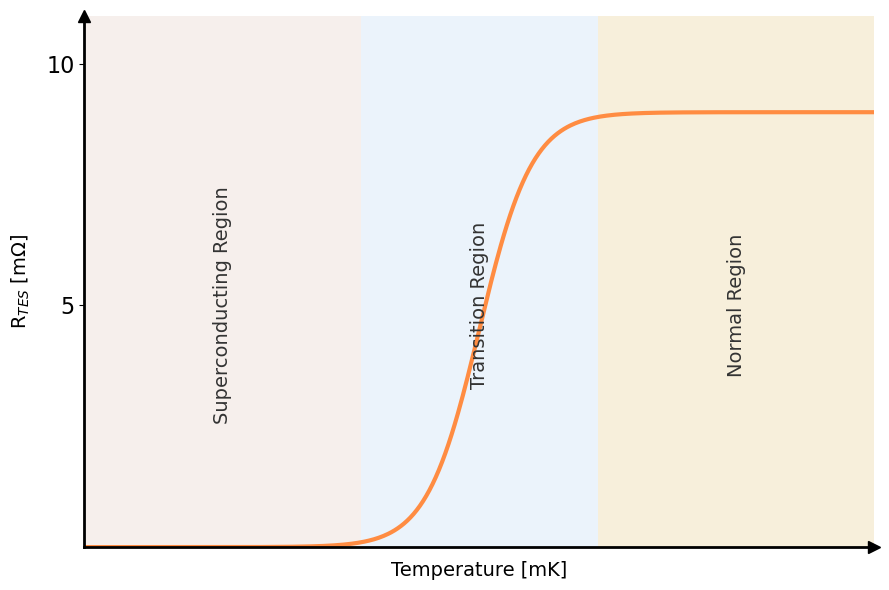
\includegraphics[width=0.7\textwidth]{figures/curva_transizione.png}
    \caption{Curva di transizione del TES. La resistenza passa rapidamente dallo stato superconduttore (R=0) allo stato normale (R=R$_n$) in un intervallo di temperatura molto ristretto.}
    \label{fig:tes_curve}
\end{figure}

Un secondo TES è posizionato sopra il light detector. Non potendo usare tubi fotomoltiplicatori per la rivelazione della luce, che introdurrebbero una quantità di radioattività intrinseca inaccettabile, nelle immediate vicinanze del cristallo di $\text{CaWO}_4$ viene posizionato un disco sottilissimo di silicio (il light detector), che funge da rivelatore di luce. I fotoni di scintillazione prodotti nel cristallo vengono assorbiti dal disco, generando fononi non termici che vengono rilevati dal TES sovrastante. L'apparato sperimentale è illustrato in figura \ref{fig:detector_module}.
\begin{figure}
    \centering
    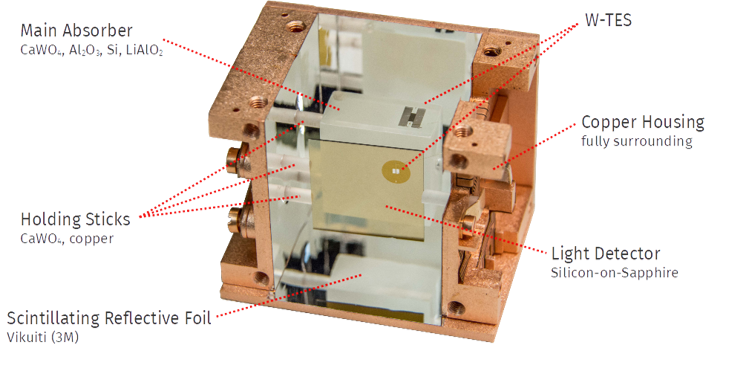
\includegraphics[width=0.7\textwidth]{figures/Detector_simple.png}
    \caption{Schema di un modulo rivelatore CRESST. Immagine tratta da \cite{cresst_detectors_2026}.}
    \label{fig:detector_module}
\end{figure}

Quando il cristallo viene colpito da una particella, il TES si scalda in tempi dell'ordine del millisecondo. Per poter registrare un evento successivo è necessario attendere che il sensore si raffreddi e torni alle condizioni di lavoro iniziali, un processo che avviene tipicamente in qualche decina di millisecondi (10-50~ms). Questo rapido ritorno all'equilibrio è possibile poiché all'aumentare della temperatura del TES, la sua resistenza elettrica subisce un brusco incremento che fa diminuire la corrente. Di conseguenza, la potenza dissipata per effetto Joule ($P = V^2/R$) si riduce, accelerandone il raffreddamento.

\subsubsection{Lo SQUID}

La variazione di corrente $\Delta I$ indotta nel TES dal passaggio di una particella è un segnale infinitesimo, dell'ordine dei nanoampere, che non potrebbe essere trasportato fino all'elettronica a temperatura ambiente tramite cavi convenzionali senza essere completamente sommerso dal rumore termico e dalle interferenze. Per ovviare a questo problema, la catena di lettura di CRESST introduce lo SQUID (\textit{Superconducting Quantum Interference Device}).


Come illustrato nello schema di Figura~\ref{fig:squid_circuit}, il circuito di bias del TES è connesso in parallelo ad un'induttanza. Quando un evento termico nel cristallo fa crescere la resistenza del TES, una maggior quantità di corrente viene deviata verso l'induttanza. Questa corrente genera un campo magnetico proporzionale che concatena l'anello dello SQUID.

\begin{figure}[htbp]
    \centering
    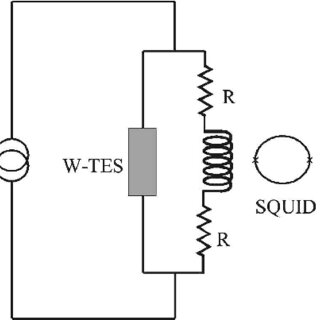
\includegraphics[width=0.45\textwidth]{figures/Readout-circuit-for-the-superconducting-thermometer-TES_Q320.jpg}
    \caption{Schema elettrico semplificato del circuito di lettura. La variazione di resistenza del TES modifica la ripartizione della corrente, che si traduce in un campo magnetico che concatena l'anello dello SQUID.}
    \label{fig:squid_circuit}
\end{figure}

Lo SQUID converte questo infinitesimo flusso magnetico in una variazione di tensione elettrica ($\Delta V$) misurabile dall'elettronica a temperatura ambiente. Offrendo un guadagno eccezionale e un rumore intrinseco virtualmente nullo, questo sistema permette di preservare e digitalizzare l'informazione sul rilascio energetico originario anche per eventi estremamente deboli, inferiori al $\text{keV}$.

\subsection{Il sistema di refrigerazione: il criostato a diluizione}
\label{subsec:criostato}

Per mantenere i moduli rivelatori, i TES e gli SQUID alla temperatura di lavoro millikelvin ($10\text{ mK}$) richiesta dall'esperimento, è necessario un sistema di refrigerazione sofisticato, capace di abbattere la temperatura di oltre cinque ordini di grandezza rispetto all'ambiente esterno. Questo compito è affidato a un criostato a diluizione di idrossido di elio ($^3\text{He}/^4\text{He}$), che opera attraverso una serie di stadi di raffreddamento progressivi:

\begin{enumerate}
    \item \textbf{Primo stadio (Pre-raffreddamento a $\sim 77\text{ K}$):} Il primo abbattimento termico massivo sfrutta il potere refrigerante dell'azoto liquido. Questo stadio riduce la temperatura del nucleo interno del criostato da temperatura ambiente fino a circa $77\text{ K}$ (temperatura di ebollizione dell'azoto), fungendo al contempo da prima barriera termica contro l'irraggiamento esterno.
    
    \item \textbf{Secondo stadio (Fase dell'Elio liquido a $\sim 4.2\text{ K}$ e $\sim 1\text{ K}$):} Il sistema viene successivamente raffreddato sfruttando le proprietà termiche dell'Elio liquido ($^4\text{He}$). A pressione atmosferica, l'elio bolle a $4.2\text{ K}$. Attraverso un sofisticato sistema di vuoto forzato è possibile abbassare ulteriormente la temperatura di ebollizione, spingendo questo stadio fino a circa $1\text{ K}$.
    
    \item \textbf{Terzo stadio (Unità a diluizione a $\sim 10\text{ mK}$):} Per scendere sotto la barriera di $1\text{ K}$ è necessario sfruttare le proprietà termodinamiche della miscela di due isotopi stabili dell'elio: l'Elio-3 ($^3\text{He}$) e l'Elio-4 ($^4\text{He}$). Quando questa miscela viene raffreddata sotto gli $0.8\text{ K}$, essa subisce una separazione spontanea in due fasi distinte: una fase "ricca" di $^3\text{He}$ (più leggera, che galleggia sopra) e una fase "diluita" (costituita quasi interamente da $^4\text{He}$ superfluido, in cui è disciolta una piccola frazione di $^3\text{He}$). 
\end{enumerate}

Tramite un sistema di pompaggio, gli atomi di $^3\text{He}$ vengono forzati ad attraversare la linea di separazione, passando dalla fase ricca alla fase diluita. Questo processo è endotermico: l'attraversamento della barriera richiede energia, che viene sottratta direttamente dall'ambiente circostante sotto forma di calore. È proprio grazie a questo continuo passaggio di fase quantistico che il criostato riesce ad assorbire il calore residuo dei rivelatori e a stabilizzare stabilmente l'intero apparato sperimentale alla temperatura criogenica di $10\text{ mK}$. Poiché questo meccanismo di raffreddamento utilizza materiali non radiopuri (serbatoi per l'azoto e l'elio, valvole e saldature etc...), il criostato deve stare al di fuori del modulo rivelatore. La temperatura criogenica è trasmessa al modulo tramite un collegamento in rame ultrapuro, che funge da ponte termico tra il criostato e il rivelatore come mostrato in Figura \ref{fig:shielding}.

\subsection{Discriminazione del fondo: il Light Yield}
\label{sec:light_yield}

Come introdotto nel paragrafo \ref{sec:doppio_canale} l'utilizzo di una tecnica a doppio canale (calore e luce) permette non solo di determinare l'energia totale rilasciata in un evento, ma anche di identificare la natura della particella interagente. Il parametro fondamentale per operare questa selezione dei dati è il \textit{Light Yield} ($LY$), definito come il rapporto tra l'energia misurata nel canale fotonico ($E_{\text{luce}}$) e l'energia totale depositata nel canale fononico ($E_{\text{calore}}$):

\begin{equation}
    LY = \frac{E_{\text{luce}}}{E_{\text{calore}}}
\end{equation}

La fisica alla base della discriminazione risiede nel fenomeno del \textit{quenching} della scintillazione: particelle ad alta densità di ionizzazione (come i nuclei di rinculo) perdono una frazione maggiore di energia in canali non radiativi rispetto a particelle a bassa densità di ionizzazione (come elettroni e fotoni). Di conseguenza, a parità di energia termica depositata nel cristallo ($E_{\text{calore}}$), un rinculo nucleare produrrà una quantità di luce significativamente inferiore rispetto a un rinculo elettronico, posizionandosi a valori di $LY$ decisamente più bassi.

Nel caso specifico dei cristalli di $\text{CaWO}_4$ impiegati in CRESST, il target è composto da tre diversi nuclei bersaglio (Calcio, Ossigeno e Tungsteno), ciascuno caratterizzato da un differente fattore di quenching dovuto alla diversa massa nucleare. Questa particolarità si traduce nella separazione dei dati in bande ben distinte all'interno del piano $LY$ in funzione dell'energia, come illustrato nella Figura~\ref{fig:bands}.

\begin{figure}[htbp]
    \centering
    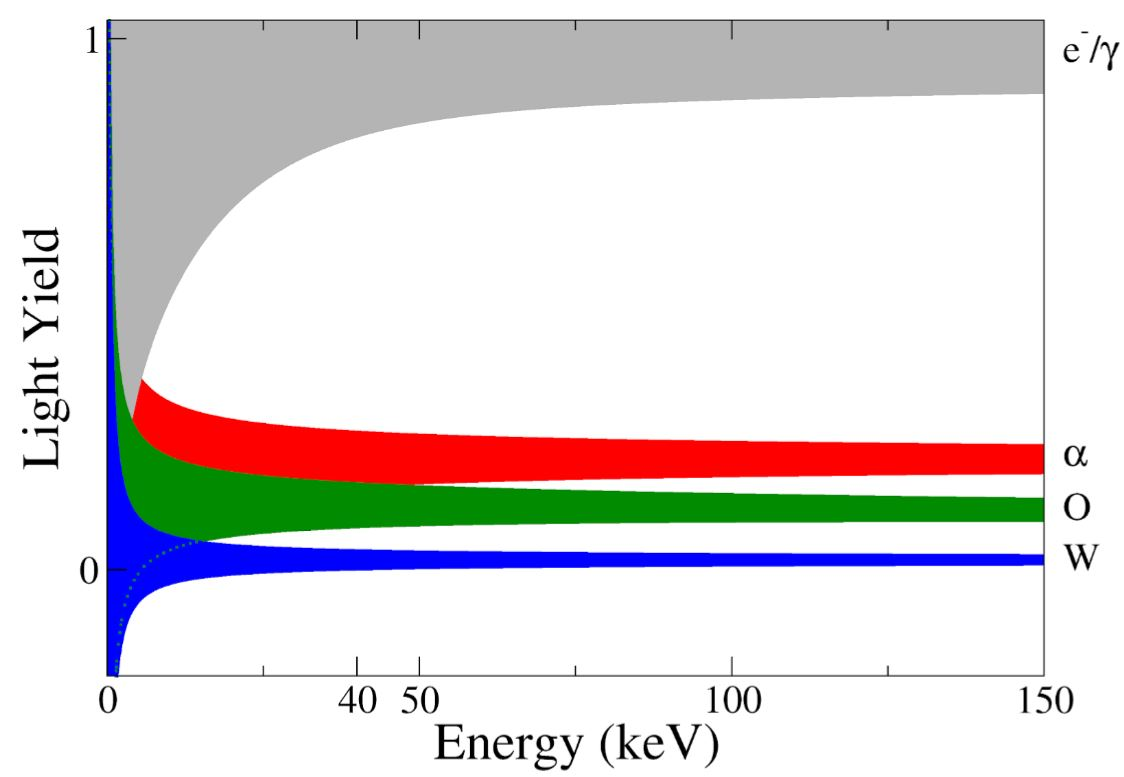
\includegraphics[width=0.85\textwidth]{figures/Bands.JPG}
    \caption{Rappresentazione schematica delle bande di evento nel piano Light Yield in funzione dell'energia per un cristallo di $\text{CaWO}_4$. Si distinguono nettamente la banda grigia superiore dei rinculi elettronici ($e^-/\gamma$) e le bande inferiori associate ai rinculi nucleari di alfa ($\alpha$), ossigeno (O) e tungsteno (W). La larghezza delle bande aumenta a basse energie a causa delle fluttuazioni statistiche nella raccolta dei fotoni. Immagine tratta da \cite{cresst_detectors_2026}.}
    \label{fig:bands}
\end{figure}

Analizzando la Figura~\ref{fig:bands}, è possibile identificare le diverse componenti che popolano il diagramma:
\begin{itemize}
    \item \textbf{Banda $e^-/\gamma$ (regione grigia):} Posizionata attorno a $LY \approx 1$, accoglie i rinculi elettronici derivanti dalla radioattività ambientale $\beta$ e $\gamma$. Rappresenta la quasi totalità del fondo sperimentale.
    \item \textbf{Banda $\alpha$ (regione rossa):} Dovuta a contaminazioni interne o superficiali di emettitori alfa.
    \item \textbf{Bande dei rinculi nucleari (regioni verde e blu):} I nuclei di Ossigeno (O) e Tungsteno (W) mostrano un quenching progressivamente più marcato a causa della loro maggiore massa. Una WIMP di materia oscura, interagendo prevalentemente tramite scattering coerente con i nuclei del bersaglio (con una sezione d'urto che scala come $A^2$, favorendo il Tungsteno pesante), produrrebbe eventi confinati principalmente nella banda del Tungsteno (W) o dell'Ossigeno (O).
\end{itemize}

\section{Scudi attivi e passivi}
\label{sec:scudi}

L'apparato sperimentale di CRESST è protetto da un sistema di schermatura a più livelli, progettato per ridurre al minimo il fondo sperimentale e massimizzare la sensibilità alla materia oscura. Questo sistema si compone di due componenti principali: scudi passivi e scudi attivi.

\begin{itemize}
    \item \textbf{scudi passivi:} materiali ad alta densità come piombo e rame, che circondano il criostato e i moduli rivelatori, assorbendo la radiazione ambientale $\gamma$ e riducendo la radioattività di fondo. Questi strati schermano efficacemente i raggi cosmici e le particelle cariche provenienti dall'ambiente esterno.
    \item \textbf{scudi attivi:} un sistema di scintillatori viene utilizzato per rilevare i muoni cosmici residui ed eliminarli \textit{a posteriori}.
\end{itemize}

In particolare l'articolata successione di scudi passivi, rappresentata in Figura \ref{fig:shielding}, dall'esterno all'interno consta di:

\begin{wrapfigure}{r}{0.45\textwidth}
    \centering
    \vspace{-20pt} % Riduce lo spazio bianco sopra la figura per allinearla al testo
    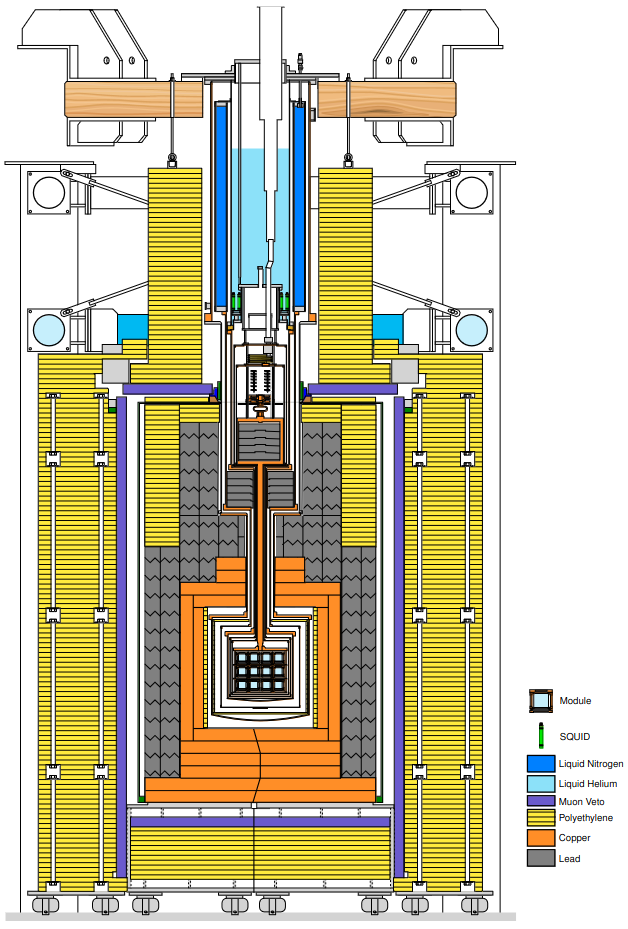
\includegraphics[width=0.42\textwidth]{figures/Schematic-cross-section-of-the-CRESST-setup-27-showing-the-structure-of-the-cryostat.ppm.png}
    \caption{Schema del sistema di schermatura di CRESST.}
    \label{fig:shielding}
    \vspace{-10pt} % Riduce lo spazio bianco sotto la didascalia
\end{wrapfigure}

\begin{enumerate}
    \item uno spesso strato di polietilene (\SI{40}{\cm}), che funge da moderatore per i neutroni ambientali. Grazie alla composizione chimica ricca di idrogeno, il polietilene rallenta i neutroni veloci, riducendo la loro energia fino a valori termici, per poi essere catturati tramite cattura radiativa.
    \item uno strato di piombo di circa \SI{20}{\cm}, che riduce la radioattività ambientale $\gamma$. Poiché il piombo è leggermente radioattivo, a causa della presenza di $^{210}\text{Pb}$, si utilizza piombo o a basso contenuto di questo isotopo, o piombo antico, che ha avuto il tempo di decadere.
    \item uno strato di rame di circa \SI{14}{\cm} estremamente radiopuro, che funge da ultima barriera e riduce al minimo il rumore di fondo.
\end{enumerate}

Inoltre, in Figura \ref{fig:shielding} è rappresentato uno spessore viola associato al termine "muon veto". Questo scudo rappresenta l'ultimo metodo (attivo) di schermaggio contro i muoni cosmici residui. Essendo sotto \SI{1400}{\metre} di roccia, il flusso di muoni cosmici è ridotto di circa sei ordini di grandezza rispetto alla superficie terrestre, raggiungendo un valore di $1$ muone al metro quadro ogni ora, che rischierebbe di contaminare eccessivamente il segnale di materia oscura. 

Per questo motivo viene installato un sistema di scintillatori plastici che, colpiti da un muone, si eccitano, per poi tornare allo stato fondamentale emettendo fotoni di scintillazione, raccolti da tubi fotomoltiplicatori. Quando i fotomoltiplicatori registrano il passaggio di un muone e viene contemporaneamente rilevato un evento nel cristallo, esso viene scartato, poiché non dovuto a materia oscura.
 %2 
\clearpage{\thispagestyle{empty}\cleardoublepage}
\chapter{Costruzione dell'Optimum Filter e Caratterizzazione del Rumore}
\label{ch:OF}

Negli esperimenti di ricerca diretta di materia oscura come CRESST, la rivelazione di eventi rari e a bassissimo rilascio energetico impone di massimizzare il rapporto segnale-rumore (\textit{Signal-to-Noise Ratio}, SNR). Ottimizzare questo parametro consente di ridurre la soglia energetica del rivelatore ($E_{\text{th}}$), garantendo al tempo stesso un'elevata efficienza di selezione dei segnali fisici e un forte rigetto dei trigger spuri dovuti a fluttuazioni termiche ed elettroniche.

Questo capitolo descrive il percorso adottato per il trattamento dei dati: dalla struttura dei campioni registrati alla formulazione teorica dell'\textit{Optimum Filter} (OF), fino alla determinazione dei suoi due elementi costitutivi — il \textit{Noise Power Spectrum} (NPS) e i template di forma d'onda. Infine (forse), viene presentata l'applicazione del filtro e il criterio di stima del tasso di rumore triggerato in funzione della soglia.

% ==============================================================================
\section{Struttura dei Dati e Parametrizzazione delle Tracce}
\label{sec:struttura_dati}
% ==============================================================================

Nell'esperimento CRESST i segnali vengono acquisiti in modalità continua a una frequenza di campionamento di $25\,\text{kHz}$, che corrisponde a un intervallo temporale tra due campioni consecutivi pari a $\Delta t = 40\,\mu\text{s}$. La registrazione continua consente di applicare algoritmi di filtraggio digitale direttamente sul flusso dati grezzo, per poi applicare in un secondo momento il trigger, riducendo l'impatto del rumore e migliorando la sensibilità sperimentale.

Per monitorare la stabilità della risposta termica del rivelatore e verificarne costantemente il punto di lavoro lungo la transizione superconduttrice del TES (\textit{Transition Edge Sensor}), vengono iniettati periodicamente impulsi di calore artificiali per mezzo di un riscaldatore ohmico (\textit{heater}) integrato sull'assorbitore:
\begin{itemize}
    \item \textbf{TestPulses:} impulsi di calore ad ampiezza variabile programmata (tra $0.1\,\text{V}$ a $10\,\text{V}$ al generatore), impiegati per campionare linearità, guadagno e risoluzione energetica dell'apparato (Figura~\ref{fig:PulsesComparison}b);
    \item \textbf{ControlPulses:} impulsi ad ampiezza fissa ed elevata ($20\,\text{V}$), progettati per portare il film di tungsteno oltre la transizione e saturare la risposta (Figura~\ref{fig:PulsesComparison}a). L'altezza del gradino di saturazione funge da riferimento stabile per correggere eventuali derive termiche del criostato. (Il controlpulse sembra avere stessa ampiezza dell'ultimo Testpulse nonostante ampiezza input registrata sia doppia!!!!)
\end{itemize}

\begin{figure}[htbp]
    \centering
    \begin{minipage}[t]{0.48\textwidth}
        \centering
        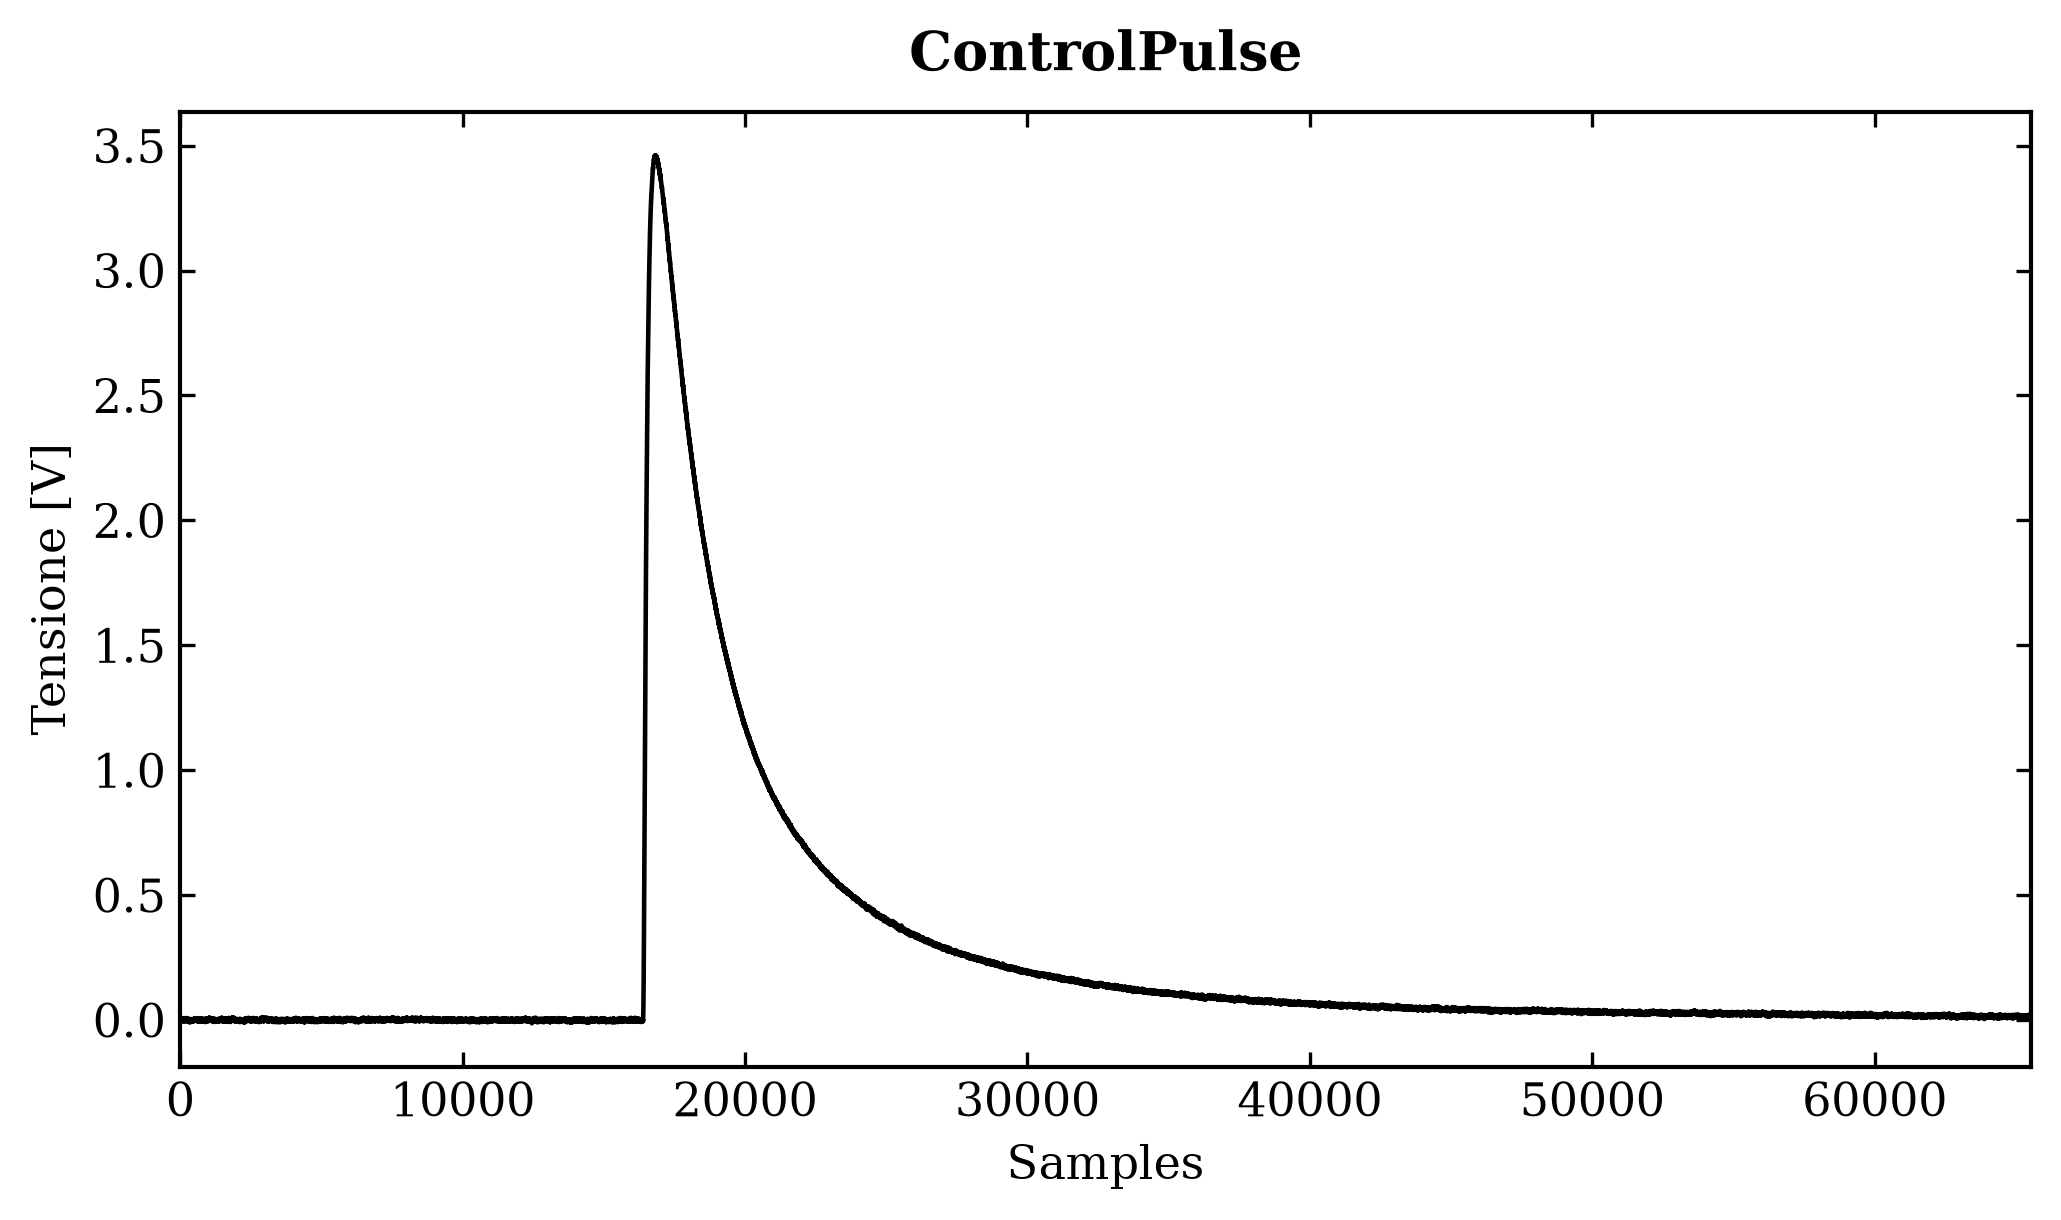
\includegraphics[width=\linewidth]{figures/ControlPulse.png}
        \caption*{(a) Impulso a 20\,V (ControlPulse).}
        \label{fig:ControlPulse}
    \end{minipage}
    \hfill
    \begin{minipage}[t]{0.48\textwidth}
        \centering
        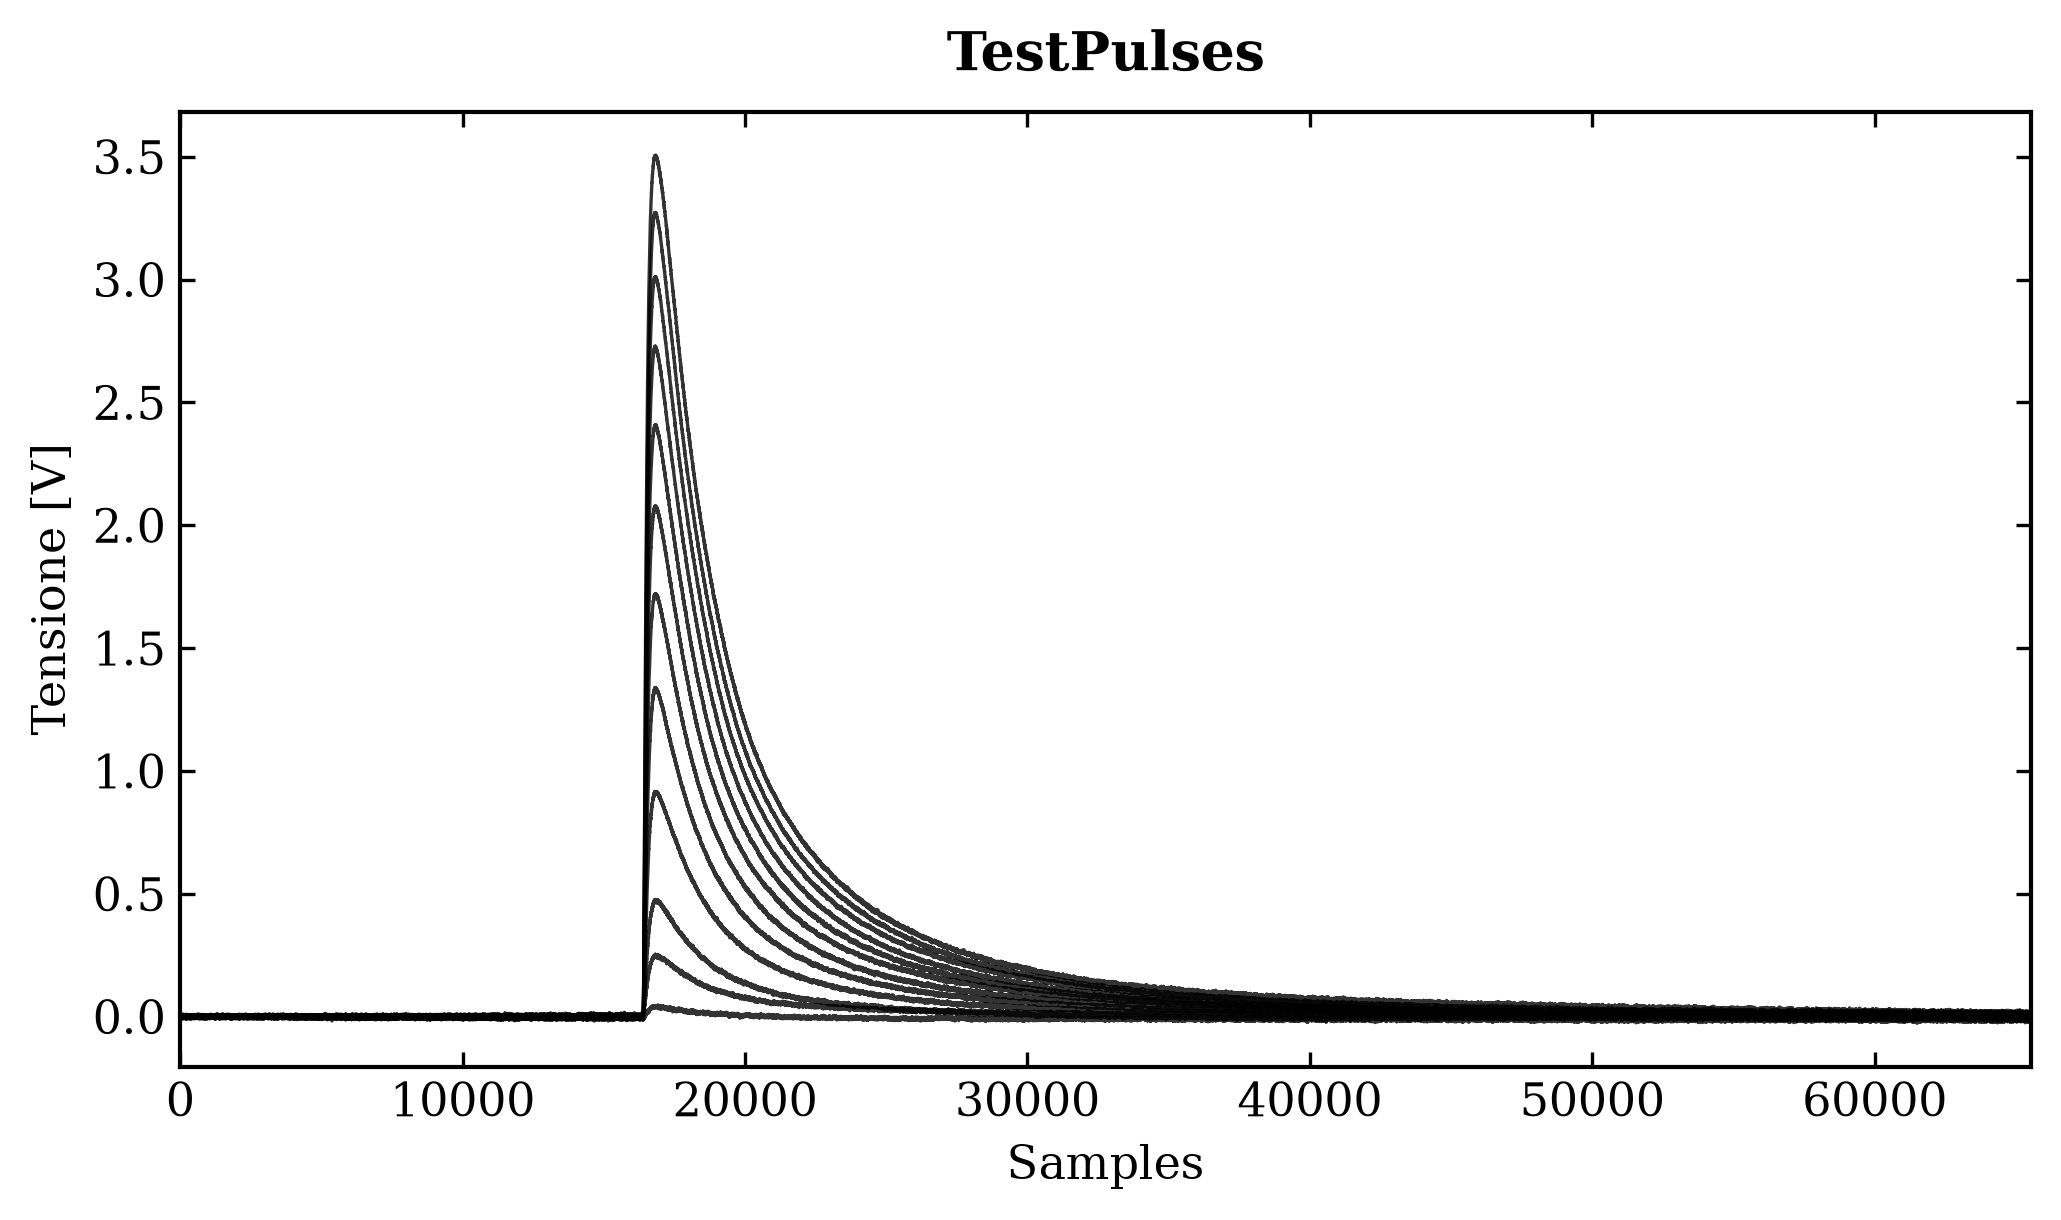
\includegraphics[width=\linewidth]{figures/testpulse.png}
        \caption*{(b) Impulsi tra 0.1\,V e 10\,V (TestPulses).}
        \label{fig:TestPulse}
    \end{minipage}
    \vspace{0.8em}
    \caption{Risposta del sensore agli impulsi iniettati tramite heater: (a) singolo \textit{ControlPulse} saturo a $20\,\text{V}$ e (b) serie di dodici \textit{TestPulses} ad ampiezza variabile campionati lungo l'intervallo di 65536 campioni.}
    \label{fig:PulsesComparison}
\end{figure}

Ogni evento isolato in fase di analisi corrisponde a una finestra temporale di $65536$ campioni (durata complessiva di circa $2.62\,\text{s}$). L'impulso viene convenzionalmente posizionato a un quarto della traccia, attorno al campione $16384$ ($\approx 655.4\,\text{ms}$). Questa asimmetria garantisce un intervallo pre-trigger sufficientemente lungo per stimare il livello e la varianza della linea di base (\textit{baseline}), lasciando al contempo il tempo necessario per registrare il completo rilassamento termico del sistema verso il bagno freddo.

Dalle tracce campionate vengono estratti diversi parametri operativi, riassunti nel seguente elenco e illustrati in Figura~\ref{fig:Parametri_particella}:
\begin{itemize}
    \item \textbf{Baseline Offset:} valore medio della tensione nella finestra pre-trigger, sottratto alla traccia per eliminare la componente continua (DC);
    \item \textbf{Baseline Slope:} pendenza lineare della baseline pre-trigger (unità di misura??);
    \item \textbf{Baseline RMS:} deviazione standard della tensione nella regione prima dell'evento;
    \item \textbf{Baseline Difference:} differenza tra la media della tensione prima dell'impulso e quella a fine finestra;
    \item \textbf{Rise Time (RT):} tempo impiegato dal fronte di salita per passare dal $x\%$ al $x\%$ dell'altezza massima;
    \item \textbf{Decay Time (DT):} tempo impiegato dalla coda del segnale per scendere dal $x\%$ al $x\%$ del picco;
    \item \textbf{Peak Position:} coordinata temporale del massimo assoluto identificato lungo la finestra.
\end{itemize}

\begin{figure}[htbp]
    \centering
    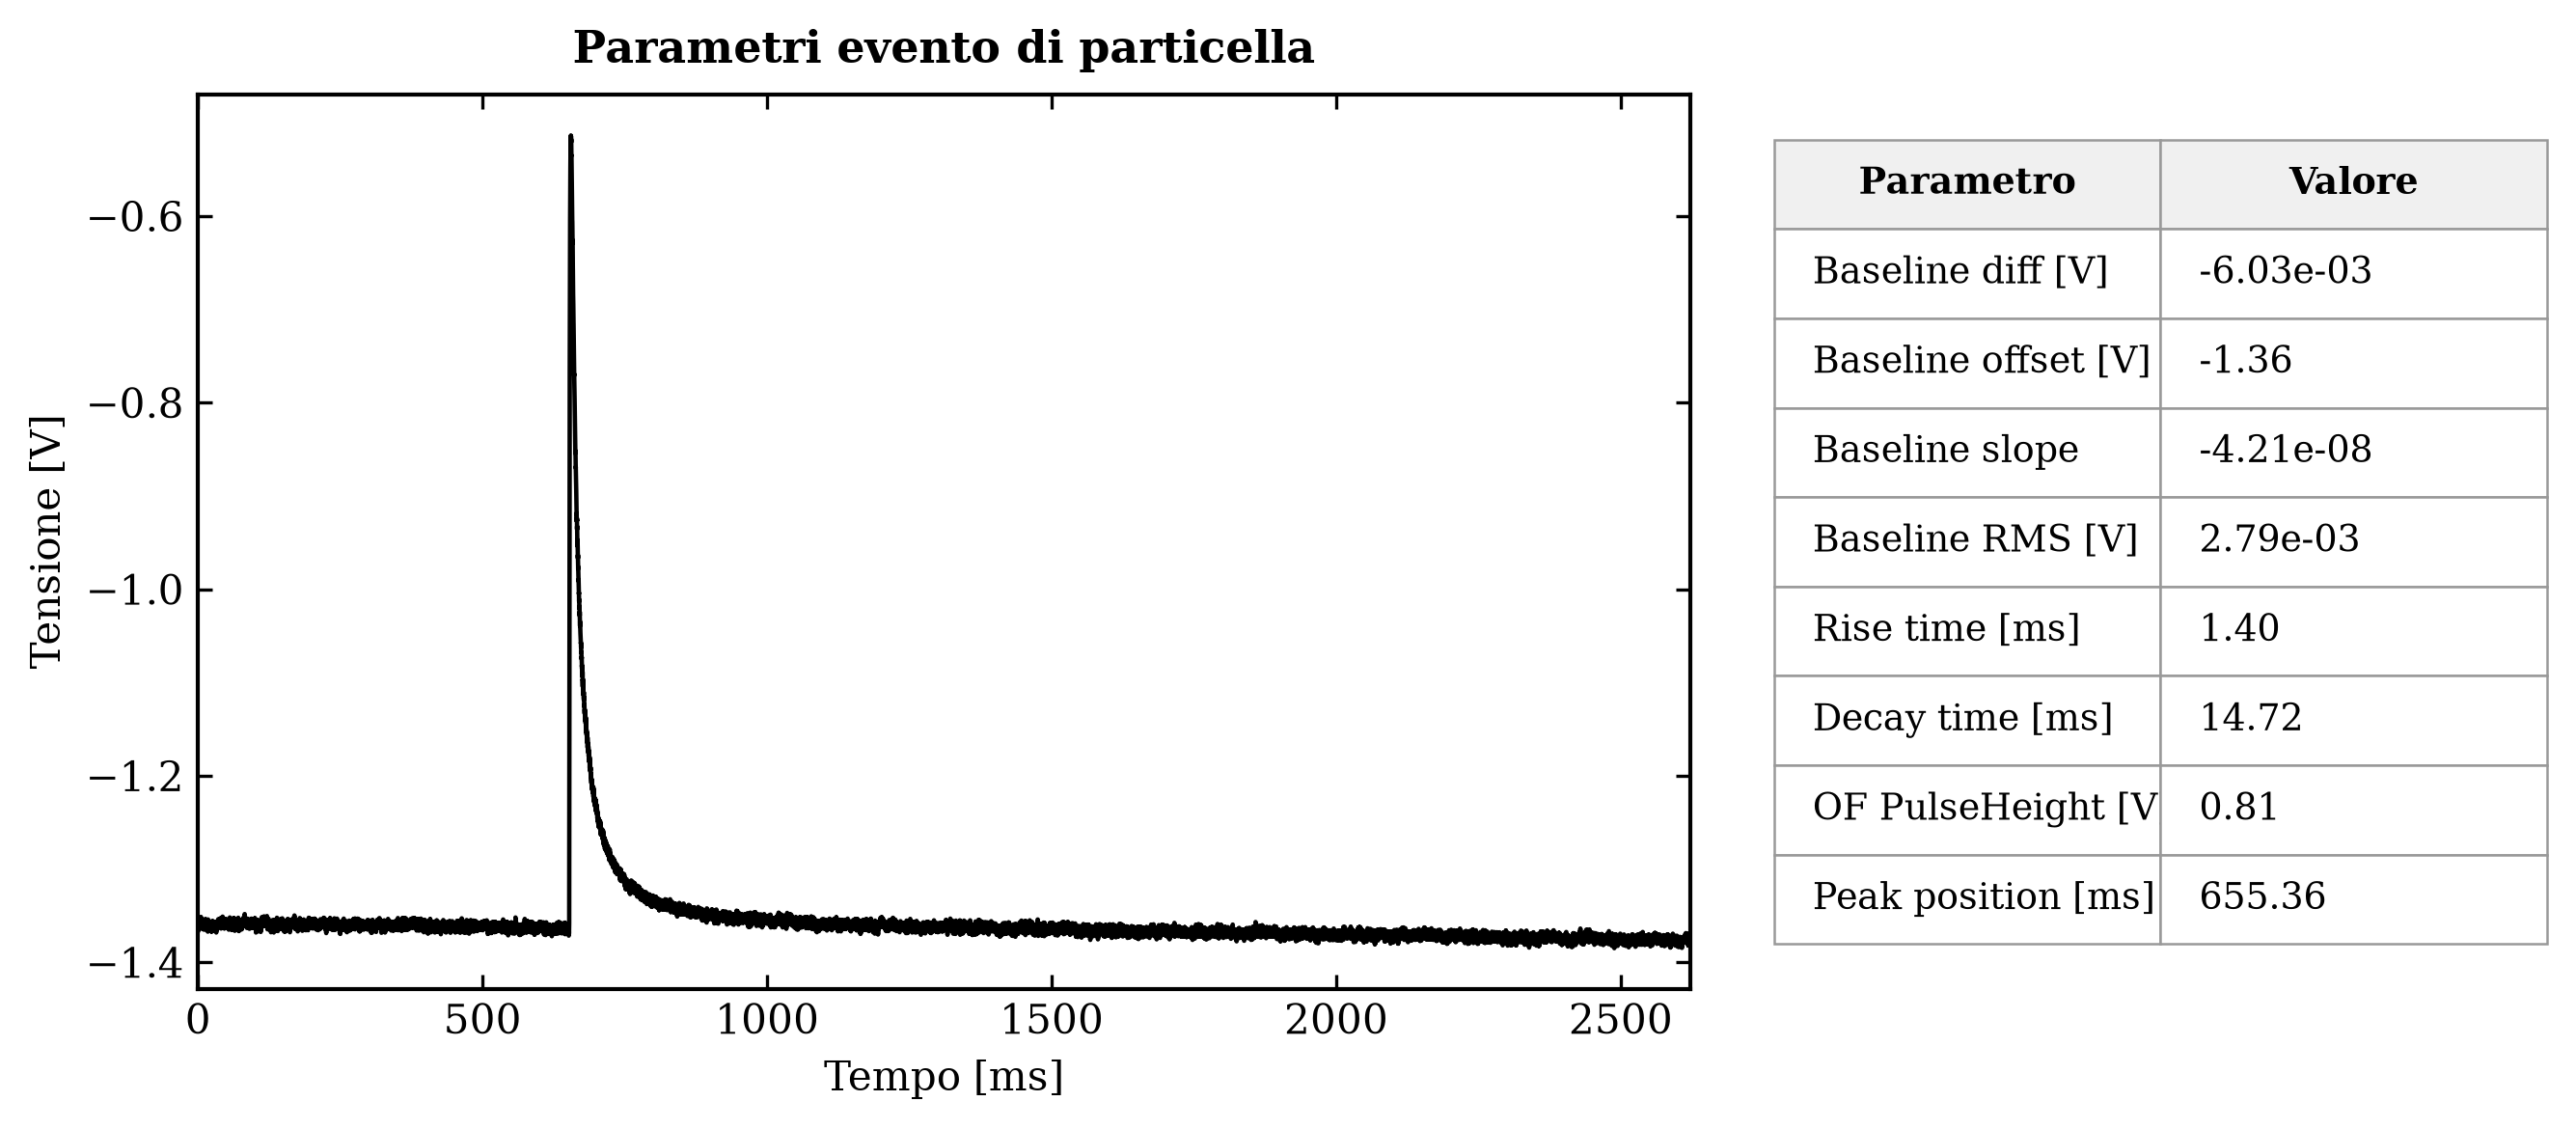
\includegraphics[width=0.95\textwidth]{figures/Parametri_particella.png}
    \caption{Esempio di traccia di particella registrata nel cristallo (a sinistra) e relativa tabella dei parametri di forma calcolati (a destra). (Sistemare unità di misura!!!!)}
    \label{fig:Parametri_particella}
\end{figure}

% ==============================================================================
\section{Formalismo Teorico dell'Optimum Filter}
\label{sec:teoria_OF}
% ==============================================================================

Il metodo più immediato per ricavare l'energia depositata da un'interazione consisterebbe nel campionare il valore massimo della traccia dopo aver rimosso l'offset della baseline. Tuttavia, in presenza di segnali di piccola ampiezza confrontabili con l'RMS del fondo, il massimo misurato tende a coincidere con la somma tra l'impulso reale e la più alta fluttuazione casuale positiva presente in quel punto. Questo effetto introduce una sovrastima sistematica dell'ampiezza.

Per ovviare al problema si adotta l'\textit{Optimum Filter} (OF), sviluppato originariamente da Gatti e Manfredi ~\cite{gatti_manfredi}. L'algoritmo sfrutta il fatto che, in regime di risposta lineare del sensore, gli impulsi condividono una forma d'onda comune e differiscono unicamente per un fattore di scala proporzionale all'energia. Una traccia misurata $v(t)$, depurata dall'offset continuo, viene quindi modellata come:
\begin{equation}
    v(t) = A \cdot s(t - t_0) + n(t)
    \label{eq:segnale_modello}
\end{equation}
dove $s(t)$ è la forma d'onda attesa normalizzata a massimo unitario (\textit{template}), $A$ è l'ampiezza incognita da stimare, $t_0$ è l'istante di arrivo del segnale ed $n(t)$ è il rumore stocastico additivo sovrapposto.

L'Optimum Filter opera nello spazio delle frequenze tramite una funzione di trasferimento $H(f)$ costruita per massimizzare il rapporto tra l'ampiezza dell'impulso e il rumore di fondo. Tale funzione assume la forma:
\begin{equation}
    H(f) = K \frac{S^*(f)}{N(f)} e^{-i 2\pi f t_0}
    \label{eq:OF_transfer_function}
\end{equation}
dove:
\begin{itemize}
    \item $S^*(f)$ è il complesso coniugato della trasformata di Fourier del template $s(t)$, che pesa maggiormente le bande di frequenza in cui si concentra la potenza del segnale fisico;
    \item $N(f)$ è la densità di potenza del rumore (\textit{Noise Power Spectrum}, NPS), che ha il compito di ridurre le frequenze dominate da disturbi sperimentali;
    \item $e^{-i 2\pi f t_0}$ compensa lo sfasamento temporale dell'evento lungo la traccia;
    \item $K$ è una costante reale di normalizzazione definita come:
    \begin{equation}
        K = \left( \int_{-\infty}^{+\infty} \frac{|S(f)|^2}{N(f)} \, df \right)^{-1}
        \label{eq:costante_normalizzazione}
    \end{equation}
    Poiché i segnali sperimentali vengono acquisiti a tempo discreto su un intervallo finito di $N$ campioni, l'integrale viene valutato numericamente tramite sommatoria sui bin di frequenza discreti $f_k = k \cdot \Delta f$ (con $\Delta f = f_camp / N$). Sfruttando la proprietà per cui il modulo quadro della trasformata di Fourier di un segnale reale è una funzione pari rispetto all'origine ($|S(-f)|^2 = |S(f)|^2$), l'integrazione sulle frequenze negative si ripiega su quelle positive:
    \begin{equation}
        K = \left[ \Delta f \left( \frac{|S(0)|^2}{N(0)} + 2 \sum_{k=1}^{N/2 - 1} \frac{|S(f_k)|^2}{N(f_k)} + \frac{|S(f_{\text{Nyq}})|^2}{N(f_{\text{Nyq}})} \right) \right]^{-1}
        \label{eq:costante_normalizzazione_discreta}
    \end{equation}
dove $f_{\text{Nyq}} = f_{N/2} = f_s / 2$ rappresenta la frequenza di Nyquist, che, insieme alla componente continua ($k=0$), è l'unica a comparire con peso unitario in quanto non possiedono una controparte simmetrica nell'intervallo fondamentale.
\end{itemize}

Una volta calcolata $H(f)$, la traccia filtrata nel tempo si ottiene applicando l'antitrasformata di Fourier al prodotto tra lo spettro del segnale grezzo $V(f)$ e il filtro:
\begin{equation}
    v_{\text{filt}}(t) = \mathcal{F}^{-1} \Big[ V(f) \cdot H(f) \Big]
\end{equation}
Il massimo di $v_{\text{filt}}(t)$ fornisce la stima ottimale dell'ampiezza cercata ${A}$ (\ref{eq:segnale_modello}), indicata come \textit{Optimum Filter Pulse Height}, mentre l'istante in cui cade tale picco identifica il parametro \textit{Peak Position}.

% ==============================================================================
\section{Caratterizzazione del Rumore e Stima del Noise Power Spectrum}
\label{sec:costruzione_NPS}
% ==============================================================================

Per calcolare il denominatore della funzione di trasferimento dell'OF è necessario stimare sperimentalmente la densità spettrale $N(f)$ a partire da finestre temporali registrate in assenza di segnale fisico.

Durante il funzionamento continuo, le inevitabili derive termiche a bassissima frequenza dell'apparato criogenico provocano variazioni della linea di base. Se una finestra di rumore presenta una deriva non nulla, i livelli di tensione all'inizio e alla fine risulteranno disallineati. Poiché la Trasformata Discreta di Fourier (DFT) tratta implicitamente il record come una sequenza periodica, il disallineamento tra i due estremi viene interpretato come una discontinuità a gradino. Tale gradino introduce una forte componente spuria a bassa frequenza, che distorce e sovrastima lo spettro del rumore, come illustrato in Figura~\ref{fig:gradino}.

\begin{figure}[htbp]
    \centering
    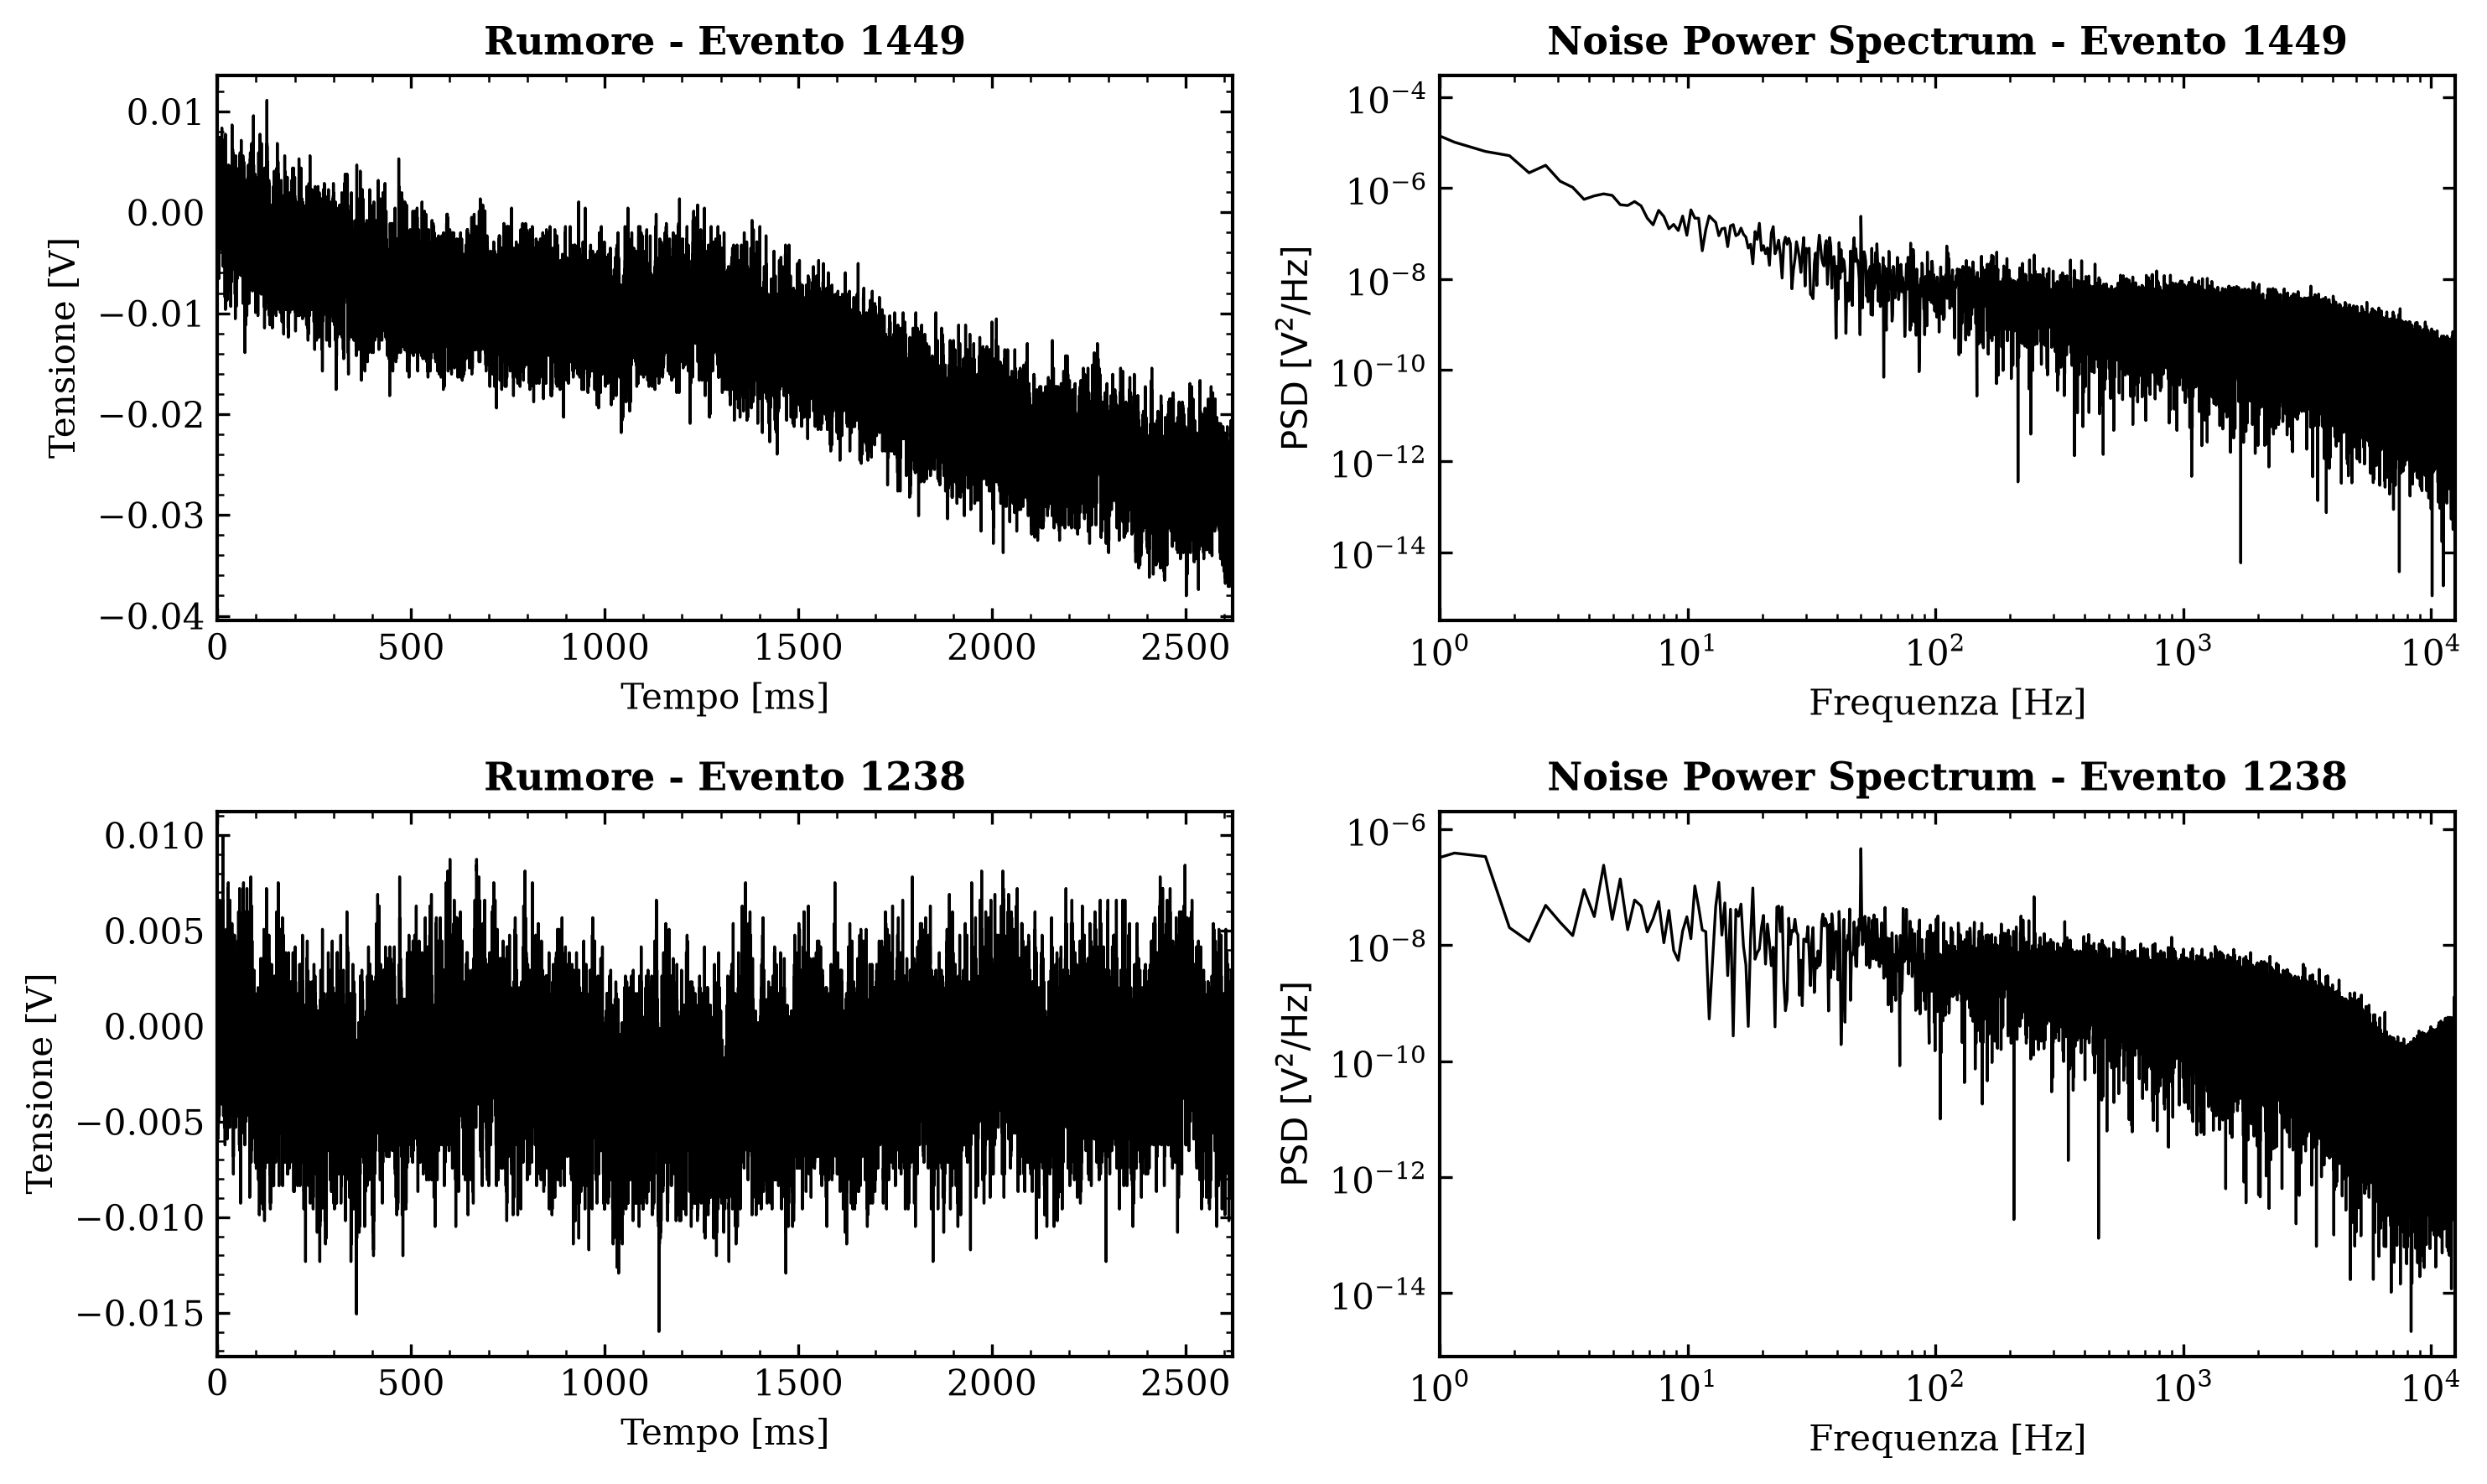
\includegraphics[width=0.9\textwidth]{figures/NPS_baselines.png}
    \caption{Confronto tra due tracce di rumore: l'evento superiore risente di una deriva di baseline che produce un gradino tra i margini, generando nello spettro un'iniezione fittizia di potenza a bassa frequenza; l'evento inferiore, piatto e stazionario, restituisce il profilo indisturbato del rumore.}
    \label{fig:gradino}
\end{figure}

Per selezionare esclusivamente tracce di rumore stazionarie, il campione iniziale viene depurato applicando una serie di criteri di selezione:
\begin{itemize}
    \item \textbf{Pulse Height $< 4\,\text{mV}$:} esclude piccoli impulsi fisici o transienti spuri sfuggiti al trigger;
    \item \textbf{Baseline Difference $< 0.5\,\text{mV}$:} rigetta eventi che contengono code termiche o fluttuazioni a gradino;
    \item \textbf{Fit polinomiale di terzo grado:} la traccia viene modellata con un polinomio cubico. Si conservano solo gli eventi con coefficienti compresi tra il $10^\circ$ e il $90^\circ$ percentile della distribuzione, eliminando andamenti non lineari anomali.
\end{itemize}

Sulle tracce accettate si sottrae il fit cubico per rimuovere ogni pendenza residua (\textit{detrending}). Si calcola quindi la trasformata $V_i(f)$ per ciascuna delle $M$ tracce selezionate e si valuta la Densità Spettrale di Potenza a frequenze positive:
\begin{equation}
    N(f) = \frac{2}{N f_s} \frac{1}{M} \sum_{i=1}^{M} |V_i(f)|^2
\end{equation}
dove $N = 65536$ è il numero di campioni, $f_s = 25\,\text{kHz}$ è la frequenza di campionamento e il fattore 2 preserva la potenza totale piegando le frequenze negative su quelle positive.

\begin{figure}[htbp]
    \centering
    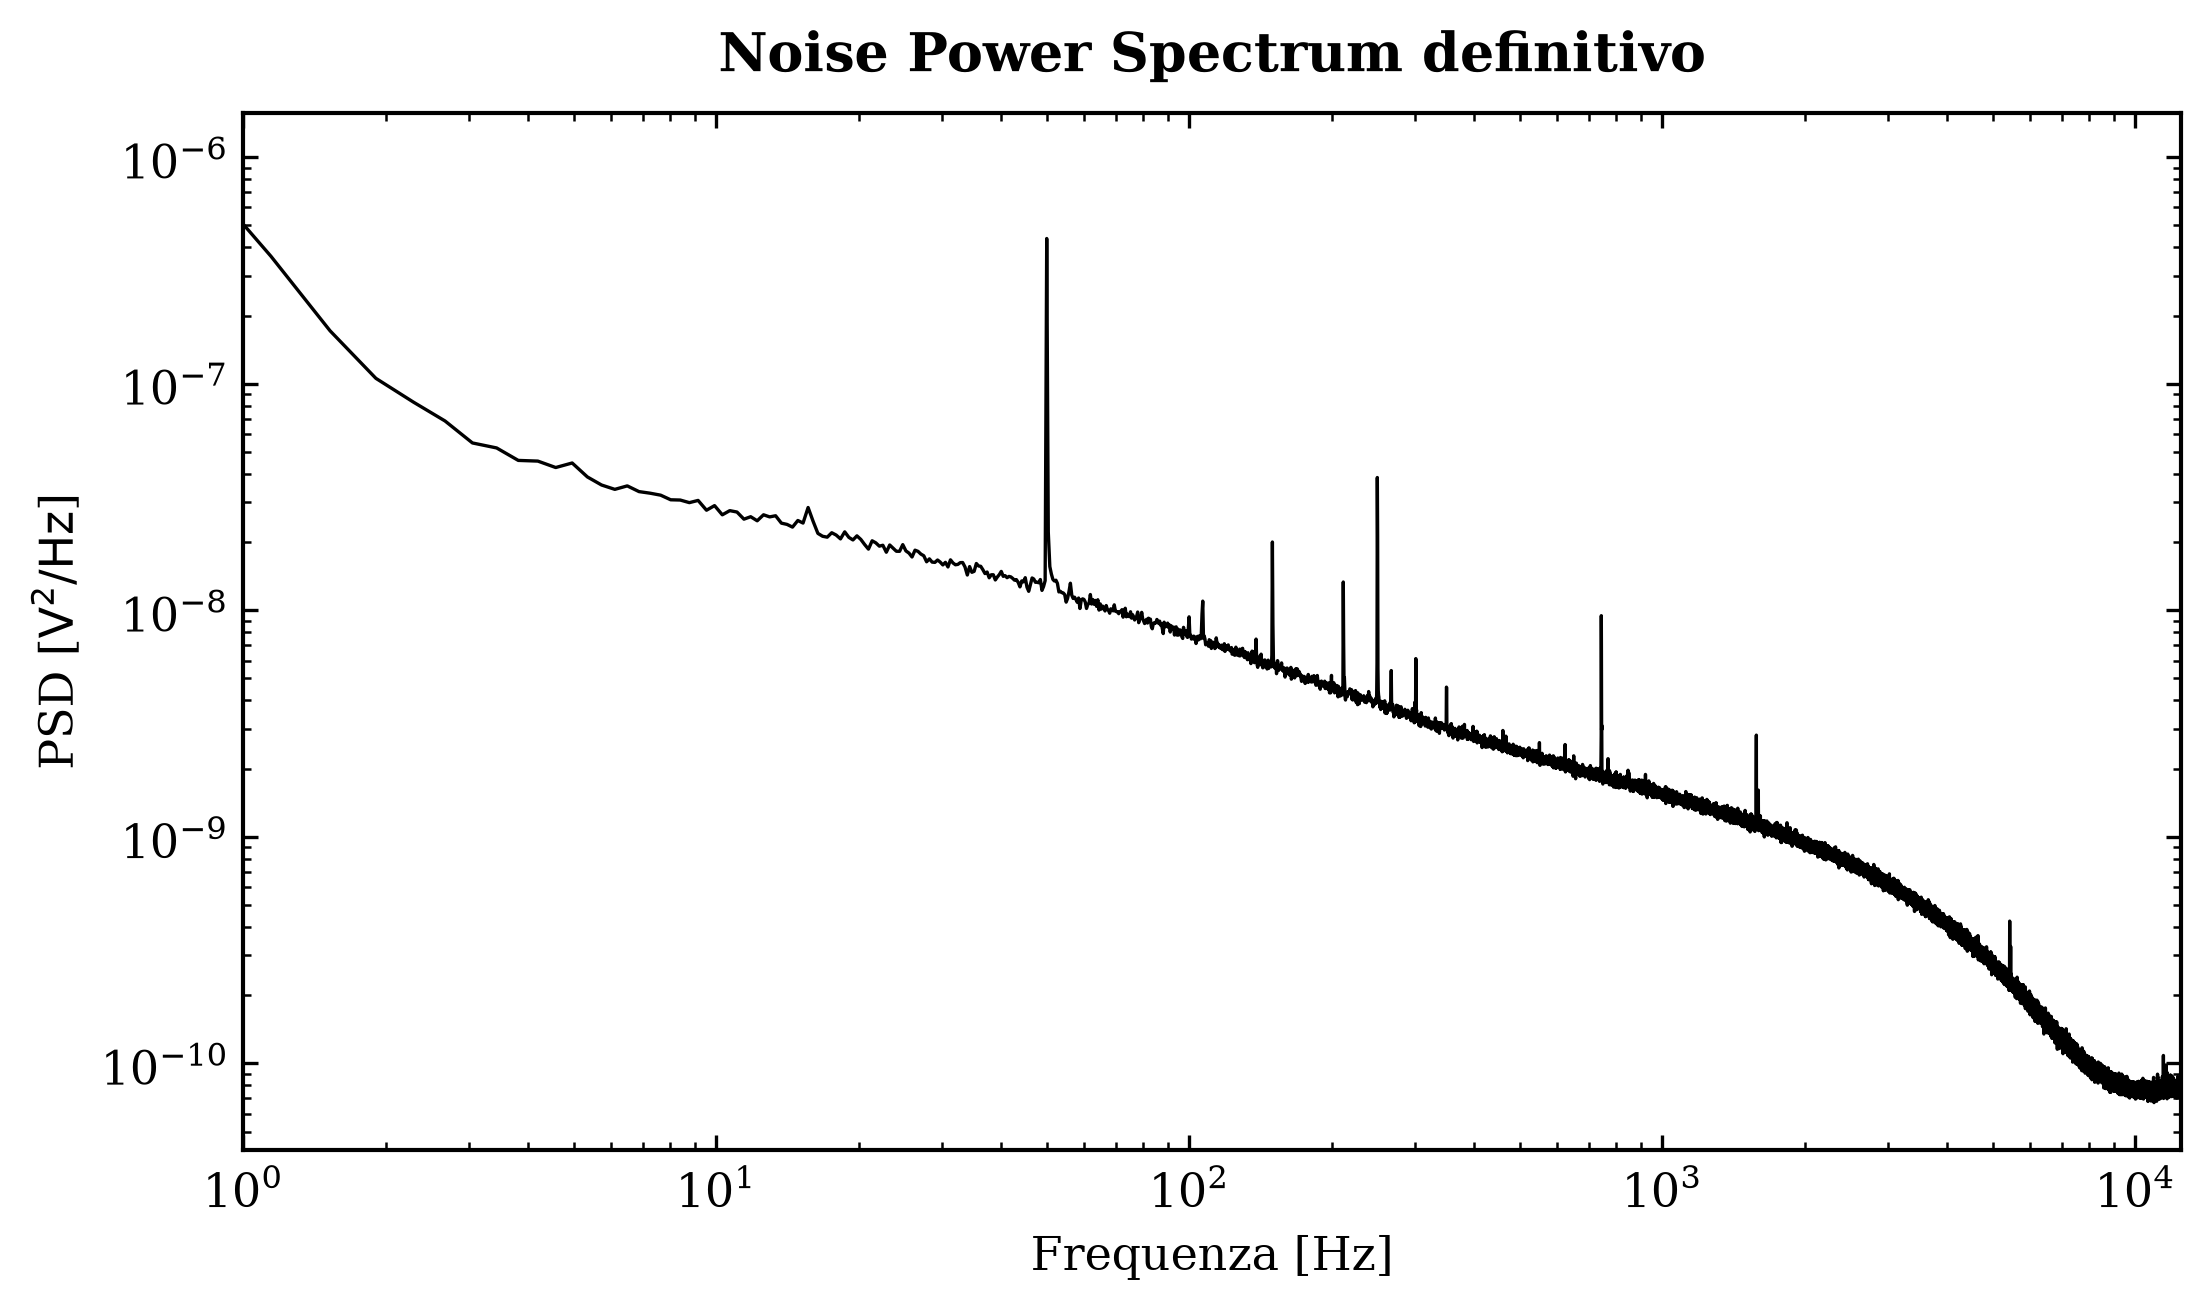
\includegraphics[width=0.9\textwidth]{figures/NPS.png}
    \caption{\textit{Noise Power Spectrum} ottenuto dalla media e normalizzazione di circa 1000 eventi di rumore depurati con fit di terzo grado.}
    \label{fig:NPS}
\end{figure}

Lo spettro finale (Figura~\ref{fig:NPS}) evidenzia chiaramente i contributi del rumore di fondo: oltre a una componente continua a bassa frequenza, emergono il picco fondamentale della rete a $50\,\text{Hz}$ e le relative armoniche dispari ($150\,\text{Hz}$ e $250\,\text{Hz}$), dovute a captazioni elettromagnetiche e ground loop. Inserito a denominatore nella funzione di trasferimento $H(f)$, $N(f)$ smorza selettivamente queste frequenze, eliminando le interferenze periodiche dalla stima dell'ampiezza.

% ==============================================================================
\section{Costruzione dei Template di Segnale}
\label{sec:costruzione_template}
% ==============================================================================

Il numeratore dell'Optimum Filter richiede la conoscenza della forma d'onda di riferimento $s(t)$ (\ref{eq:segnale_modello}). Poiché i canali di eccitazione del rivelatore sono due, particelle ionizzanti che interagiscono nel volume del cristallo e impulsi termici iniettati sull'heater, è necessario definire due template separati.

% ------------------------------------------------------------------------------
\subsection{Template Fononico per Eventi Fisici}
\label{subsec:template_fononico}

Per ricavare il template del segnale particellare, l'obiettivo è mediare un insieme numericamente consistente di tracce pulite, in modo da cancellare il rumore stocastico e isolare la dinamica termica pura. 

A questo scopo sono stati selezionati eventi prodotti da una sorgente esterna di calibrazione di $^{55}\text{Fe}$. Il decadimento per cattura elettronica del $^{55}\text{Fe}$ genera raggi X caratteristici a circa $5.9\,\text{keV}$ ($K_\alpha$) e $6.4\,\text{keV}$ ($K_\beta$). Questa energia è ideale: è sufficientemente elevata da emergere nettamente dal rumore di fondo, ma abbastanza contenuta da non saturare il sensore TES, garantendo una risposta strettamente lineare.

Gli eventi vengono selezionati richiedendo una \textit{pulse height} preliminare compresa tra $0.8\,\text{V}$ e $0.9\,\text{V}$ (intervallo corrispondente al picco del ferro), assenza di derivate negative anomale (generate da disturbi dell'elettronica) e stabilità della linea di base.

\begin{figure}[htbp]
    \centering
    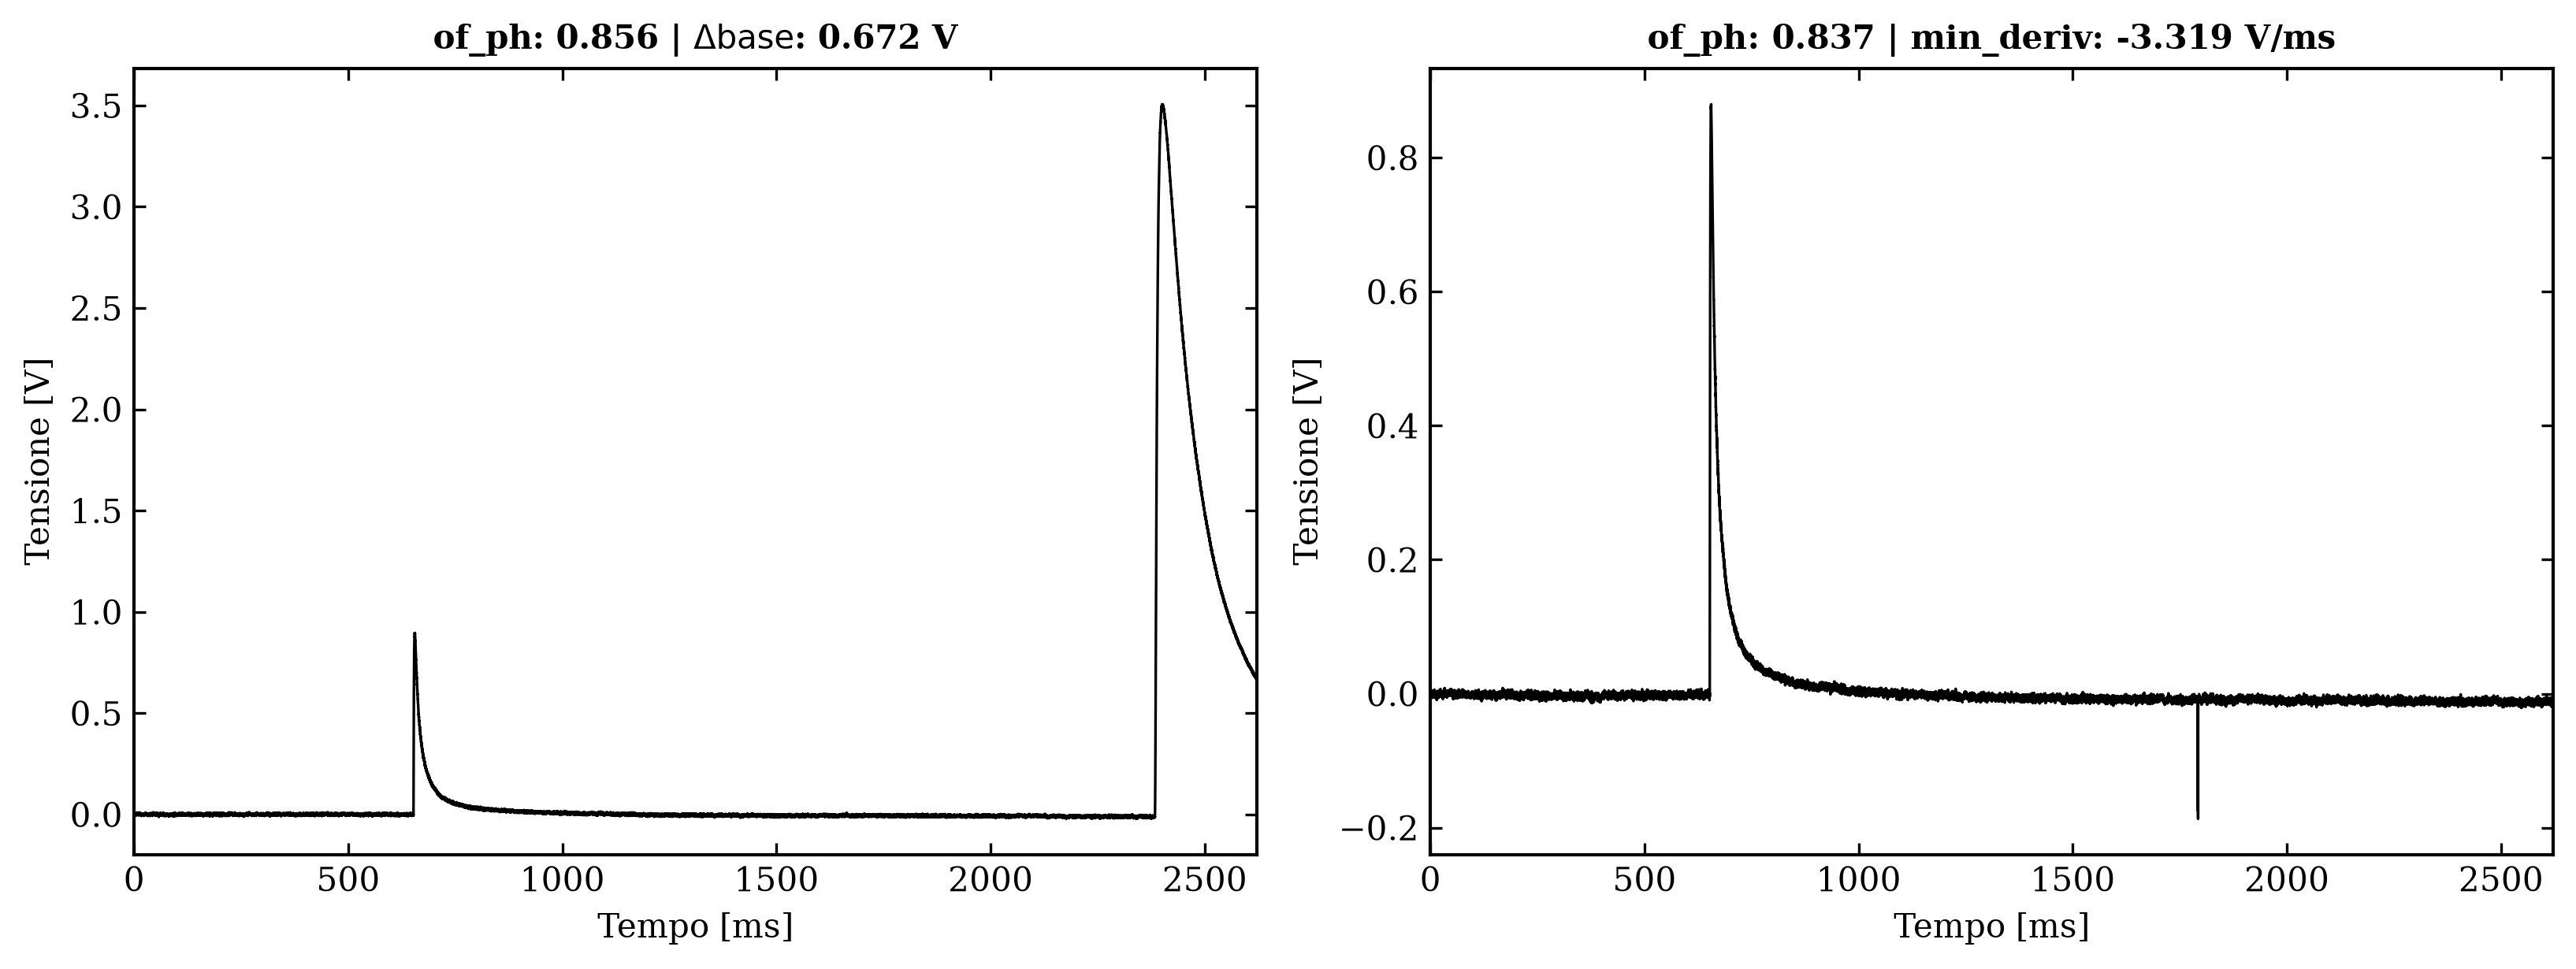
\includegraphics[width=0.9\textwidth]{figures/eventi_rigettati.png}
    \caption{Esempi di eventi fisici scartati dai tagli preliminari a causa di anomalie di baseline e problemi alla linearità del rivelatore: in particolare si nota il primo evento soggetto ad una elevata baseline difference dovuta ad un secondo evento verificatosi nella stessa finestra, mentre nel secondo caso una spike negativa dovuta probabilmente ad un'anomalai dell'elettronica.}
    \label{fig:eventi_rigettati}
\end{figure}

Tuttavia, questi tagli standard non sono in grado di intercettare i casi di \textit{pile-up}, in cui una seconda interazione avviene nella stessa finestra temporale senza alterare drasticamente la baseline finale. La presenza di un secondo picco altererebbe la forma media del template, compromettendo il calcolo dell'OF.

Per riconoscere ed eliminare questi eventi si impiega il \textbf{filtro di Savitzky-Golay}, un algoritmo che interpola localmente i punti con un polinomio di terzo grado, restituendo una traccia liscia. In particolare il polinomio è stato preso fittando 501 samples, 250 prima e 250 dopo il punto considerato. In seguito è stato preso il coefficiente costante del polinomio. Tale operazione è stata iterata per tutti i punti della finestra, ottenendo una forma d'onda in cui è stato abbattuto il rumore ad alta frequenza ma preservata la cuspide dell'impulso.
Sulla curva smussata viene applicato un algoritmo di ricerca dei massimi con due condizioni:
\begin{itemize}
    \item \textbf{Separazione temporale:} distanza minima tra picchi di $60\,\text{ms}$;
    \item \textbf{Prominenza minima:} ampiezza netta del picco di almeno $0.05\,\text{V}$.
\end{itemize}
Tale algoritmo non potrebbe essere applicato alla traccia grezza poiché intercetterebbe tutti i picchi dovuti alle fluttuazioni stocastiche del rumore.
Le tracce che manifestano più di un massimo valido vengono classificate come pile-up e scartate (Figura~\ref{fig:evento_rigettato_pileup}).

\begin{figure}[htbp]
    \centering
    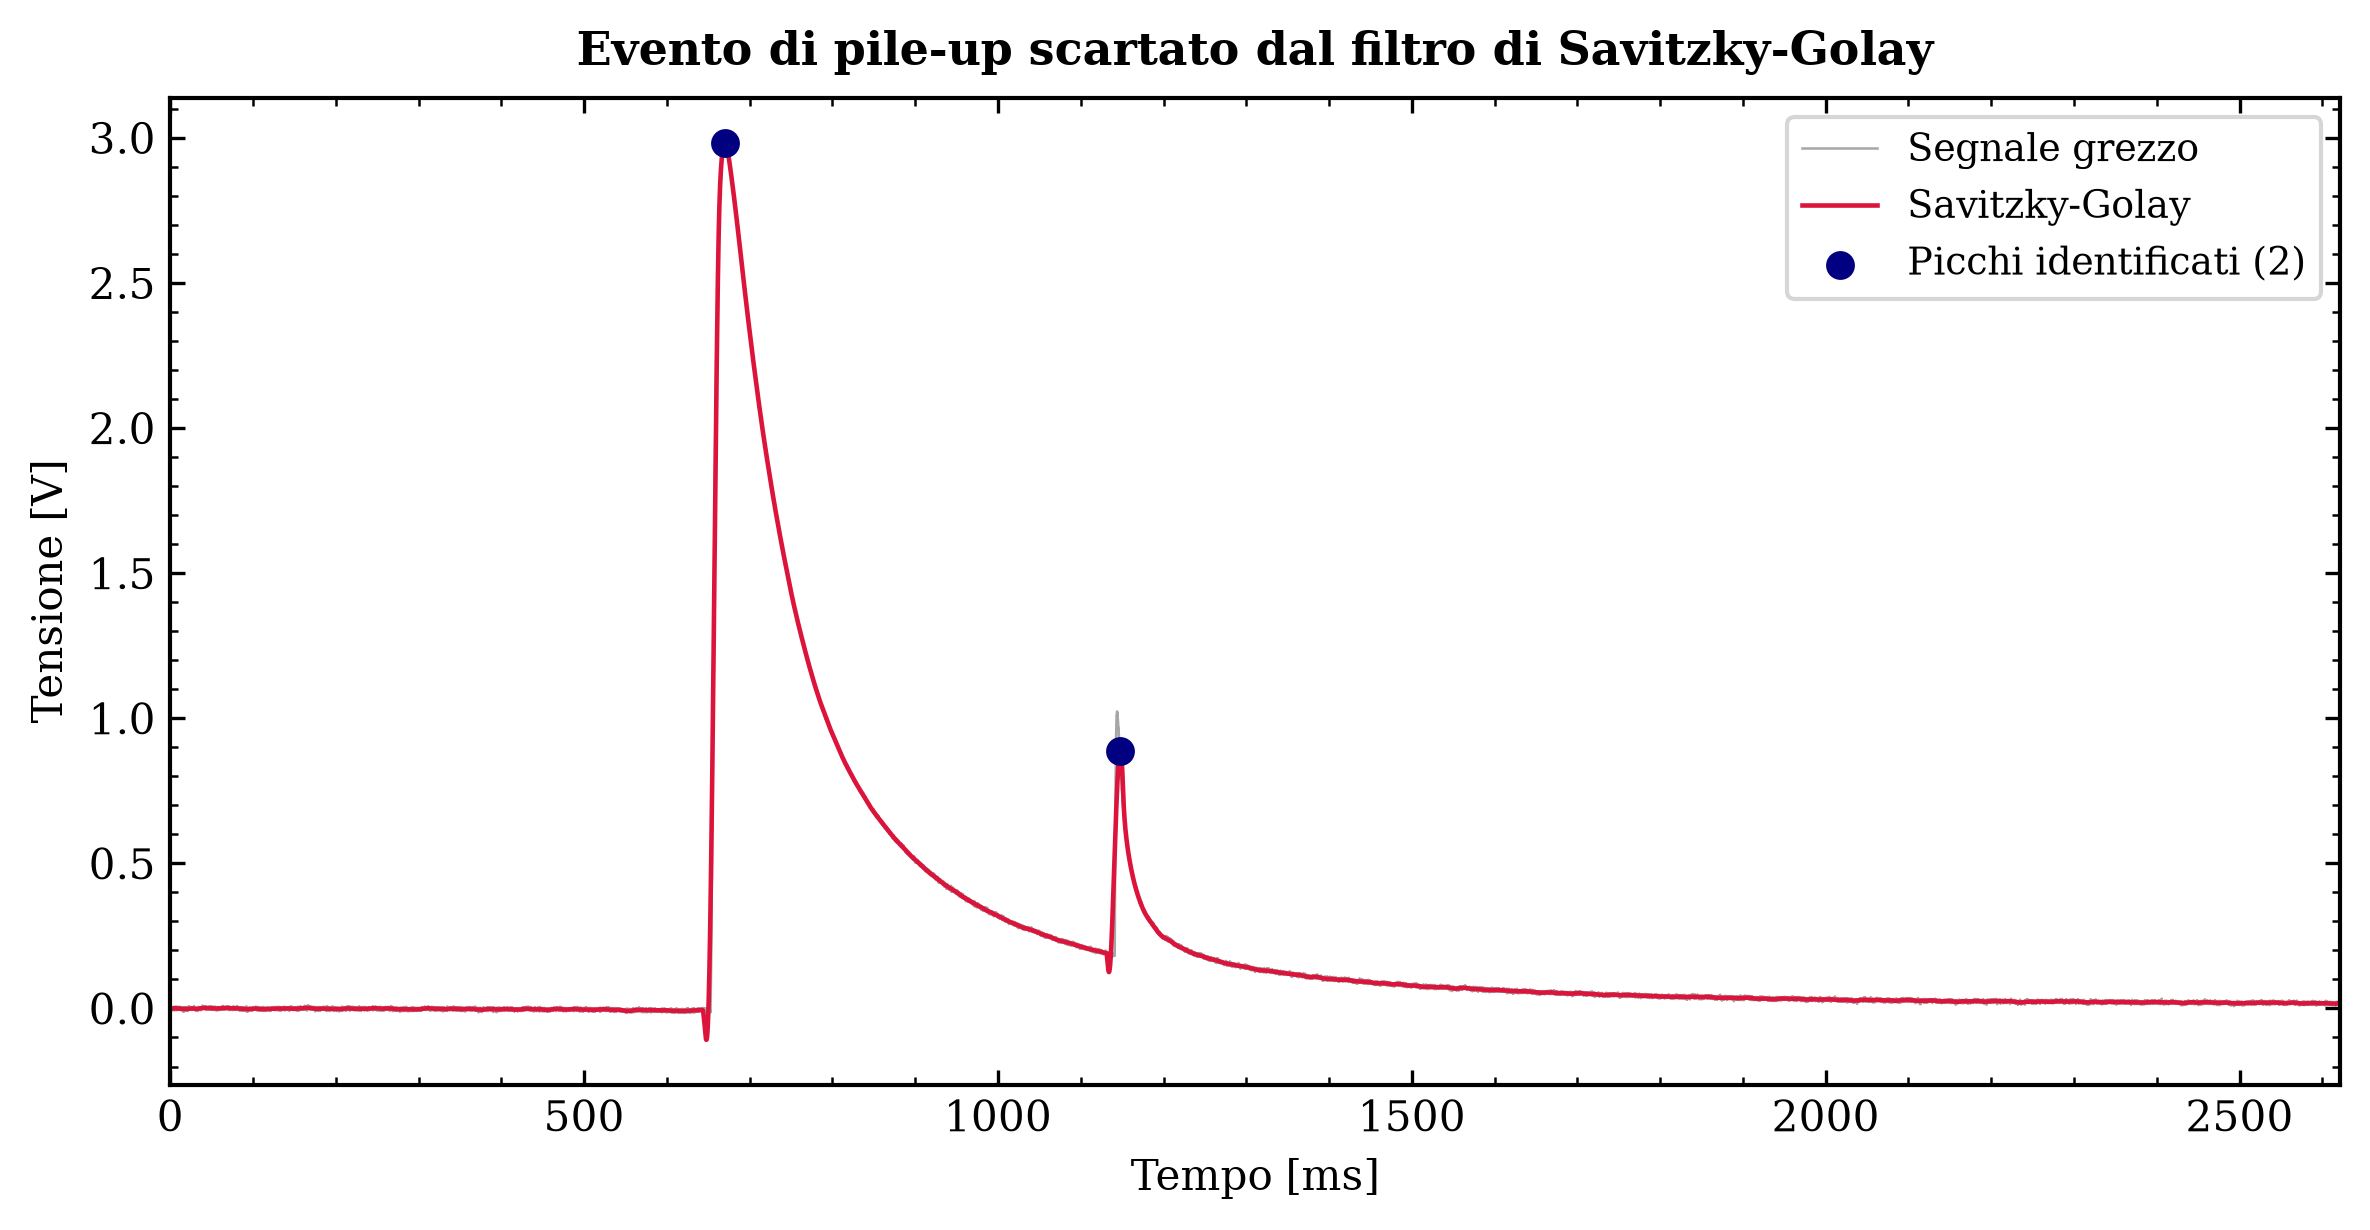
\includegraphics[width=0.88\textwidth]{figures/Esempio_Savitzky_Golay.png}
    \caption{Identificazione del pile-up tramite Savitzky-Golay: la curva smussata (in rosso) permette all'algoritmo di intercettare il secondo massimo locale ed escludere la traccia dal calcolo del template.}
    \label{fig:evento_rigettato_pileup}
\end{figure}

Mediando $337$ eventi di $^{55}\text{Fe}$ sopravvissuti ai tagli e normalizzando l'ampiezza al valore massimo unitario si ottiene il template fononico $s(t)$ (Figura~\ref{fig:confronto_templates}) e il corrispondente spettro di Fourier $S(f)$ (Figura~\ref{fig:FT_impulso_scremato}).

\begin{figure}[htbp]
        \centering
        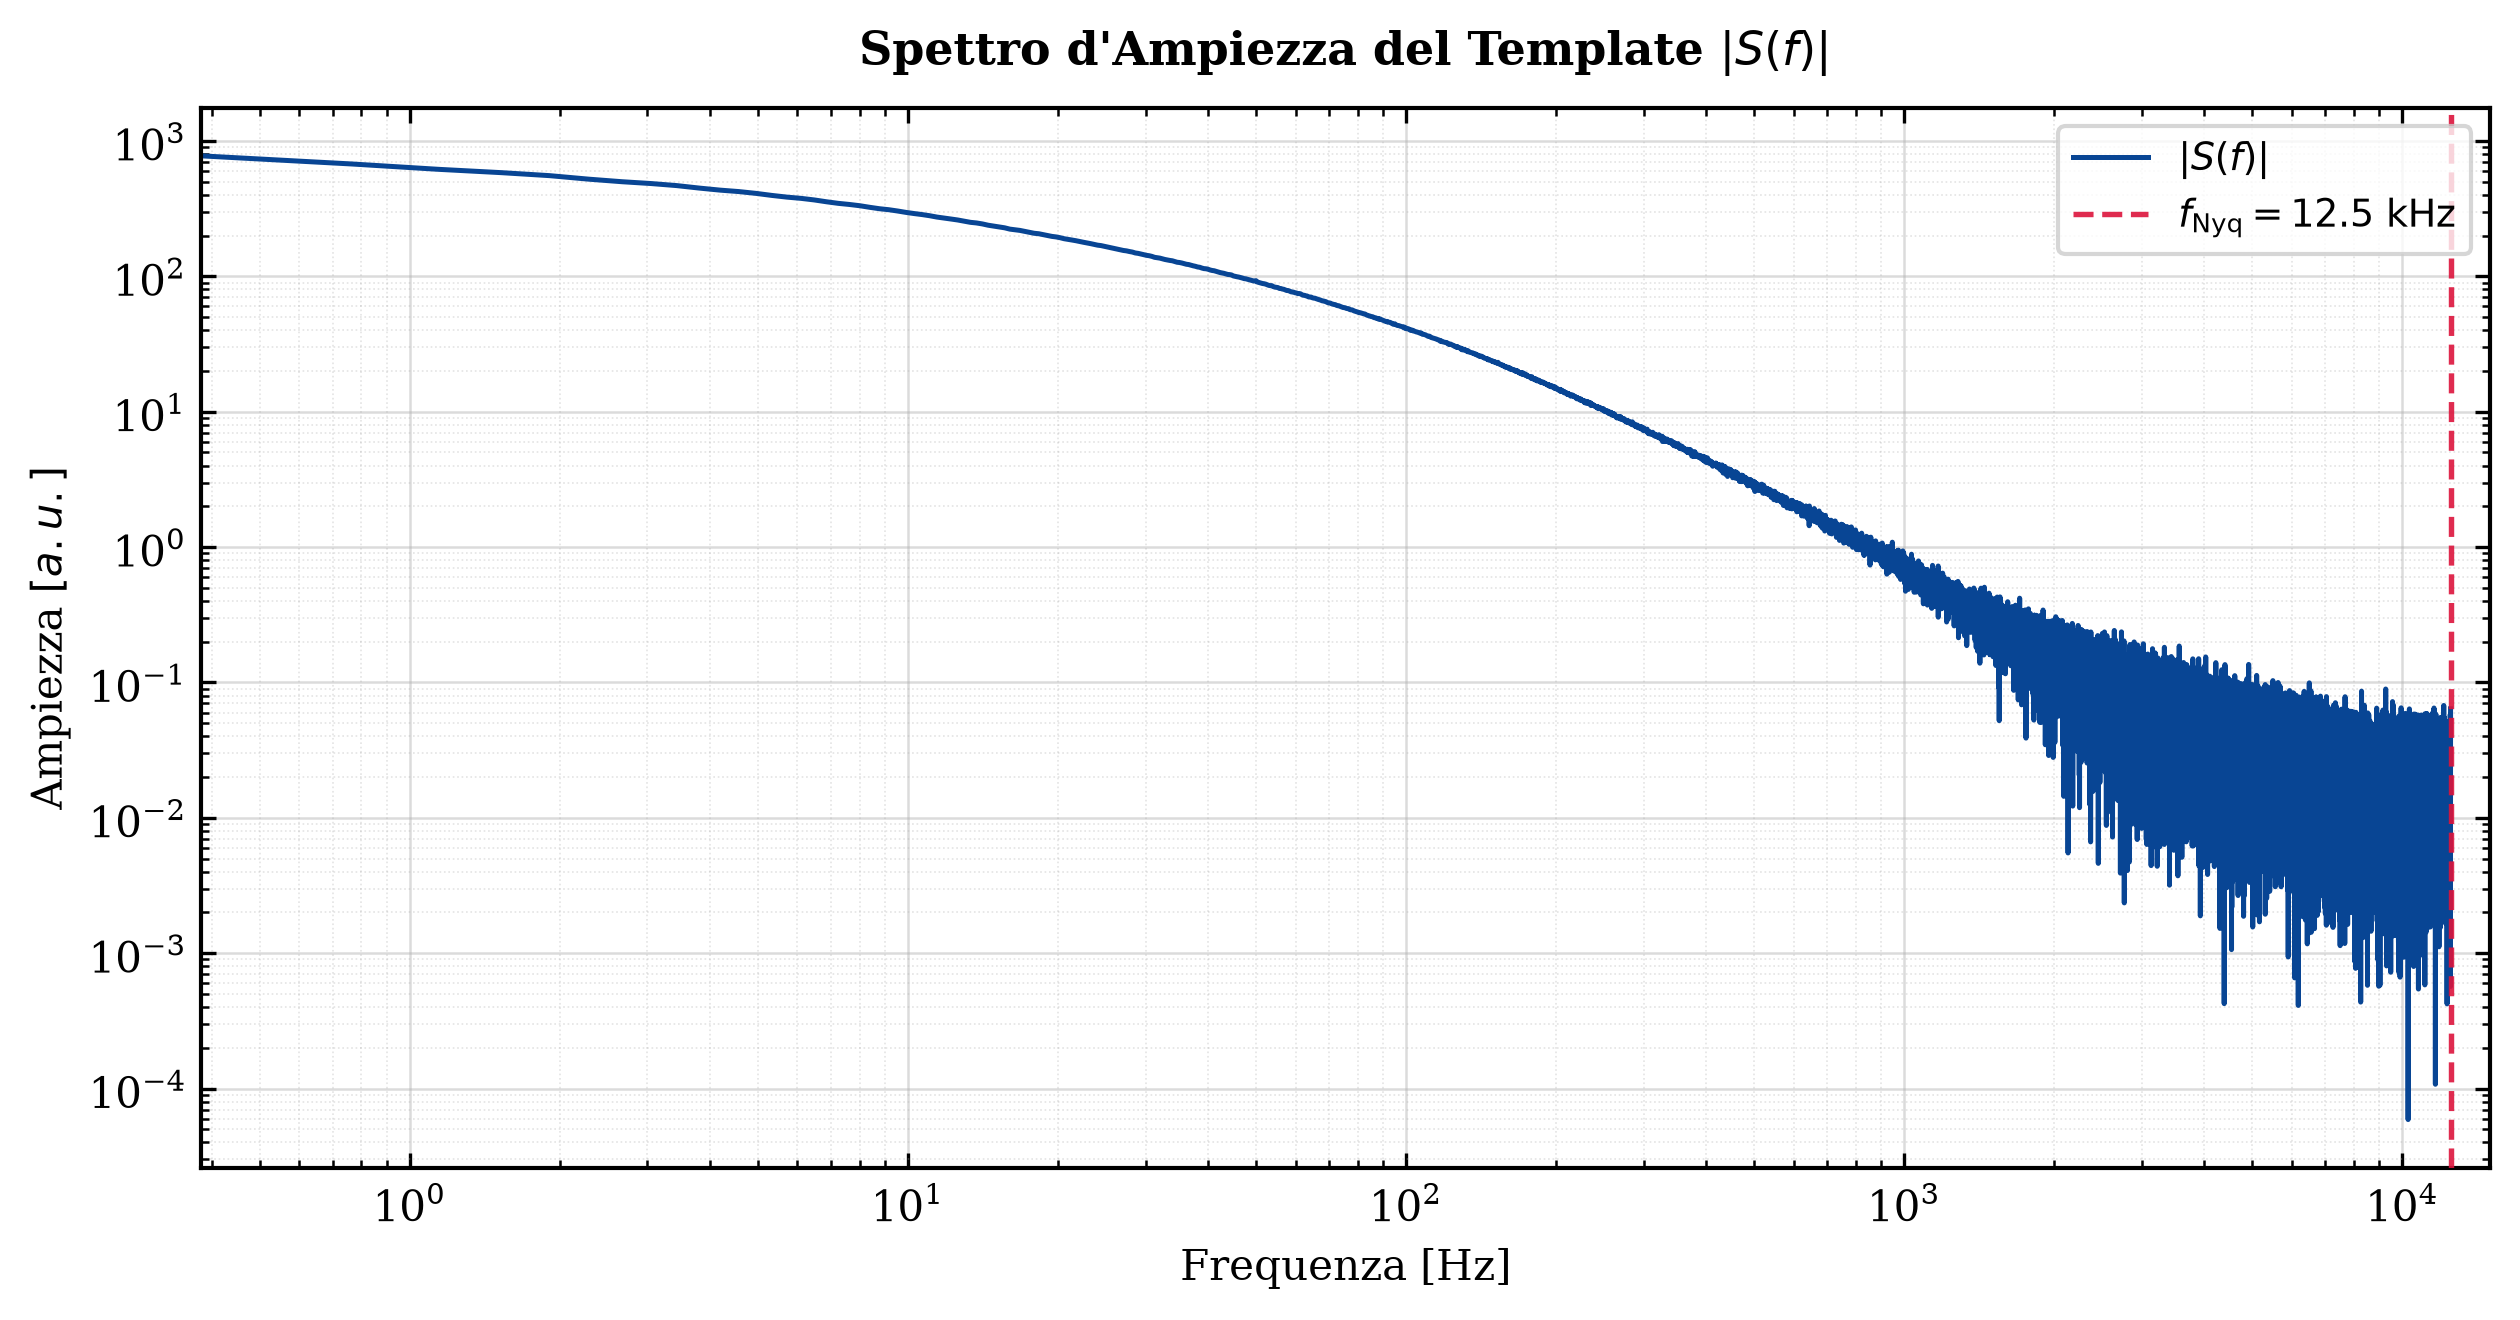
\includegraphics[width=0.85\linewidth]{figures/FT_impulso_scremato.png}
        \caption{Spettro di Fourier $S(f)$ del template fononico.}
        \label{fig:FT_impulso_scremato}
\end{figure}

% ------------------------------------------------------------------------------
\subsection{Template dei TestPulses e Confronto Morfologico}
\label{subsec:template_testpulse}

La risposta termica del rivelatore a un impulso di calore iniettato nell'heater non è del tutto identica a quella generata da una particella che colpisce il volume del cristallo. Sebbene entrambi i processi producano fononi termici, l'iniezione tramite heater avviene localmente sulla superficie e presenta una cinetica di diffusione leggermente differente.

Come illustrato nel confronto di Figura~\ref{fig:confronto_templates}, il TestPulse mostra un fronte di salita più dolce e un tempo di decadimento leggermente diverso rispetto all'impulso da particella. Per calibrare accuratamente i TestPulses senza introdurre disallineamenti di forma, è indispensabile costruire un template dedicato anche per essi.

\begin{figure}[htbp]
    \centering
    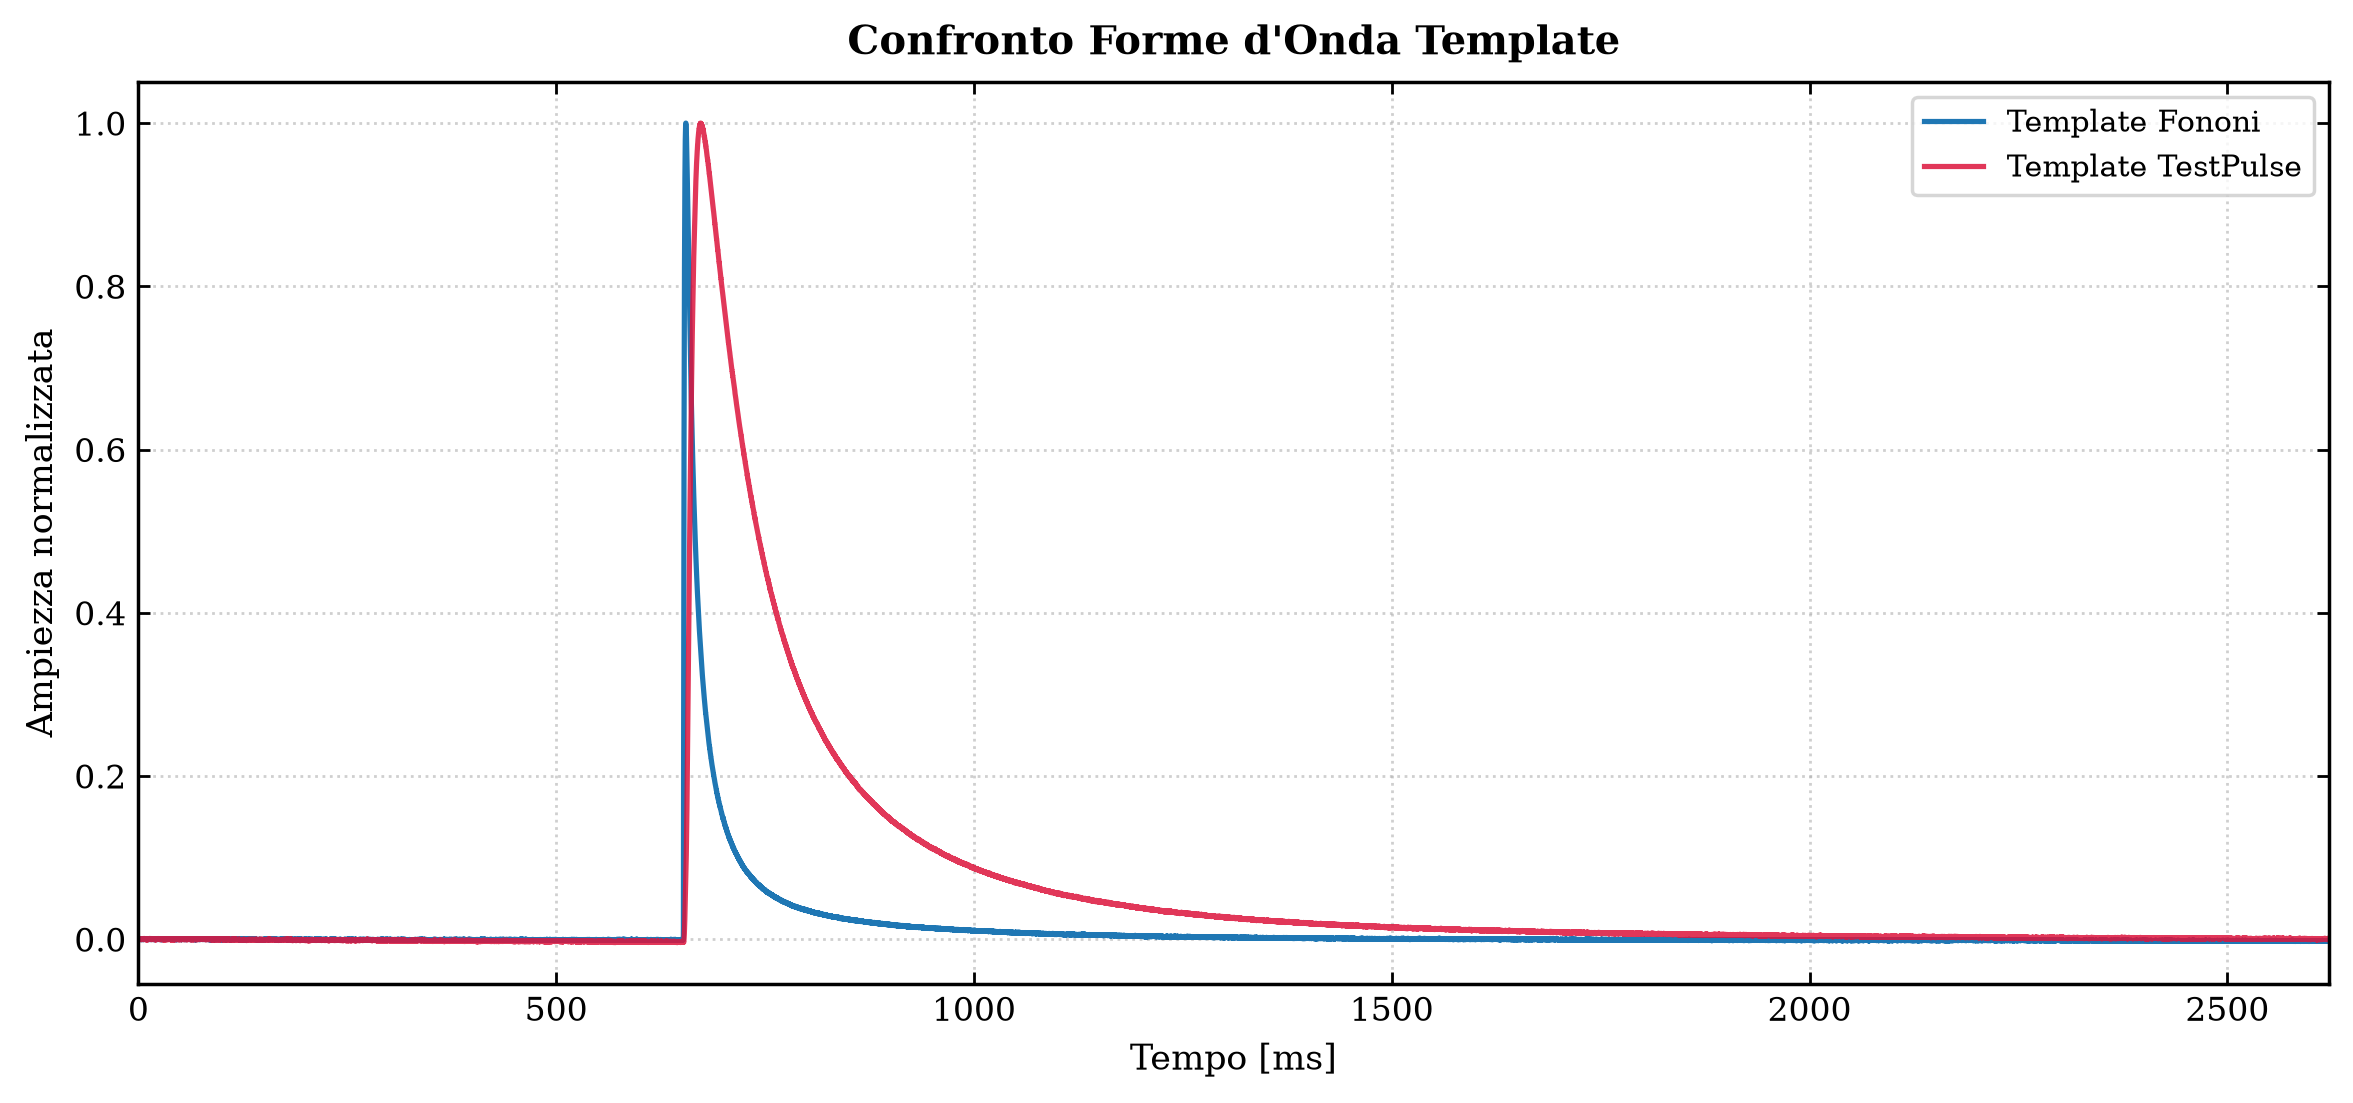
\includegraphics[width=0.85\textwidth]{figures/confronto_templates.png}
    \caption{Confronto normalizzato tra il template di particella ($^{55}\text{Fe}$) e il template ricavato dai TestPulses: l'impulso da particella presenta un tempo di salita più rapido.}
    \label{fig:confronto_templates}
\end{figure}

La procedura adottata per i TestPulses ricalca quella appena descritta: si selezionano impulsi non saturi generati a tensione costante ($V_{\text{inj}} = 1\,\text{V}$), si applicano i filtri su stabilità di baseline, assenza di pile-up e planarità della coda finale, e si media l'insieme delle tracce accettate normalizzando il picco a $1$.

% ==============================================================================
\section{Implementazione dell'Optimum Filter e Risultati}
\label{sec:applicazione_OF}
% ==============================================================================

Disponendo dell'NPS e del template di forma, la funzione di trasferimento $H(f)$ (Figura~\ref{fig:OF_complete}) viene utilizzata per estrarre l'esatta ampiezza di un evento secondo i seguenti passaggi:
\begin{enumerate}
    \item Si calcola la FT del segnale e la si moltiplica frequenza per frequenza per $H(f)$;
    \item Si esegue l'antitrasformata inversa (IFT) per tornare nel dominio del tempo;
    \item L'ampiezza dell'evento viene estratta dal picco del segnale filtrato, che risulta privo delle componenti oscillanti ad alta frequenza e delle interferenze a $50\,\text{Hz}$.
    \item L'evento viene ricostruito moltiplicando punto per punto il template per l'ampiezza ricostruita dal filtro.
\end{enumerate}

\begin{figure}[htbp]
    \centering
    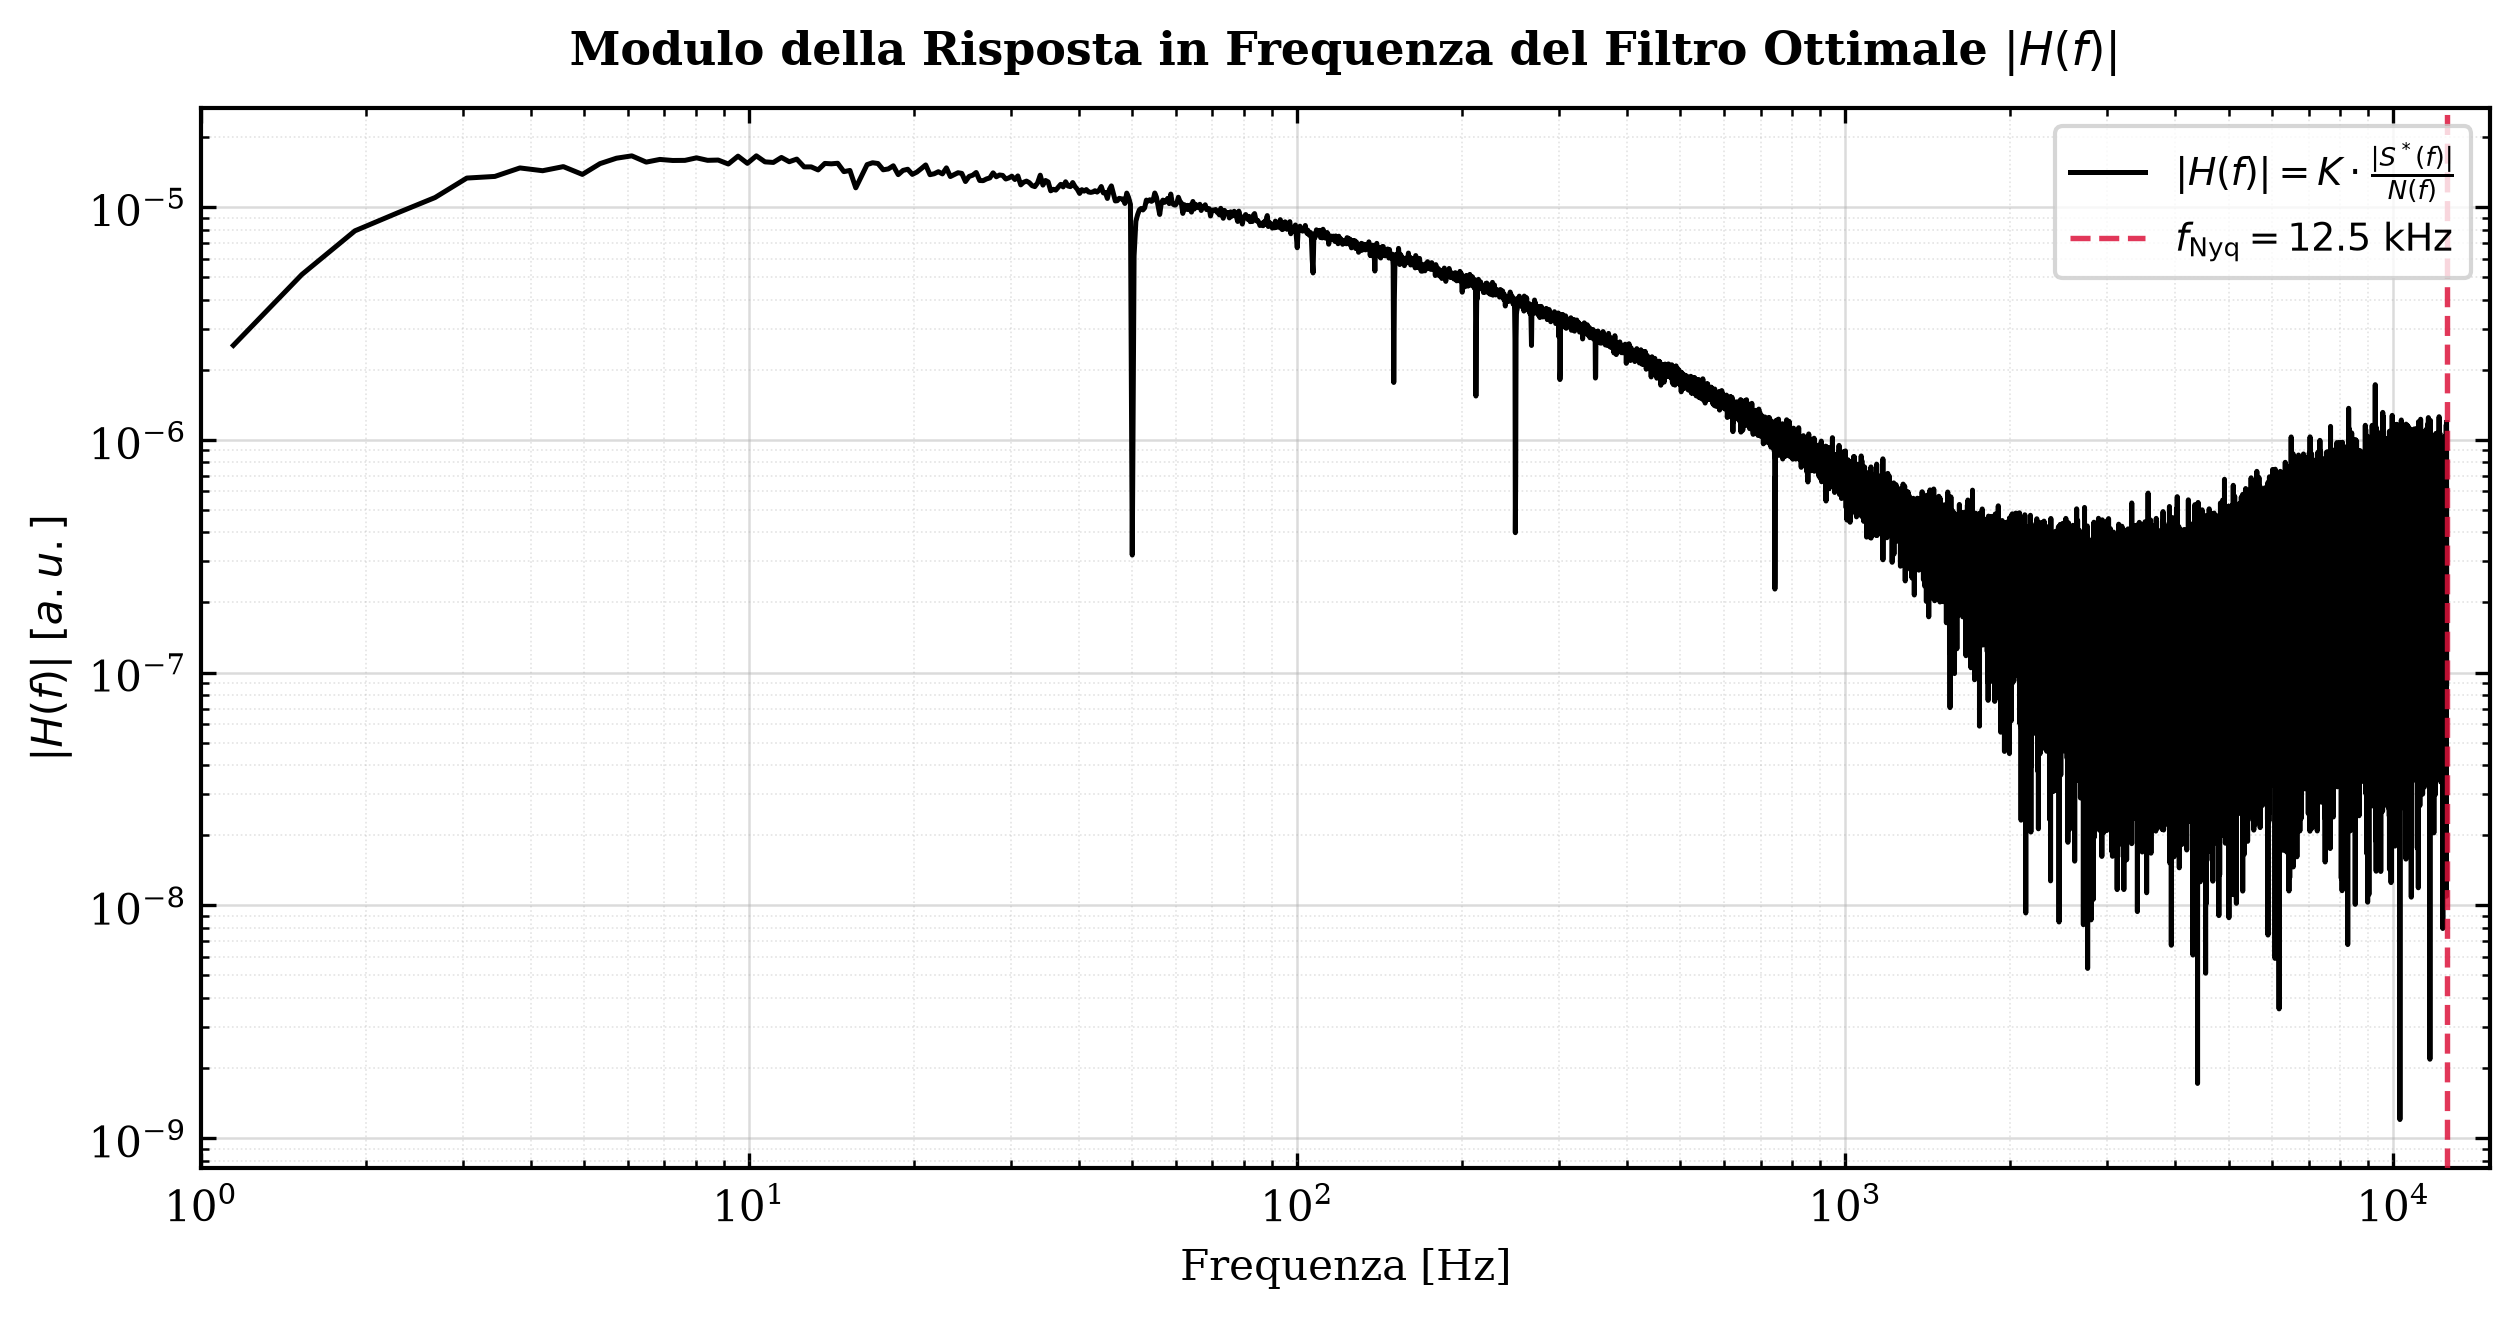
\includegraphics[width=0.8\textwidth]{figures/OF_rms.png}
    \caption{Modulo della funzione di trasferimento $H(f)$ dell'Optimum Filter per un evento di particella: si nota l'accentuata soppressione in corrispondenza del rumore di rete ($50\,\text{Hz}$) e alle alte frequenze.}
    \label{fig:OF_complete}
\end{figure}

Un esempio di applicazione su un impulso di piccola ampiezza ($V_{\text{inj}} = 0.5\,\text{V}$) è mostrato in Figura~\ref{fig:ricostruzione_TP}. La traccia grezza, inizialmente dominata dalle fluttuazioni casuali, viene pulita efficacemente dall'OF, consentendo una misura precisa e non distorta dell'altezza dell'impulso.

\begin{figure}[htbp]
    \centering
    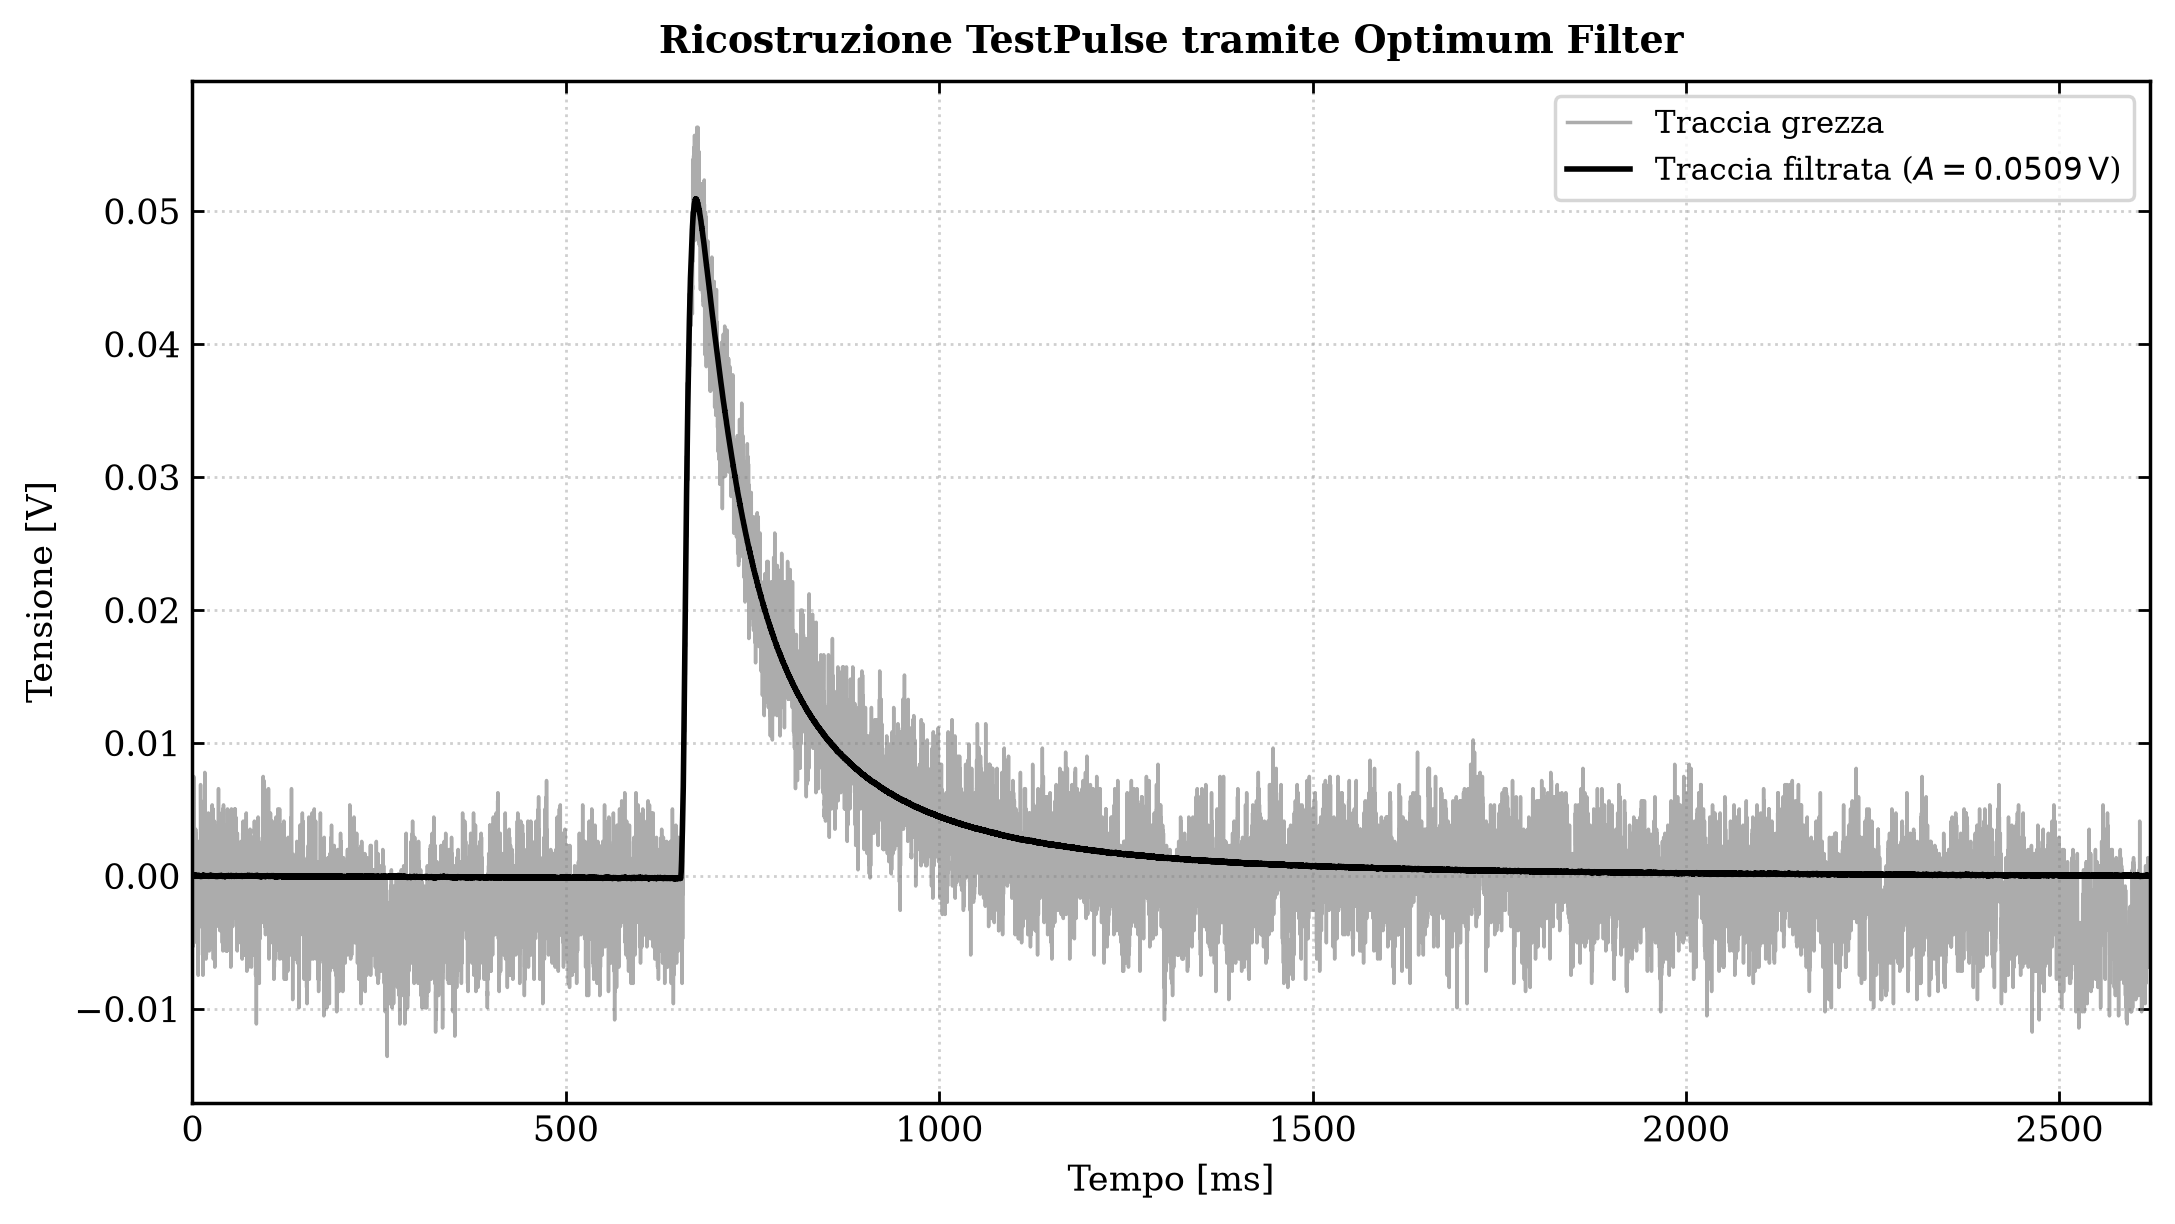
\includegraphics[width=0.7\textwidth]{figures/esempio_ric_TP.png}
    \caption{Applicazione dell'Optimum Filter a un TestPulse a bassa energia: confronto tra traccia grezza (grigio) e ricostruzione ottenuta scalando il template sull'ampiezza stimata (nero).}
    \label{fig:ricostruzione_TP}
\end{figure}

% ==============================================================================
\section{Rumore Residuo e Determinazione della Soglia di Trigger}
\label{sec:trigger_noise}
% ==============================================================================

to be continue... %3 
\clearpage{\thispagestyle{empty}\cleardoublepage}
\input{chapters/04_cap.tex} %4
\clearpage{\thispagestyle{empty}\cleardoublepage}

%------------------------------- CONCLUSIONI
\phantomsection
\addcontentsline{toc}{chapter}{Conclusioni}
\input{chapters/99_conclusioni}
\clearpage{\thispagestyle{empty}\cleardoublepage}

%------------------------------ BIBLIOGRAFIA 
\phantomsection
\printbibliography
\addcontentsline{toc}{chapter}{Bibliografia}
\clearpage{\thispagestyle{empty}\cleardoublepage}

%----------------------------- RINGRAZIAMENTI  
\phantomsection
\addcontentsline{toc}{chapter}{Ringraziamenti}
\input{chapters/Ringraziamenti}
\clearpage{\thispagestyle{empty}\cleardoublepage}

\end{document}